\chapter{Experimentación}
En esta sección se explican los experimentos realizados hasta alcanzar la versión final del clasificador siguiendo los pasos propuestos en la metodología. Delimitar las pruebas que se van a realizar en un proyecto es fundamental para concentrar los esfuerzos y cumplir con los objetivos en plazo. Al tratarse de un proyecto de investigación, realizo experimentos iniciales, evalúo los resultados y vuelvo a realizar experimentos hasta alcanzar unos resultados que cumplan con los objetivos.

La implementación de los experimentos realizados se encuentra en el repositorio de GitHub del proyecto \cite{repository}. La raíz del repositorio contiene los siguientes elementos:

\dirtree{%
    .1 /.
    .2 datasets/.
    .2 experiments/\DTcomment{implementación del TFG}.
    .2 papers/\DTcomment{algunas de las publicaciones utilizadas en su desarrollo}.
    .2 report/\DTcomment{memoria en formato \LaTeX}.
    .2 slides/.
    .2 README.md.
}

\newpage
\section{Transformaciones sobre el \textit{dataset}}
Tras recibir el \textit{dataset} y normalizar el tamaño de las imágenes, procedo a aplicar las tres secuencias de \textit{data augmentation} que he explicado en el capítulo anterior.

El \textit{dataset} original y los derivados obtenidos al aplicar \textit{data augmentation} se almacenarán en el directorio \textit{datasets/} del repositorio, como se describe en el siguiente árbol:

\vspace{0.2cm}
\dirtree{%
    .1 datasets/.
    .2 negev/.
    .3 articles\_molecules/\DTcomment{ejemplos positivos}.
    .4 preprocess256/\DTcomment{imágenes 256x256}.
    .5 aug/\DTcomment{\textit{data augmentation} 1}. 
    .6 1.png.
    .6 2.png.
    .6 \ldots.
    .5 aug2/\DTcomment{\textit{data augmentation} 2}.
    .6 1.png.
    .6 2.png.
    .6 \ldots.
    .5 aug3/\DTcomment{\textit{data augmentation} 3}.
    .6 1.png.
    .6 2.png.
    .6 \ldots.
    .5 1.png.
    .5 2.png.
    .5 \ldots.
    .4 1.png.
    .4 2.png.
    .4 \ldots.
    .3 not\_molecules/\DTcomment{ejemplos negativos}.
}

El código que me permitirá realizar estas transformaciones se encuentra en los siguientes archivos:

\vspace{0.2cm}
\dirtree{%
    .1 experiments/.
    .2 taming\_transformers/.
    .3 data\_generation\_and\_augmentation.ipynb.
    .3 functions.py.
}

\noindent \textit{{data\_generation\_and\_augmentation.ipynb}} contiene el código que pre-procesa las imágenes, transformándolas de forma que tengan el mismo tamaño, y que aplica las tres secuencias de \textit{data augmentation} que he comentado.

\noindent \textit{functions.py} declara funciones utilizadas por todos este cuaderno.

\noindent Aunque no se mencionan aquí, existen otros directorios y ficheros auxiliares que permiten funcionar a estos.

Comienzo por \textit{data augmentation} 1. Al aplicarla se obtienen los resultados mostrados en la Figura \ref{fig:data-aug1}.

\begin{figure}[H]
\centering
    \begin{subfigure}{.25\textwidth}
        \centering
        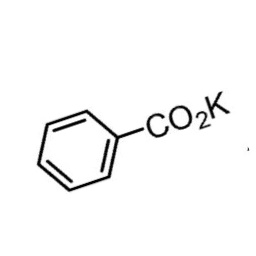
\includegraphics[width=1\linewidth]{imagenes/aug/180.jpg}
    \end{subfigure}%
    \begin{subfigure}{.25\textwidth}
        \centering
        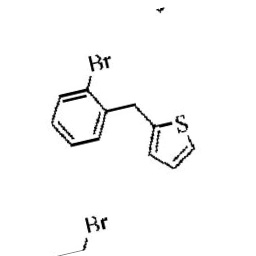
\includegraphics[width=1\linewidth]{imagenes/aug/193.jpg}
    \end{subfigure}%

    \bigskip

    \begin{subfigure}{.25\textwidth}
        \centering
        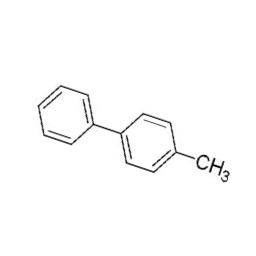
\includegraphics[width=1\linewidth]{imagenes/aug/224.jpg}
    \end{subfigure}%
    \begin{subfigure}{.25\textwidth}
        \centering
        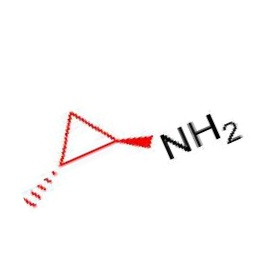
\includegraphics[width=1\linewidth]{imagenes/aug/370.jpg}
    \end{subfigure}

    \caption{Imágenes generadas aplicando \textit{data augmentation} 1}
    \label{fig:data-aug1}
\end{figure}

Se aprecian leves rotaciones y estiramientos de las imágenes, sin existir gran diferencia con las originales. Al estar aplicando tres veces la transformación sobre el conjunto de datos, puede que los cambios sean demasiado suaves dando lugar a imágenes muy similares. A continuación, observemos los resultados de \textit{data augmentation} 2 en la Figura \ref{fig:data-aug2}.

\begin{figure}[H]
\centering
    \begin{subfigure}{.23\textwidth}
        \centering
        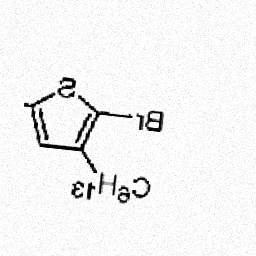
\includegraphics[width=1\linewidth]{imagenes/aug2/169.jpg}
    \end{subfigure}%
    \begin{subfigure}{.23\textwidth}
        \centering
        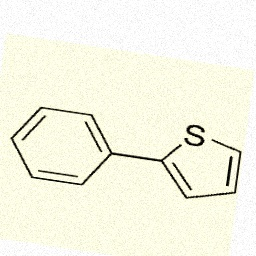
\includegraphics[width=1\linewidth]{imagenes/aug2/188.jpg}
    \end{subfigure}%

    \bigskip

    \begin{subfigure}{.23\textwidth}
        \centering
        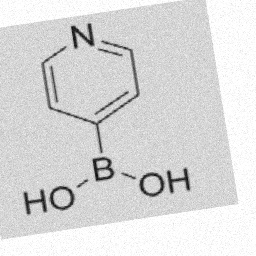
\includegraphics[width=1\linewidth]{imagenes/aug2/221.jpg}
    \end{subfigure}%
    \begin{subfigure}{.23\textwidth}
        \centering
        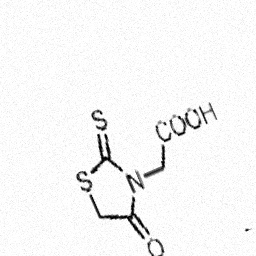
\includegraphics[width=1\linewidth]{imagenes/aug2/222.jpg}
    \end{subfigure}

    \caption{Imágenes generadas aplicando \textit{data augmentation} 2}
    \label{fig:data-aug2}
\end{figure}

En este caso se observan más cambios fundamentalmente debidos a las variaciones en contraste, al uso de ruido gaussiano y a la multiplicación, responsable de los cambios de color, ya que a veces se aplica a canales independientes. Puede ser una transformación adecuada, ya que añade diversidad al conjunto sin cambios demasiado pronunciados. 

Por último, comprobemos los resultados que se obtienen al aplicar \textit{data augmentation} 3 en la Figura \ref{fig:data-aug3}.

\begin{figure}[H]
\centering
    \begin{subfigure}{.23\textwidth}
        \centering
        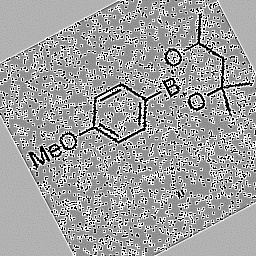
\includegraphics[width=1\linewidth]{imagenes/aug3/175.jpg}
    \end{subfigure}%
    \begin{subfigure}{.23\textwidth}
        \centering
        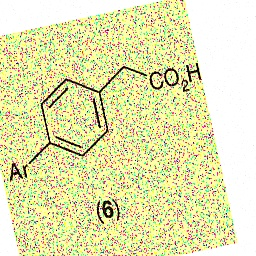
\includegraphics[width=1\linewidth]{imagenes/aug3/183.jpg}
    \end{subfigure}%

    \bigskip

    \begin{subfigure}{.23\textwidth}
        \centering
        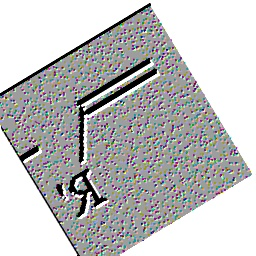
\includegraphics[width=1\linewidth]{imagenes/aug3/225.jpg}
    \end{subfigure}%
    \begin{subfigure}{.23\textwidth}
        \centering
        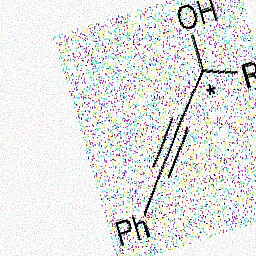
\includegraphics[width=1\linewidth]{imagenes/aug3/347.jpg}
    \end{subfigure}

    \caption{Imágenes generadas aplicando \textit{data augmentation} 3}
    \label{fig:data-aug3}
\end{figure}

En esta última versión las transformaciones son bastante agresivas. Se introduce mucho ruido en las imágenes y las rotaciones y los cambios en el contraste son fuertes.

Para entrenar el clasificador, seguramente las imágenes más adecuadas sean las generadas por \textit{data augmentation} 2. Son las más equilibradas, ya que la versión 1 apenas introduce cambios y la versión 3 añade demasiado ruido, creando imágenes que no se corresponden con la realidad y por tanto pueden penalizar el rendimiento del modelo.

\newpage
\section{Generación de imágenes sintéticas}

Sobre los cuatro conjuntos de datos se entrenarán modelos con diferente número de épocas, desde 70 hasta 170, aumentando de 20 en 20. De esta forma tendré $4 * |[70, 90, 110, 130, 150, 170]| = 4 * 6 = 24$ modelos diferentes.

Una vez entrenados, probaré a generar imágenes a partir de estos para ver cuál se comporta mejor. Para ello, debo introducirles algún tipo de imagen de entrada.

La generación de imágenes se va a realizar utilizando el modelo desarrollado por Esser et al. \cite{esser2021taming}, descrito en la Sección \label{st:taming-transformers}. El código en el que se realizan los experimentos con el generador se encuentra en los siguientes archivos:

\vspace{0.2cm}
\dirtree{%
    .1 experiments/\DTcomment{implementación del TFG}.
    .2 taming\_transformers/\DTcomment{generador de imágenes}.
    .3 taming-transformers/\DTcomment{implementación del generador}.
    .3 sample\_and\_clean\_molecules.ipynb.
    .3 sampling\_experiment.ipynb.
    .3 functions.py.
}

\noindent El subdirectorio \textit{taming-transformers/} contiene la implementación del modelo generativo proporcionada por sus autores \cite{taming-transformers-github}. 

\noindent \textit{sampling\_experiment.ipynb} es un cuaderno que, una vez entrenados los modelos, permite cargarlos y generar imágenes sintéticas a partir de otra imagen de entrada. Se utiliza para comprobar a partir de que \textit{dataset} se generan mejores resultados y con qué número de épocas. Es importante saber que este modelo generativo necesita de una imagen condicionante para generar una imagen sintética: se realizarán pruebas con distintos tipos, entre ellas ruido, para comprobar con cuáles se obtienen mejores resultados.

\noindent \textit{sample\_and\_clean\_molecules.ipynb}  permite generar un lote de imágenes sintéticas indicando el modelo que queremos utilizar y las propiedades del ruido, en concreto de ruido Perlín, ruido que explicaremos en los experimentos. También creará el \textit{dataset} final que contiene \textit{hard negatives}.

\noindent \textit{functions.py} declara funciones utilizadas por todos estos cuadernos.

\newpage
En las páginas siguientes se muestran los resultados. Cada fila corresponde a una imagen de entrada al modelo. En las columnas, la primera muestra la imagen de entrada mientras que cada una de las siguientes corresponde con un modelo entrenado durante x épocas, desde 70 hasta 170 (70, 90, 110, 130, 150, 170).

Se puede observar como la versión sin \textit{data augmentation} no funciona bien, produce imágenes sin apenas estructura. Esto se debe a que solo se utilizan 162 imágenes, cifra muy baja para una arquitectura de deep learning como es un \textit{transformer}. Con \textit{data augmentation} 1 tampoco se observan resultados de buena calidad, puede que algo mejores que en el caso anterior pero sin muchas diferencias.

Es en \textit{data augmentation} 2 cuando ya se empiezan a ver mayores diferencias. El uso de transformaciones más fuertes crea un conjunto heterogéneo de imágenes y el modelo puede aprender más características de estas. Los resultados son aceptables, aunque el cambio de color que las transformaciones producían en algunas imágenes de entrenamiento ha dado lugar a fondos grisáceos en sus homólogas sintéticas. 

Con el tercer \textit{data augmentation} estos fondos grisáceos son mucho más marcados. Recordar que estas transformaciones eran mucho más fuertes, por lo que se traslada a las imágenes sintéticas.


\begin{figure}[H]
\centering
    \caption{Resultados de entrenar los modelos sobre el conjunto de datos sin \textit{data augmentation}. La primera columna representa la imagen de entrada, el resto los diferentes modelos entrenados desde 70 hasta 170 épocas, tomadas de 20 en 20.} 
    \fbox{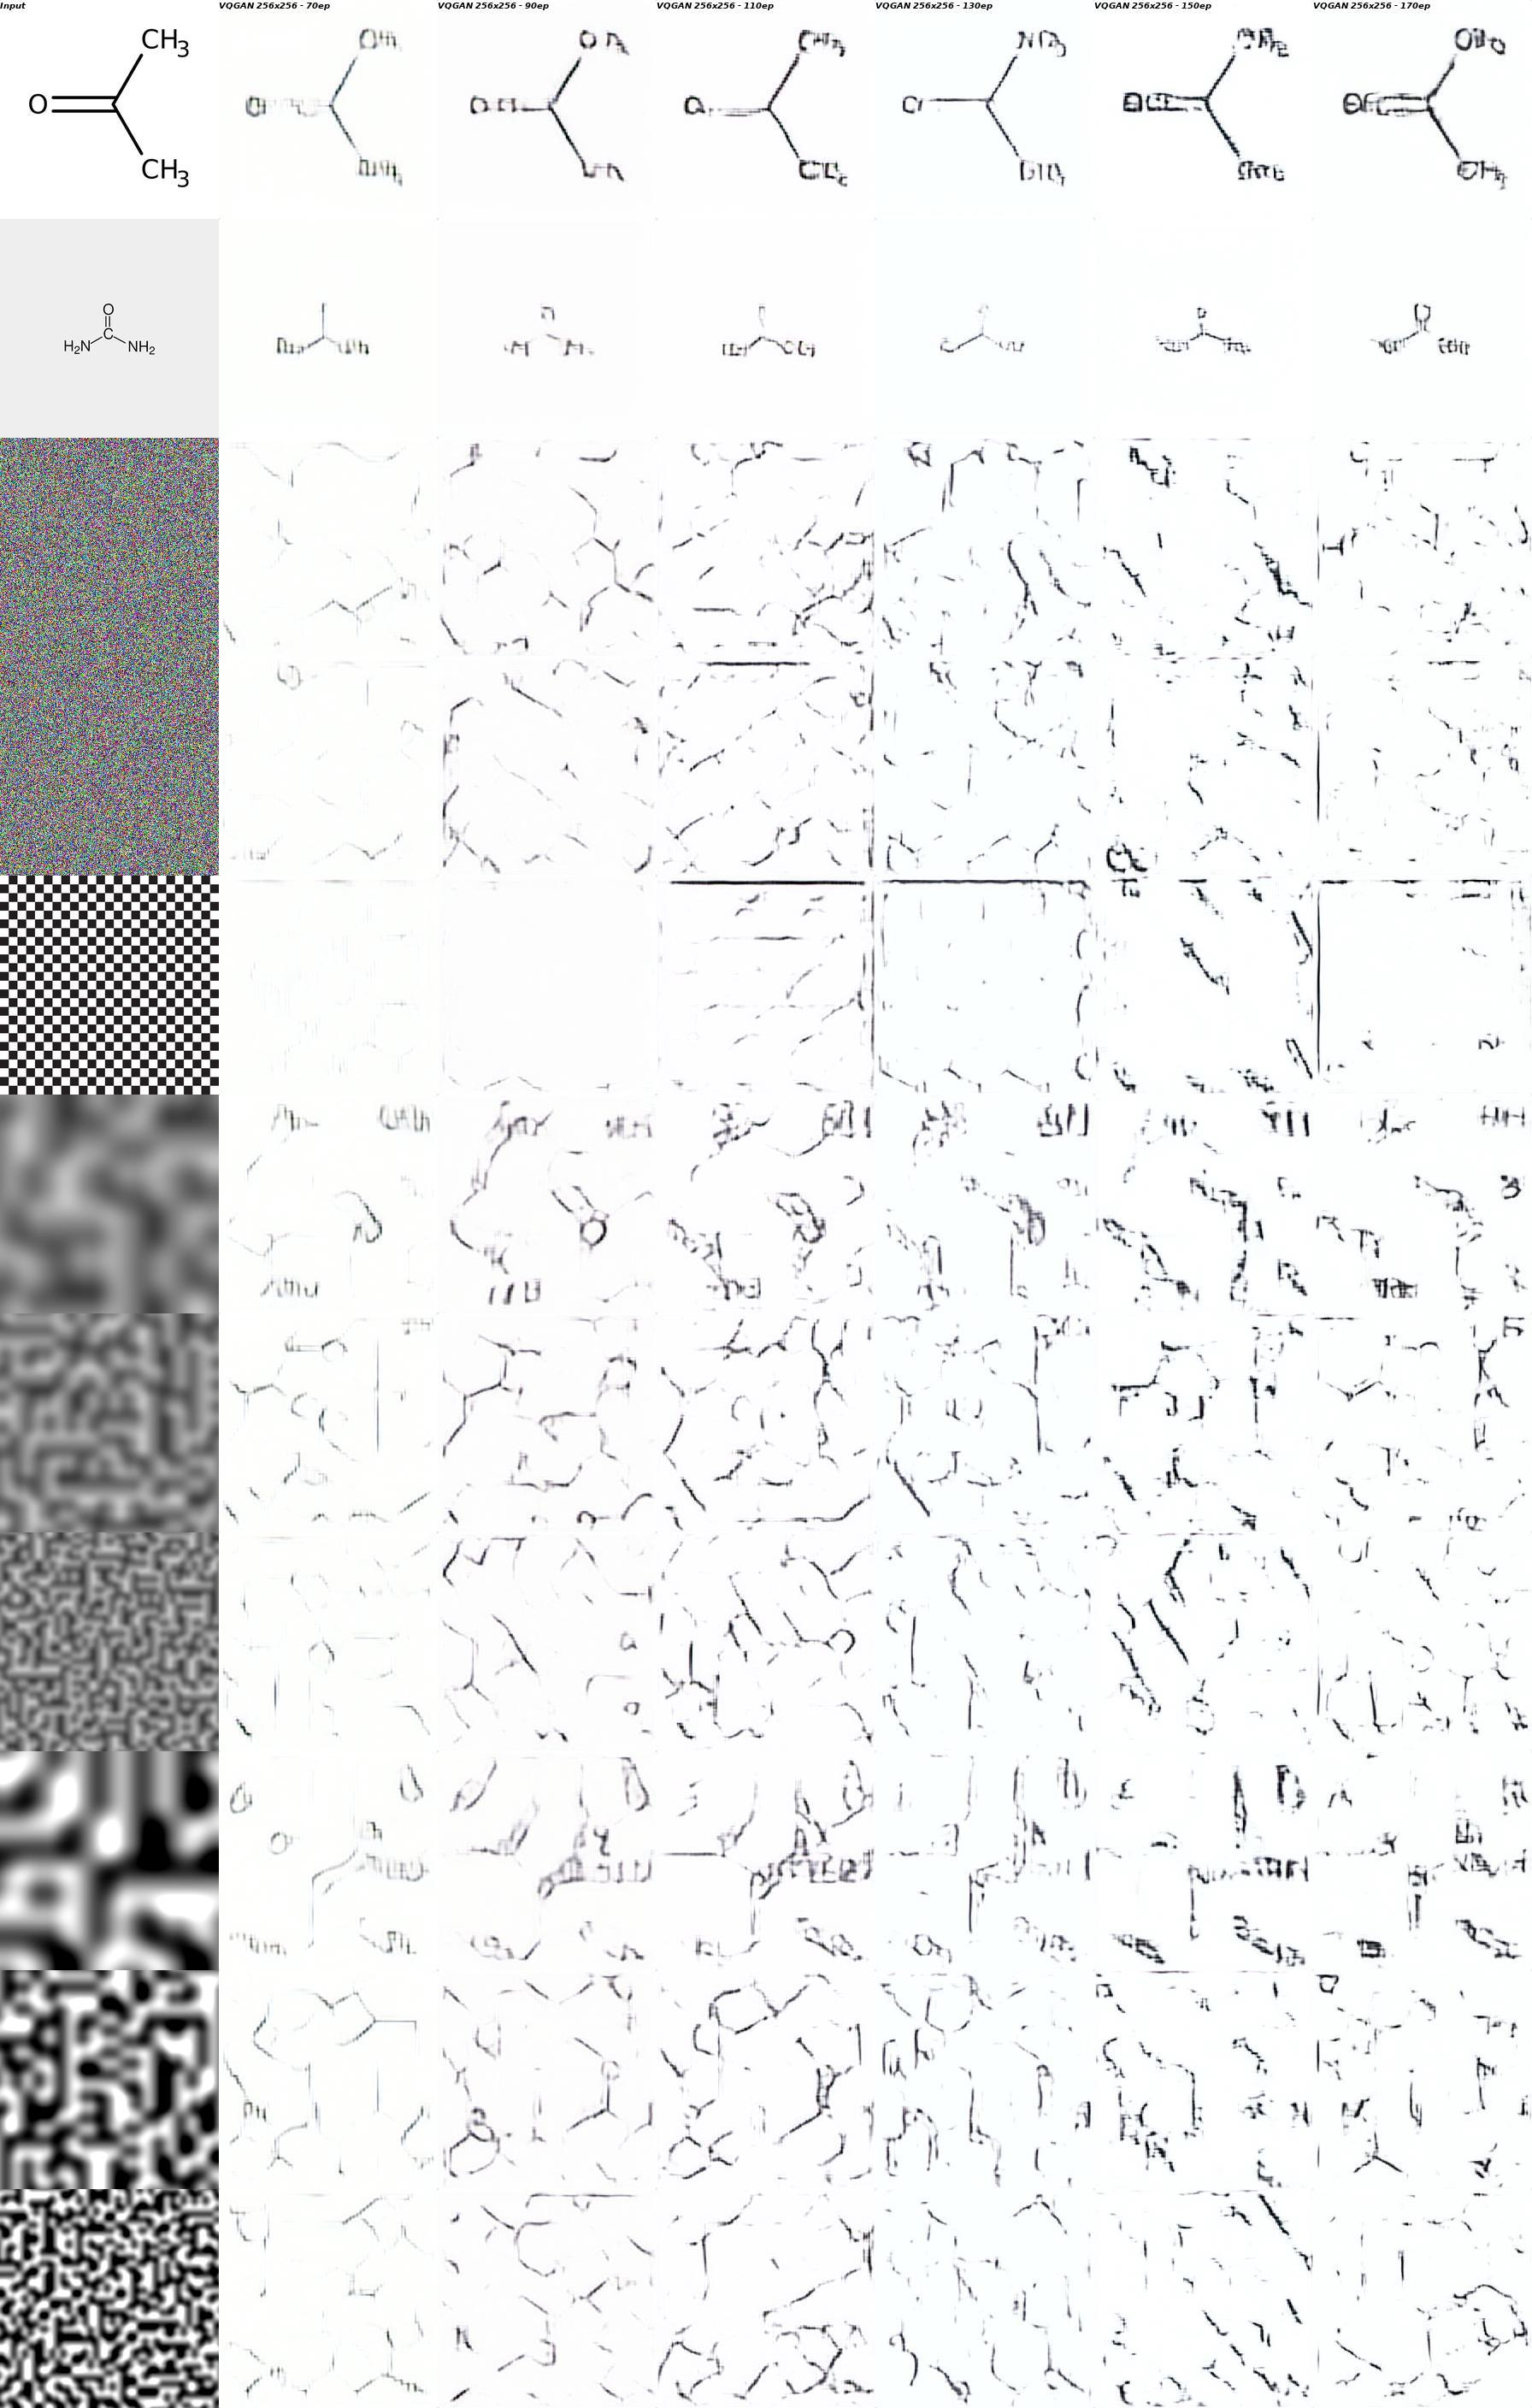
\includegraphics[scale=0.2]{imagenes/image_generation/256/256_1.jpg}}  
    \label{fig:synthetic_molecules}
\end{figure}

\begin{figure}[H]
\centering
    \fbox{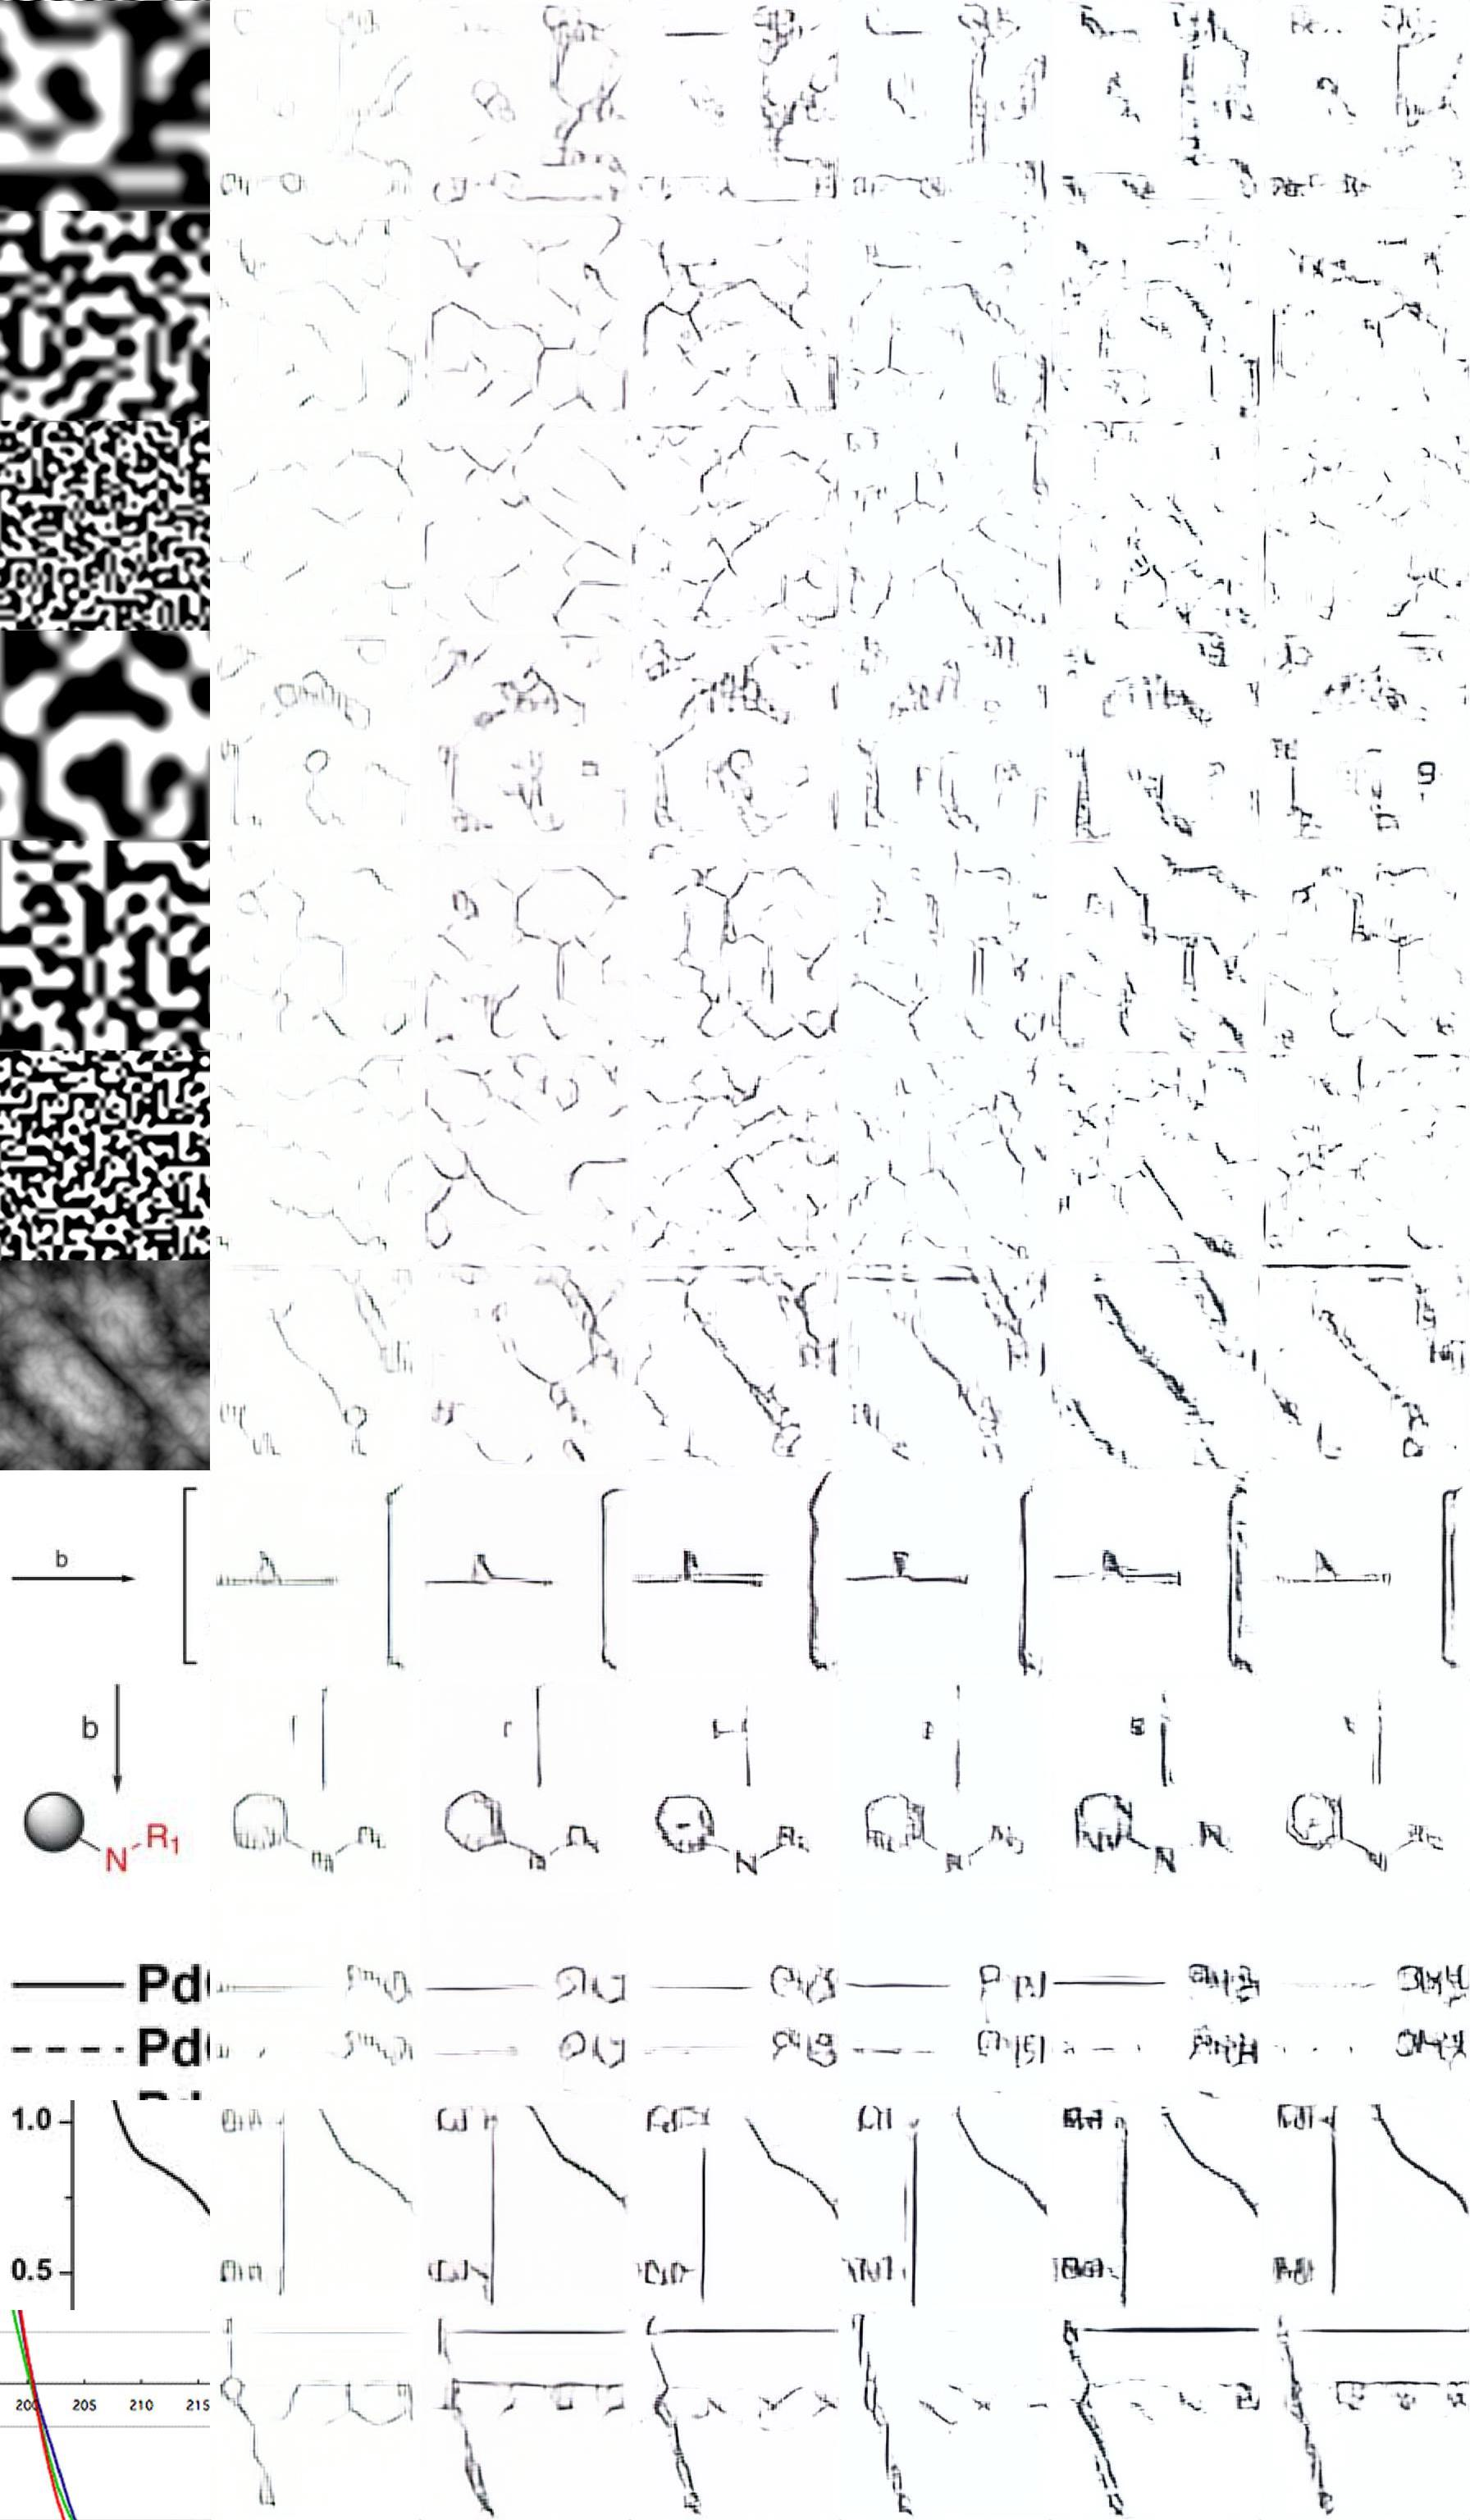
\includegraphics[scale=0.2]{imagenes/image_generation/256/256_2.jpg}}  
\end{figure}


\begin{figure}[H]
\centering
    \caption{Resultados de entrenar los modelos sobre el conjunto de datos con \textit{data augmentation} 1. La primera columna representa la imagen de entrada, el resto los diferentes modelos entrenados desde 70 hasta 170 épocas, tomadas de 20 en 20.} 
    \fbox{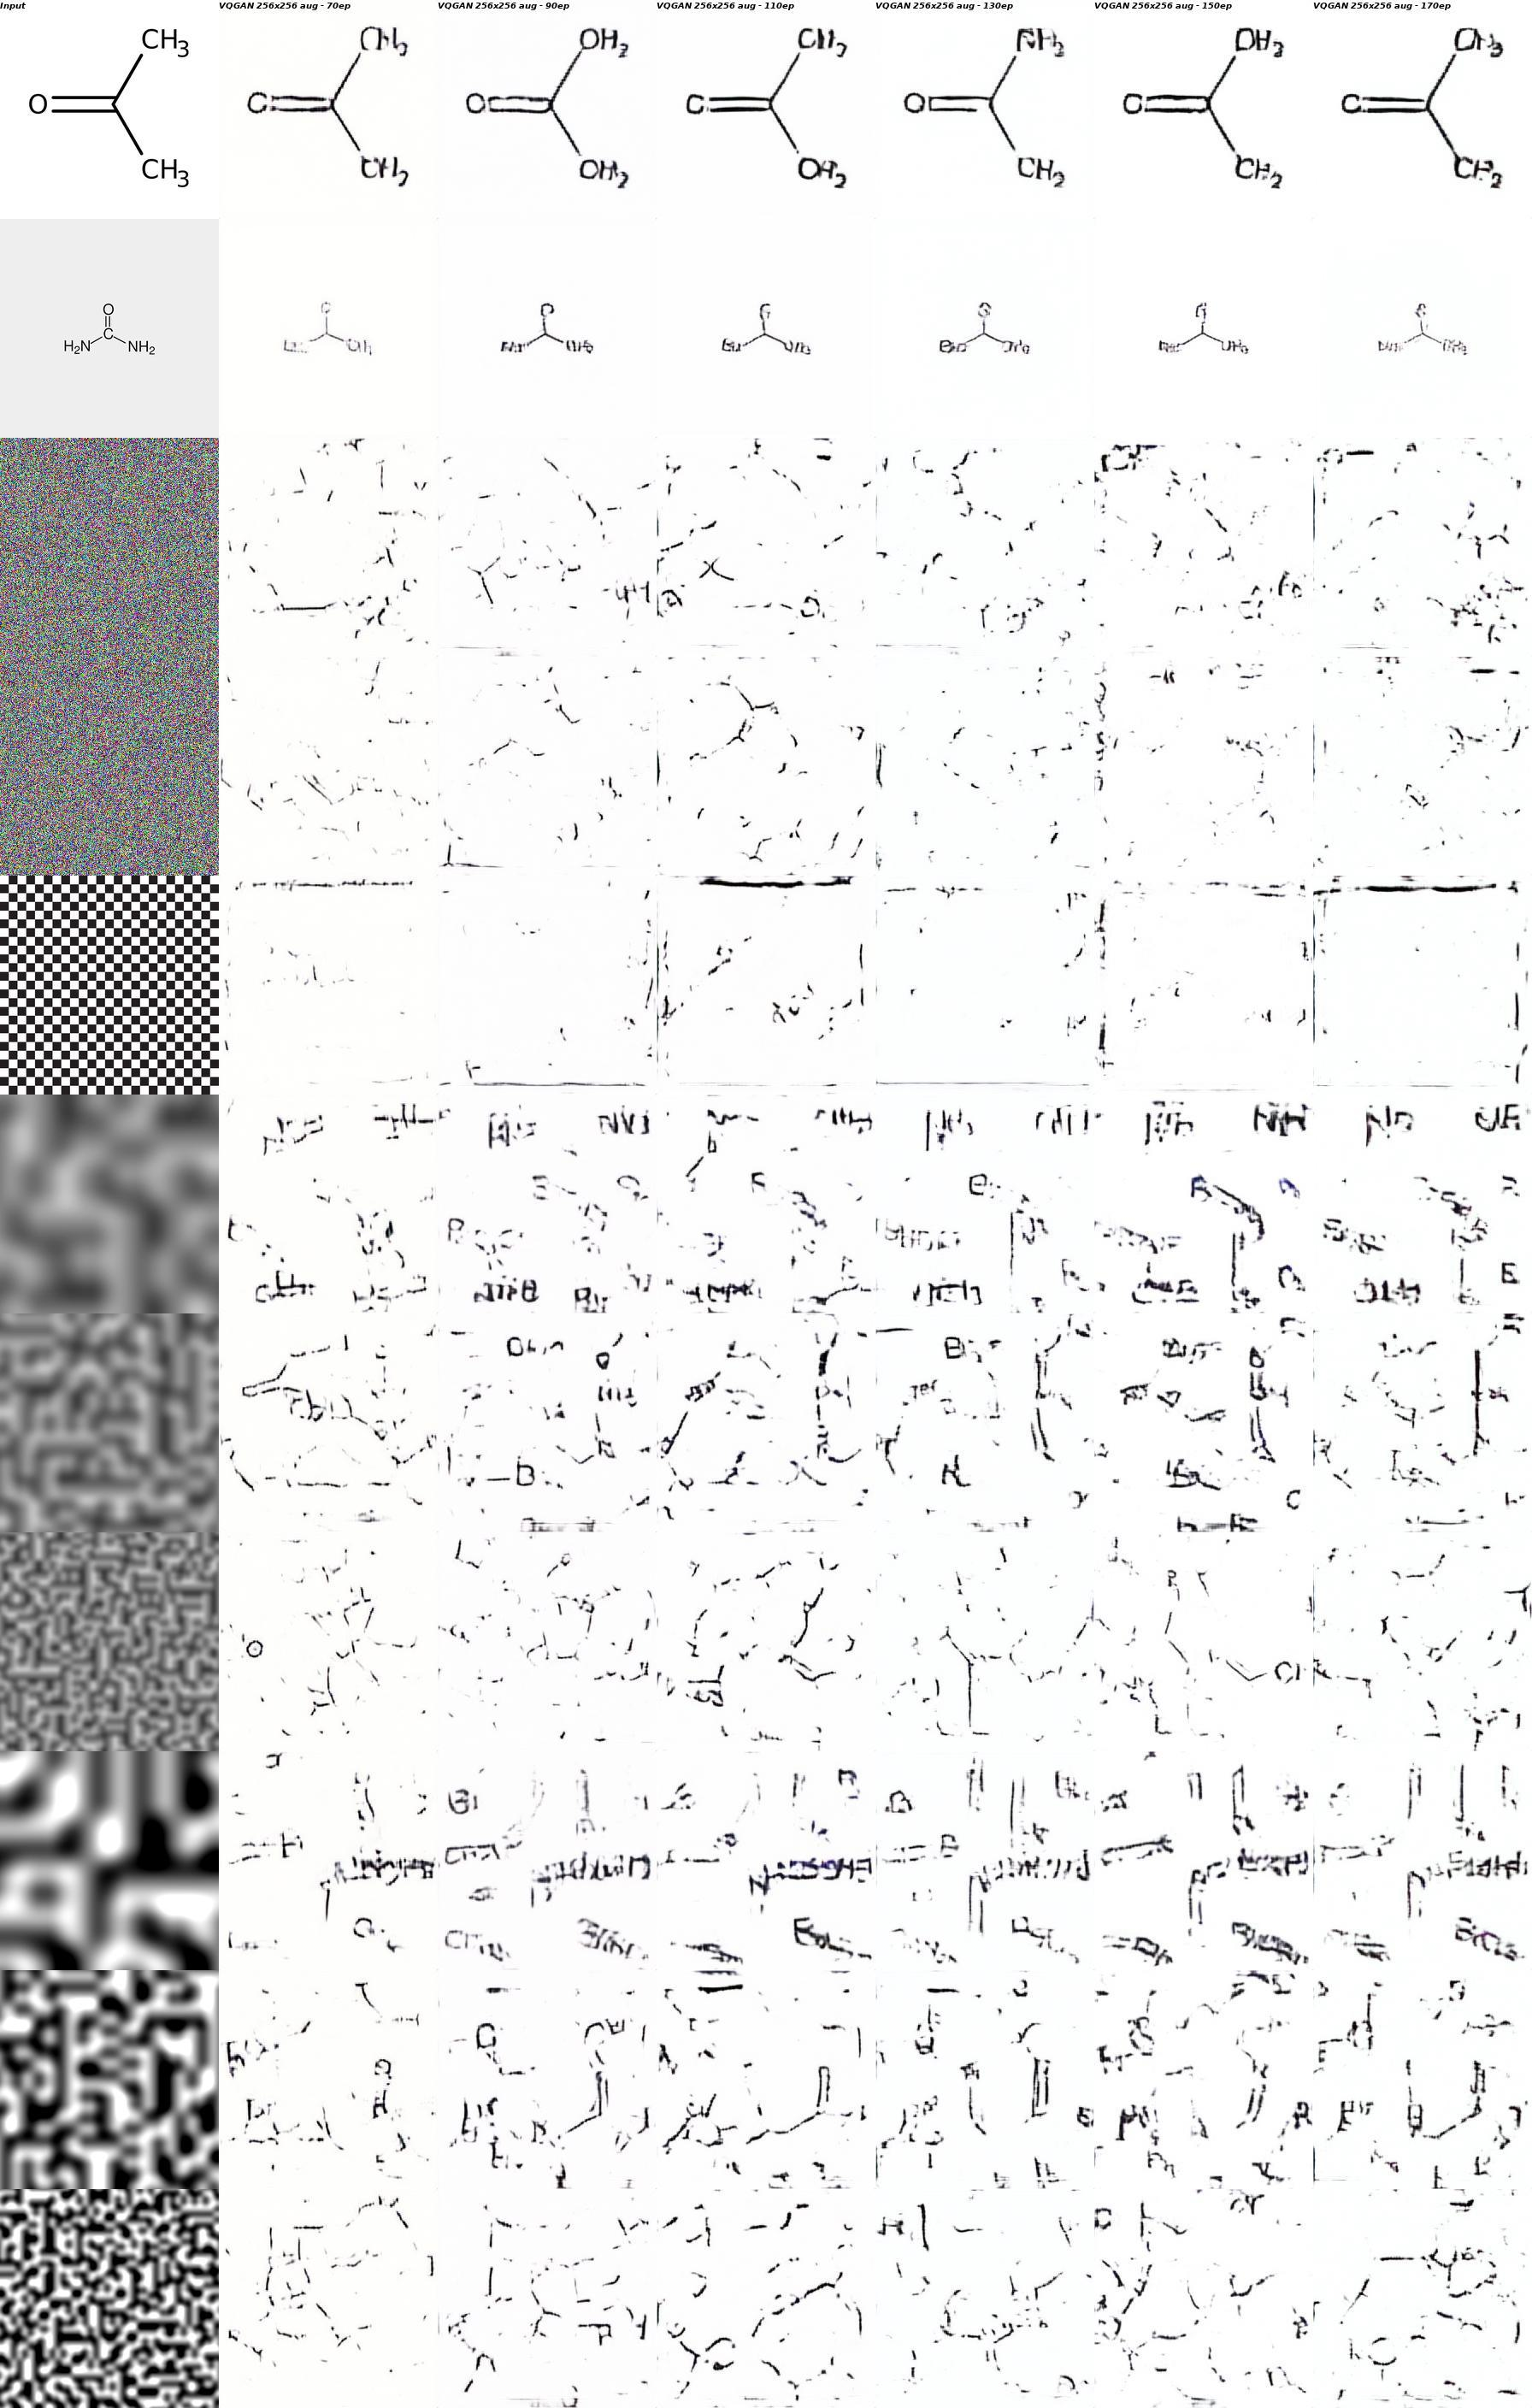
\includegraphics[scale=0.2]{imagenes/image_generation/256/aug_1.jpg}}  
    \label{fig:synthetic_molecules_aug1}
\end{figure}

\begin{figure}[H]
\centering
    \fbox{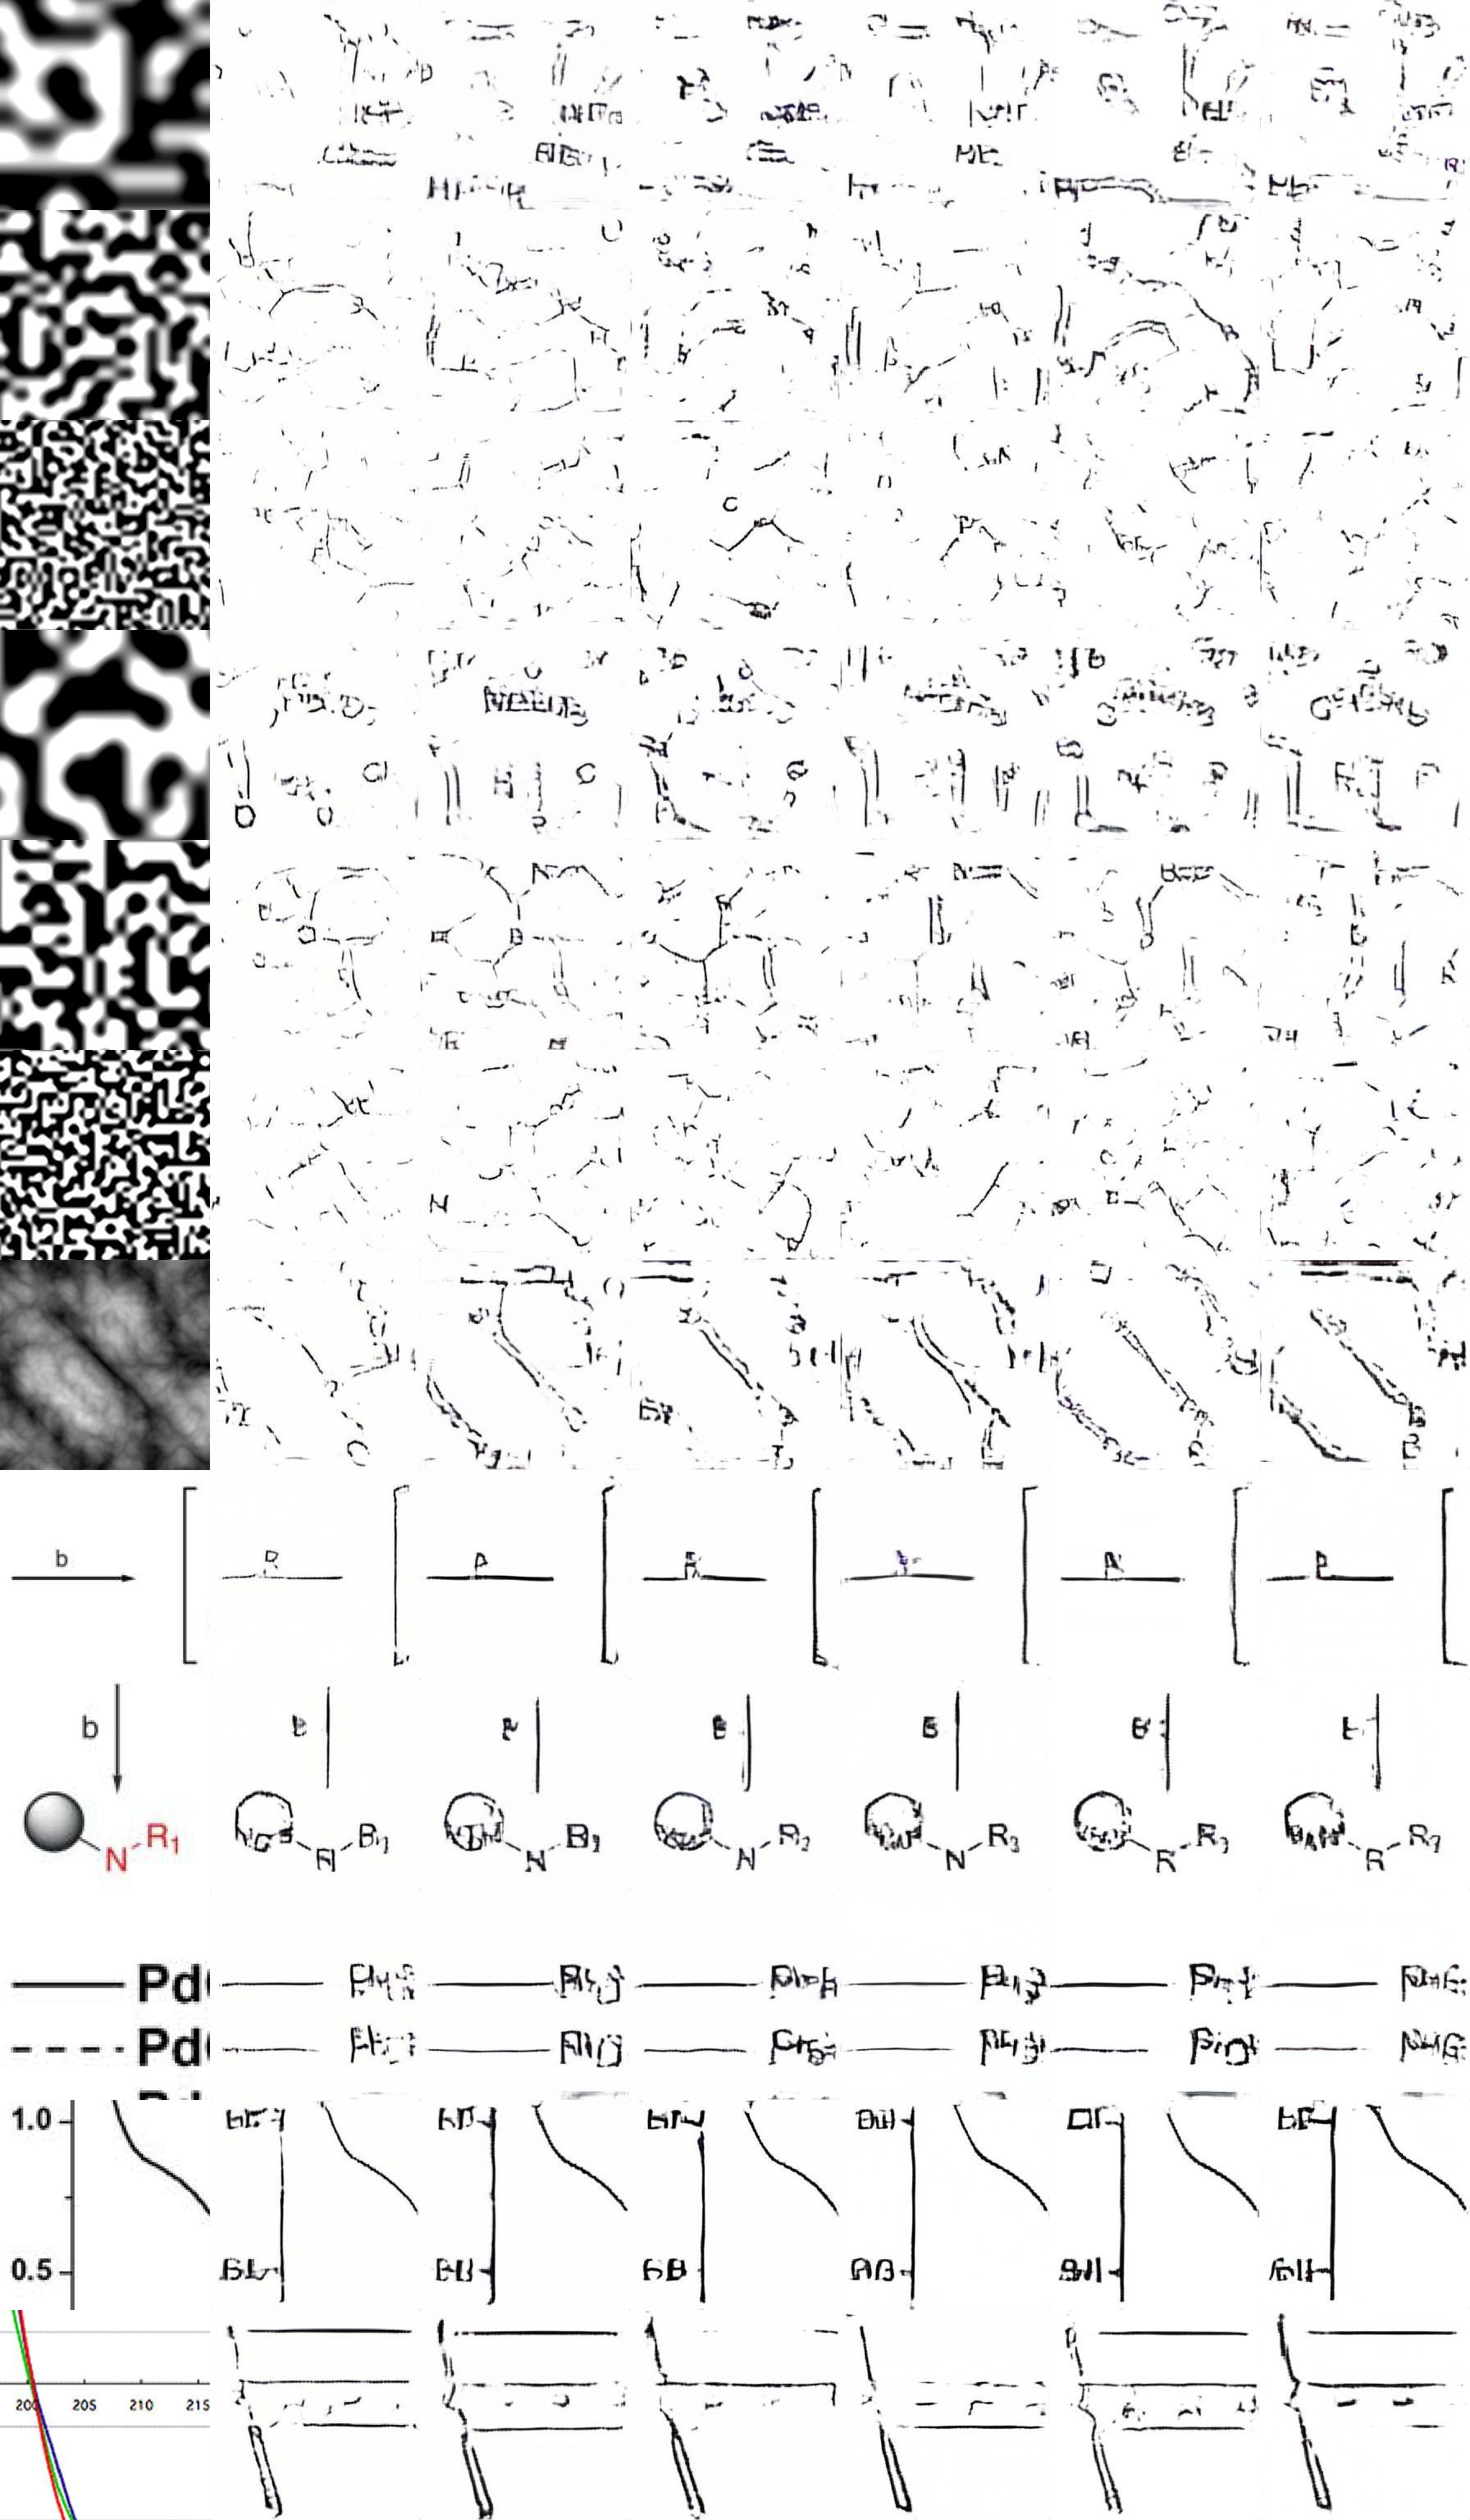
\includegraphics[scale=0.2]{imagenes/image_generation/256/aug_2.jpg}}  
\end{figure}


\begin{figure}[H]
\centering
    \caption{Resultados de entrenar los modelos sobre el conjunto de datos con \textit{data augmentation} 2. La primera columna representa la imagen de entrada, el resto los diferentes modelos entrenados desde 70 hasta 170 épocas, tomadas de 20 en 20.} 
    \fbox{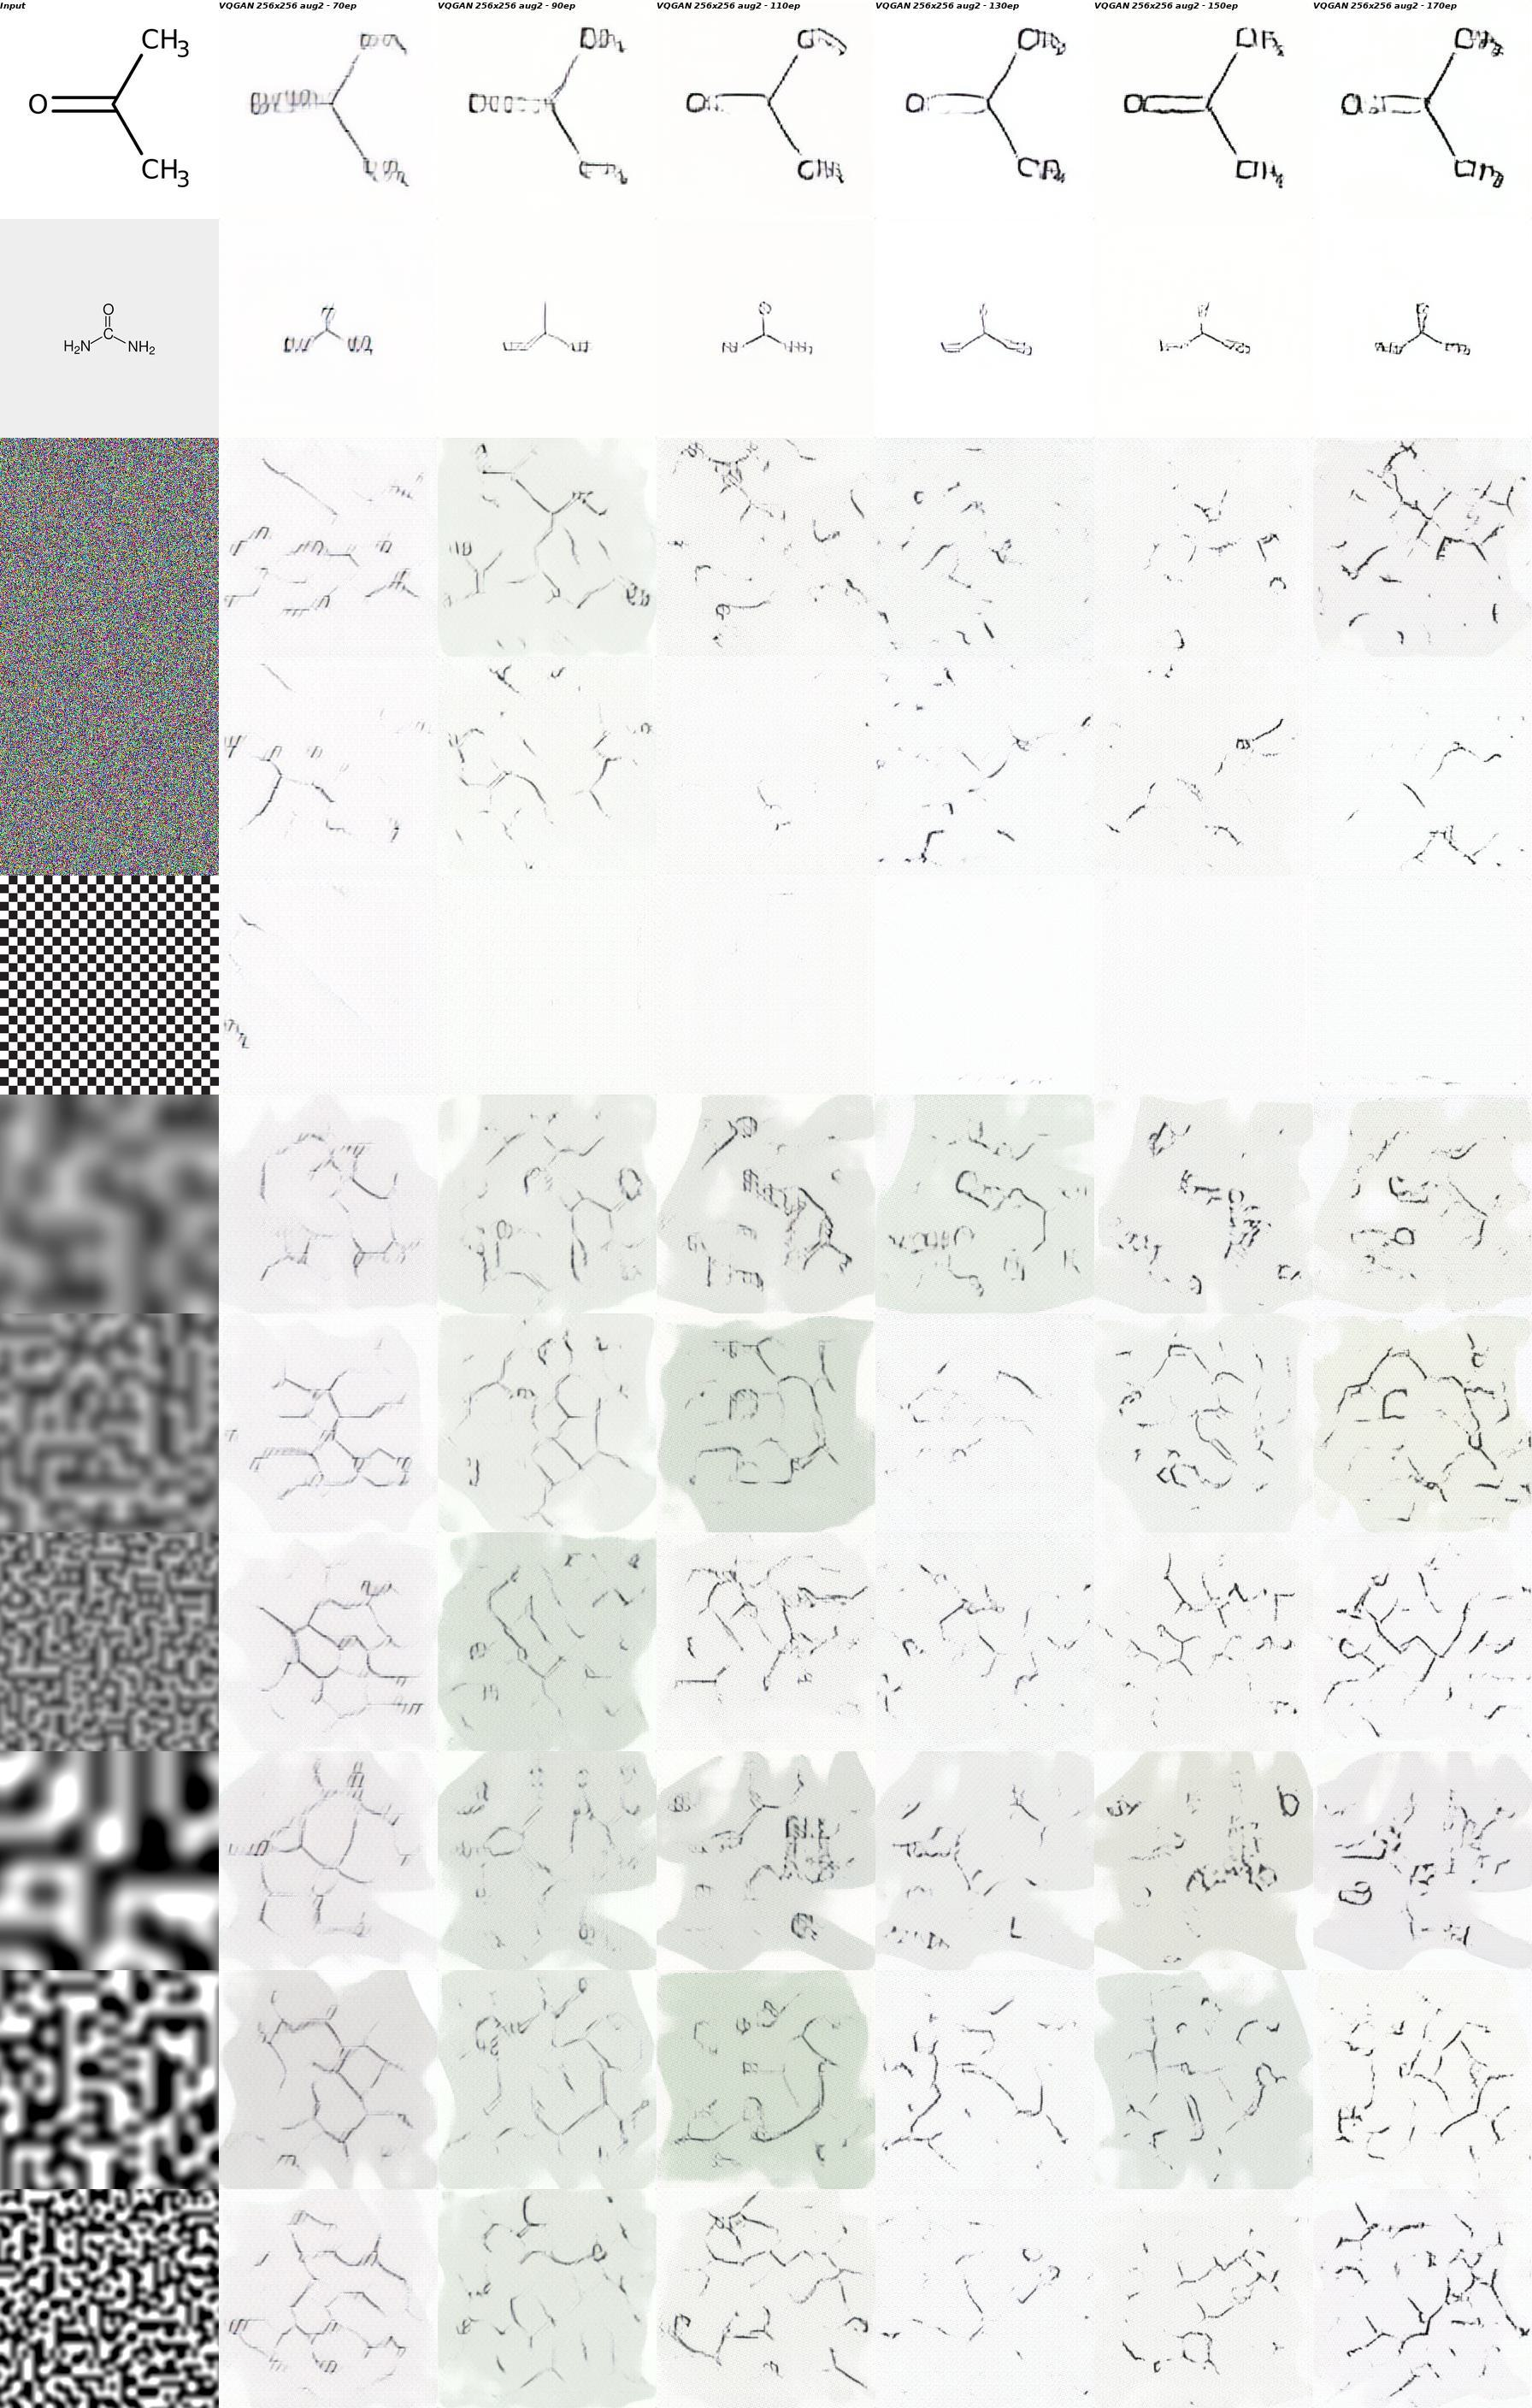
\includegraphics[scale=0.2]{imagenes/image_generation/256/aug2_1.jpg}} 
    \label{fig:synthetic_molecules_aug2} 
\end{figure}

\begin{figure}[H]
\centering
    \fbox{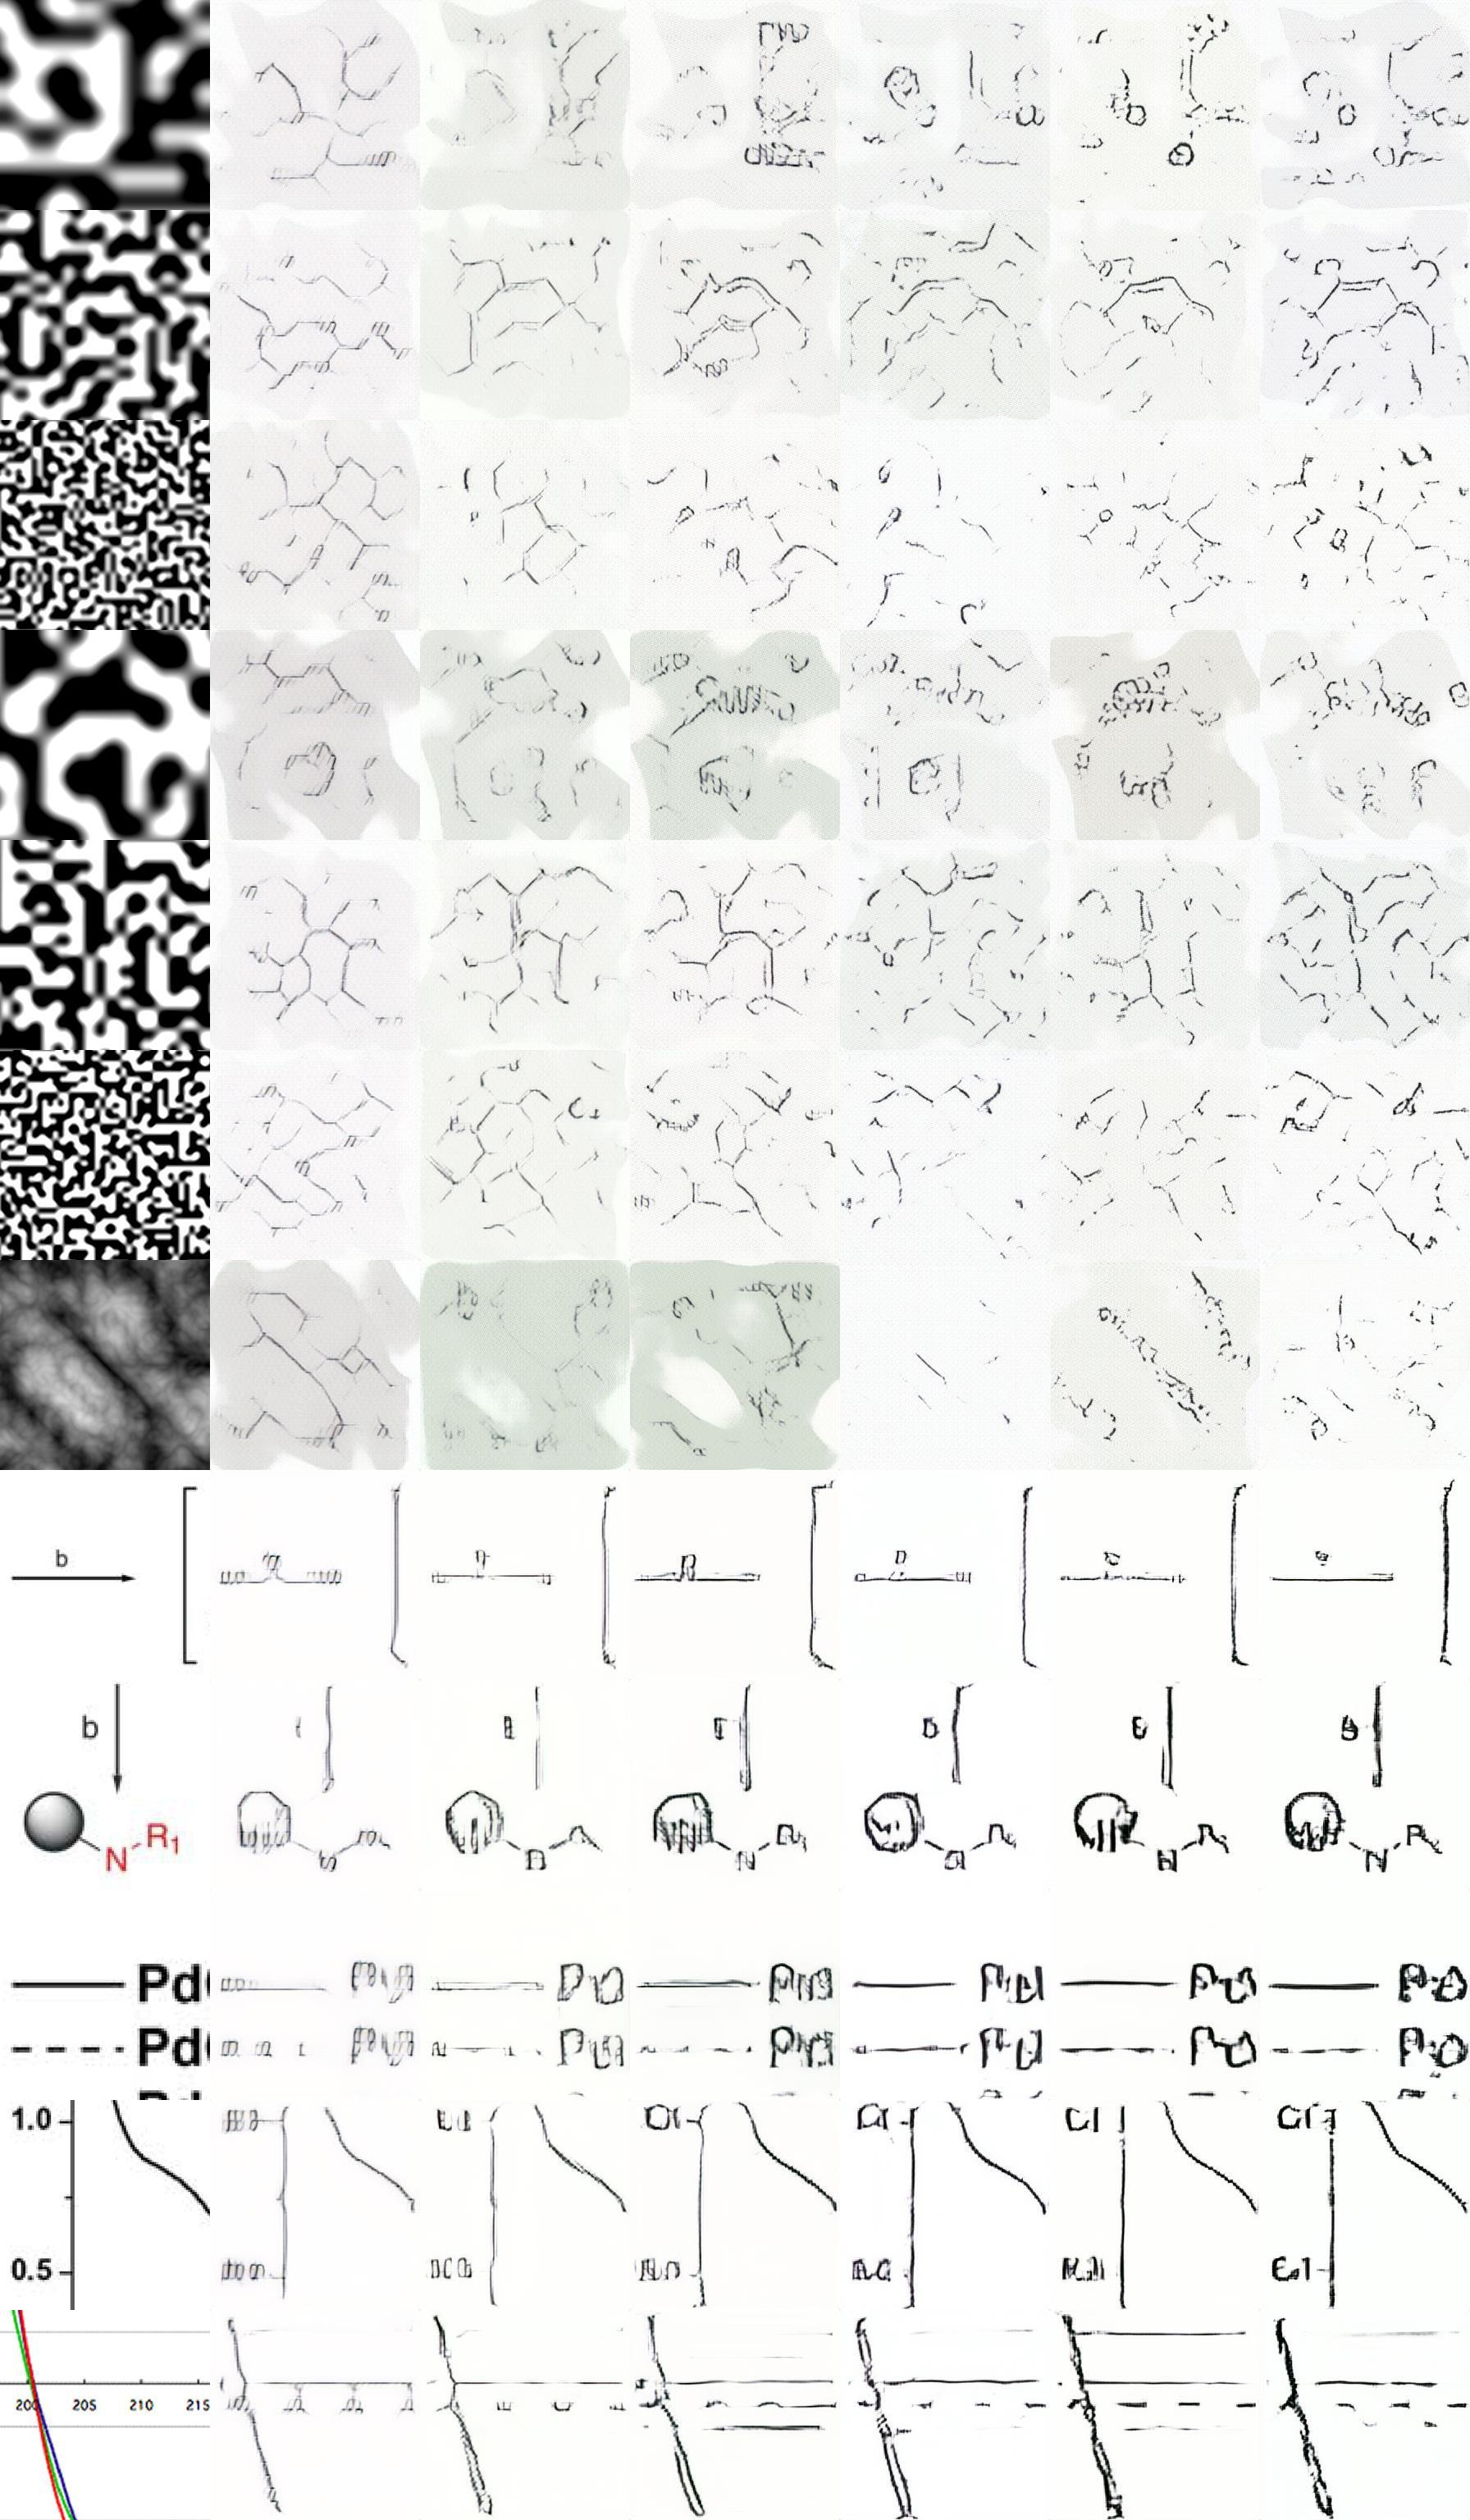
\includegraphics[scale=0.2]{imagenes/image_generation/256/aug2_2.jpg}}  

\end{figure}


\begin{figure}[H]
\centering
    \caption{Resultados de entrenar los modelos sobre el conjunto de datos con \textit{data augmentation} 3. La primera columna representa la imagen de entrada, el resto los diferentes modelos entrenados desde 70 hasta 170 épocas, tomadas de 20 en 20.}
    \fbox{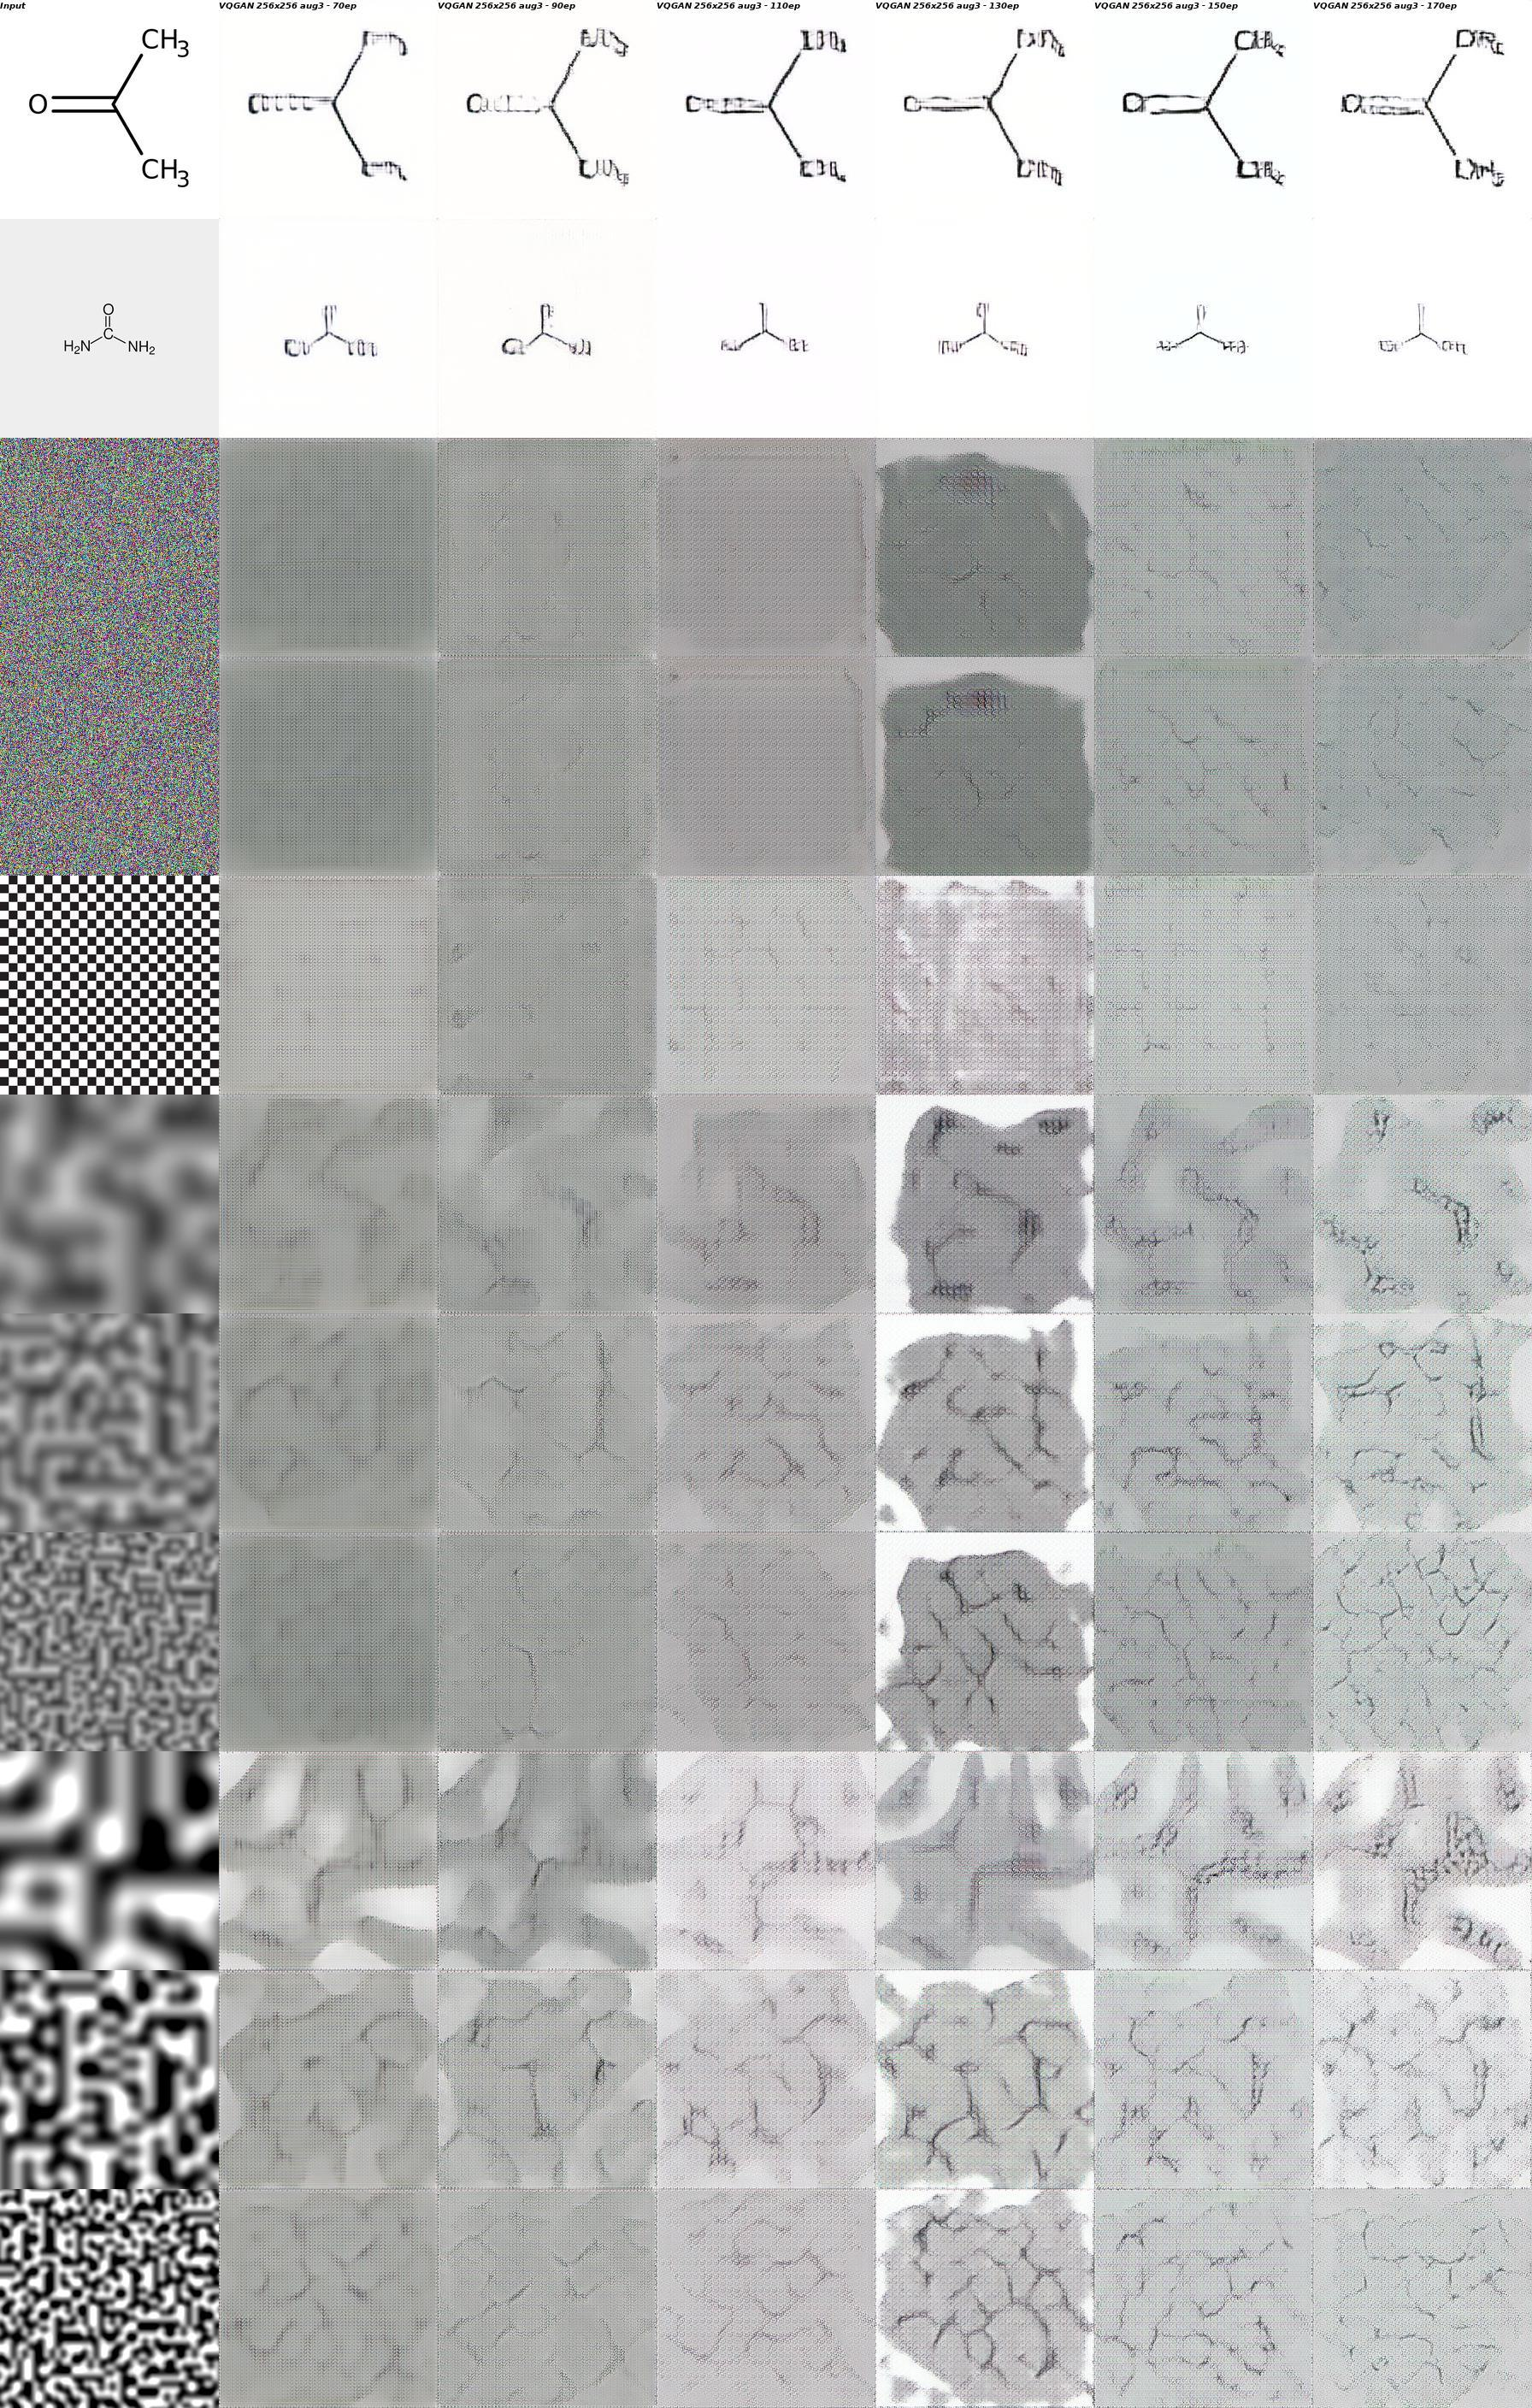
\includegraphics[scale=0.2]{imagenes/image_generation/256/aug3_1.jpg}}  
    \label{fig:synthetic_molecules_aug3}
\end{figure}

\begin{figure}[H]
\centering
    \fbox{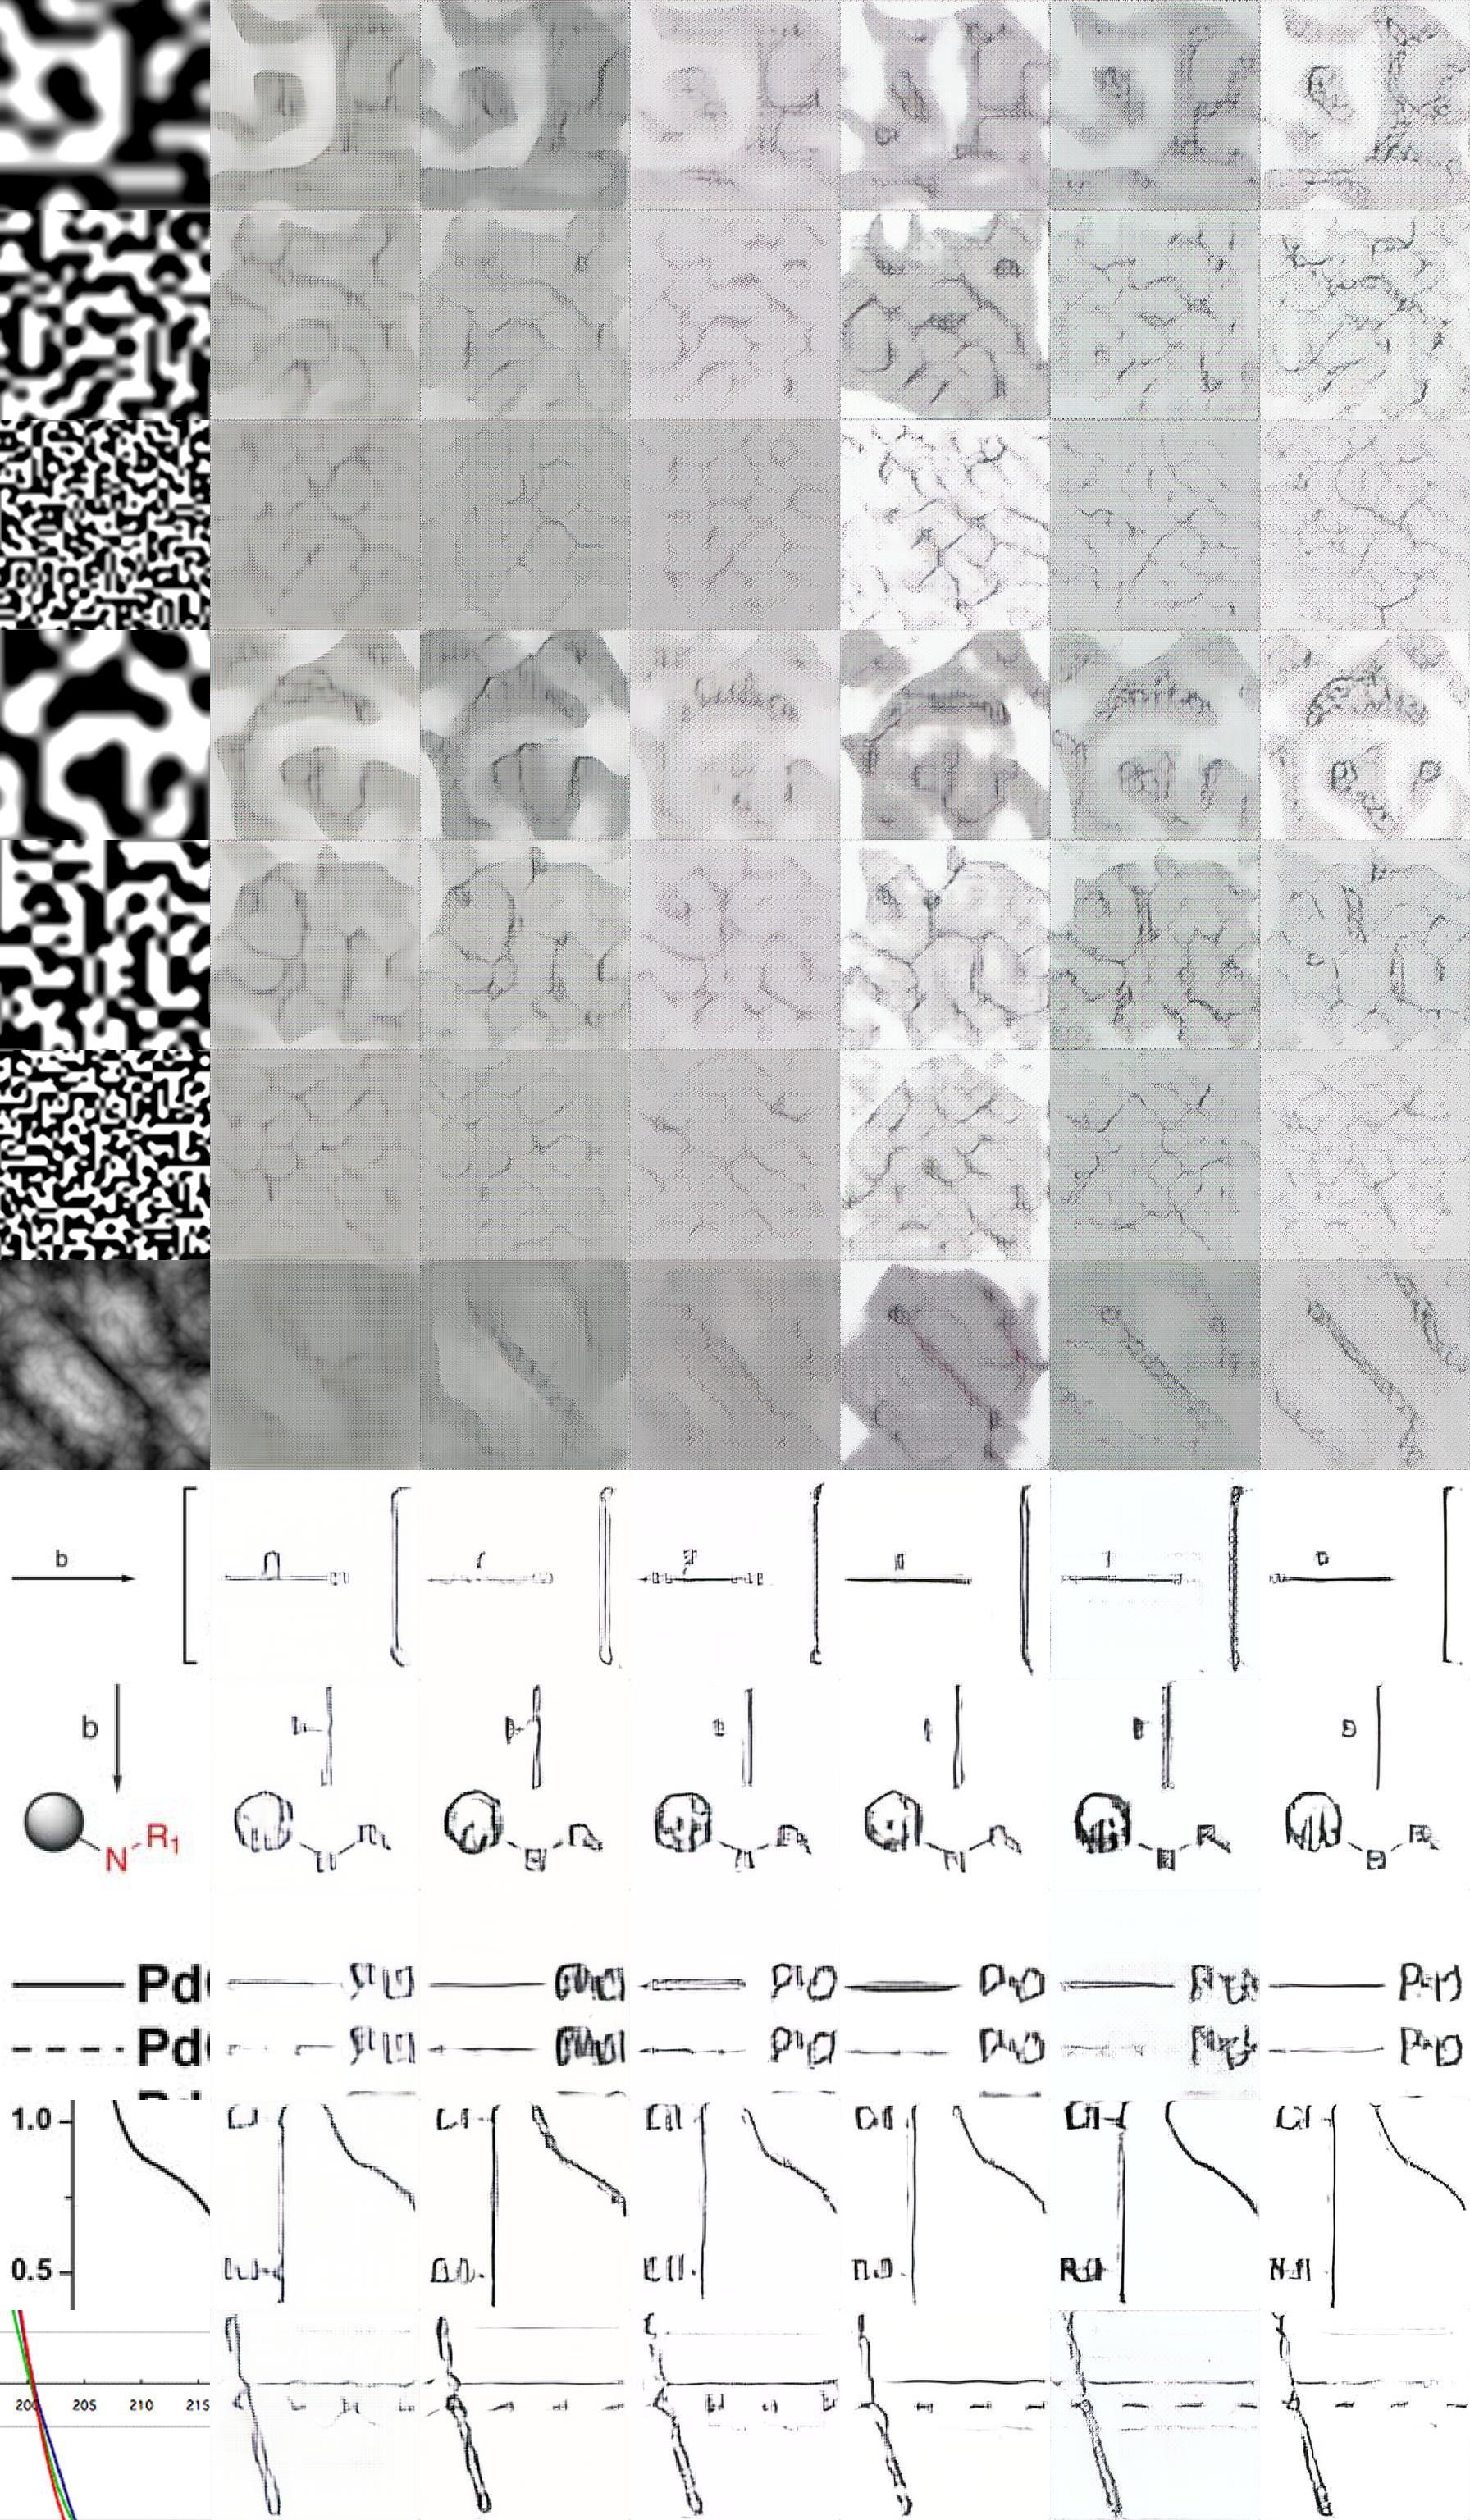
\includegraphics[scale=0.2]{imagenes/image_generation/256/aug3_2.jpg}}  
\end{figure}

¿Qué tipo de datos de entrada se han utilizado para generar las imágenes sintéticas? En un primer momento se ha probado a utilizar imágenes de moléculas reales y de objetos que, sin ser moléculas, lo parecen. En el primer caso, la salida es similar a la entrada, con la diferencia de que la imagen sintética pierde información: detalles como letras o números se alteran. En el segundo caso ocurre algo similar, con la particularidad de que objetos circulares son transformados en formas que parecen hexágonos propios de las moléculas. Además, incluso se añaden átomos (Figura \ref{fig:circle-hex}).

\begin{figure}[H]
\centering
    \fbox{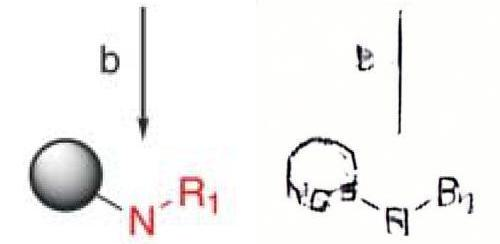
\includegraphics[scale=0.3]{imagenes/image_generation/256/circle_to_hex.jpg}}
    \caption{El modelo tiene la capacidad de modificar la imagen para que se parezca a una molécula.}
    \label{fig:circle-hex}
\end{figure}

Pero se quiere poder generar tantas imágenes como sean necesarias, así que se debería poder partir de una imagen de entrada generada aleatoriamente. En un primer momento se utilizó ruido uniforme, pero no funcionó bien en ningún caso. Este tipo de ruido no sigue ninguna estructura, y nuestro modelo necesita una entrada que tenga cierta continuidad. Por ello pruebo con una cuadrícula de ajedrez: ocurre lo mismo, ya que aunque existe un patrón que se repite, los elementos de este no están conectados entre sí.

\subsection{Ruido Perlín}
Se trata de un ruido inventado por Ken Perlín en 1982 que revolucionó el ámbito de la Informática Gráfica. En esta rama de las Ciencias de la Computación, la creación de texturas que imitan materiales de la naturaleza como la madera o el mármol es una tarea importante. Generar estas texturas de una forma manual o mediante un escáner no es una opción escalable.

Este ruido permite simular fenómenos que requieran aleatoriedad a la vez que continuidad. Para ello, genera una serie de gradientes en un \textit{grid} (en nuestro caso 2D). A continuación, interpola el valor de esos gradientes mediante interpolación polinómica de Hermite (Figura \ref{fig:interpolacion}). La ventaja de este ruido frente a otros que también se generan mediante interpolación es su eficiencia, para calcular la interpolación en un punto solo intervienen los $2^n$ gradientes más cercanos, donde $n$ es el número de dimensiones. \cite{computer-graphics-epfl}

\begin{figure}[H]
\centering
    \fbox{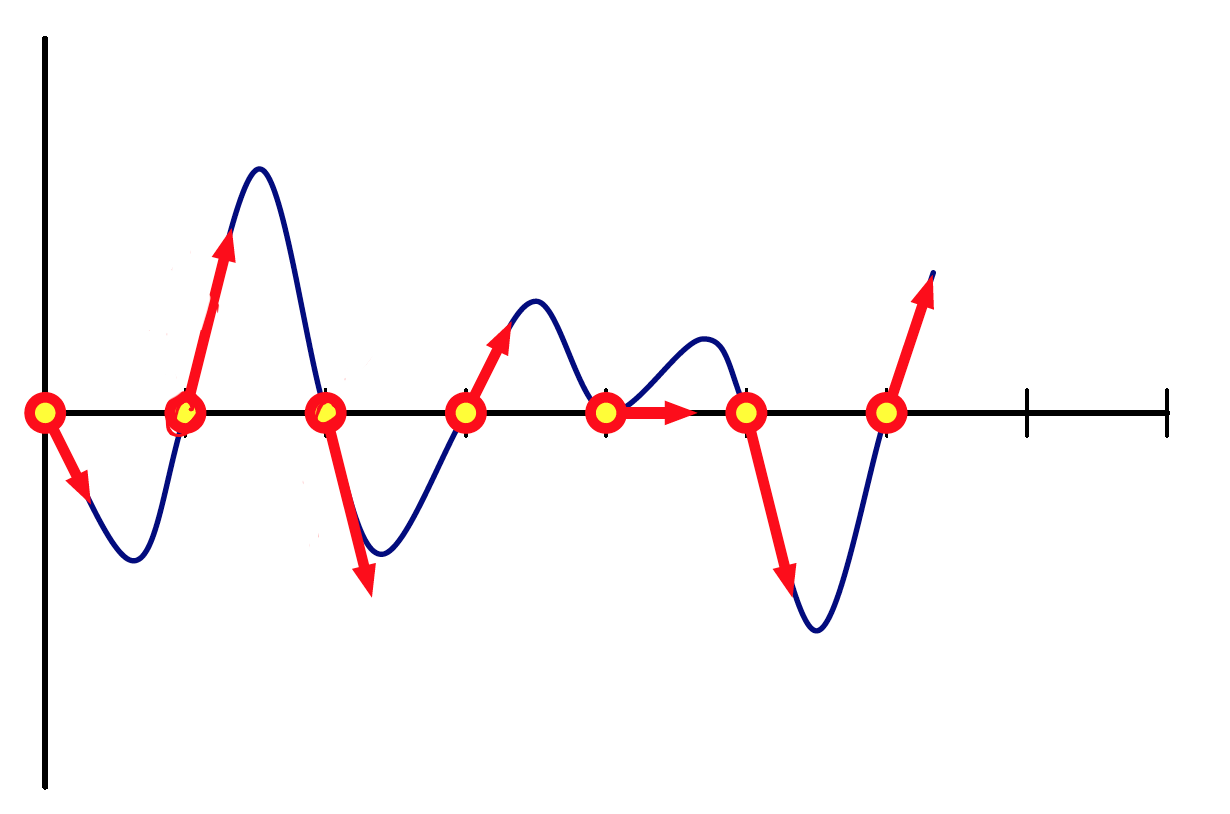
\includegraphics[scale=0.3]{imagenes/image_generation/perlin_interpolation.png}}
    \caption{Interpolación de gradientes en el Ruido Perlín 1D. \cite{computer-graphics-epfl}}
    \label{fig:interpolacion}
\end{figure}

El Ruido Perlín se puede modificar cambiando la amplitud y frecuencia de este. A mayor amplitud, los cambios entre zonas del ruido serán más bruscos, a menor amplitud el ruido será más homogéneo y suave. La frecuencia cambia la granularidad del ruido, a mayor frecuencia encontramos un grano más fino. 

\begin{figure}[H]
\centering
    \begin{subfigure}{.26\textwidth}
        \centering
        
\includegraphics[width=1\linewidth]{imagenes/image_generation/perlin_python_3_1.jpg}
        \caption{Amp:3 Frec:1}
    \end{subfigure}%
    \begin{subfigure}{.26\textwidth}
        \centering
        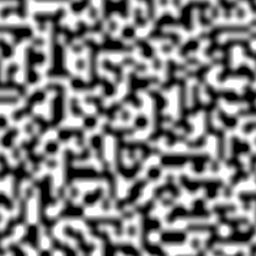
\includegraphics[width=1\linewidth]{imagenes/image_generation/perlin_python_3_4.jpg}
        \caption{Amp:3 Frec:4}
    \end{subfigure}%

    \bigskip

    \begin{subfigure}{.26\textwidth}
        \centering
        
\includegraphics[width=1\linewidth]{imagenes/image_generation/perlin_python_7_1.jpg}
        \caption{Amp:7 Frec:1}
    \end{subfigure}%
    \begin{subfigure}{.26\textwidth}
        \centering
        
\includegraphics[width=1\linewidth]{imagenes/image_generation/perlin_python_7_4.jpg}
        \caption{Amp:7 Frec:4}
    \end{subfigure}

    \caption{Ejemplos de Ruido Perlín con distinta amplitud y frecuencia.}
\end{figure}

Como se observa en las figuras \ref{fig:synthetic_molecules}, \ref{fig:synthetic_molecules_aug1}, \ref{fig:synthetic_molecules_aug2} y \ref{fig:synthetic_molecules_aug3}, al contrario que con el ruido uniforme, este tipo de ruido es capaz de generar imágenes que parecen moléculas. Su continuidad permite que el modelo tenga una estructura en la que basarse para realizar la generación. 

Tras realizar estos experimentos, se los mostré al equipo para conocer su opinión: está conforme con la versión \textit{data augmentation} 2 entrenada durante 70 épocas en aquellos casos en los que se utiliza Ruido Perlín como entrada (figural \ref{fig:synthetic_molecules_aug2}, segunda columna). De todas formas, como se obtienen buenos resultados entre 70 y 90 épocas, voy a entrenar con \textit{data augmentation} 2 durante 70, 75, 80, 85 y 90 épocas y a comparar los resultados.

\begin{figure}[H]
\centering
    \caption{Resultados de entrenar con imágenes con \textit{data augmentation} 2. La primera columna representa la imagen de entrada (ruido Perlín en todos los casos), el resto los diferentes modelos entrenados desde las 70 hasta las 90 épocas tomadas de 5 en 5.}
    \fbox{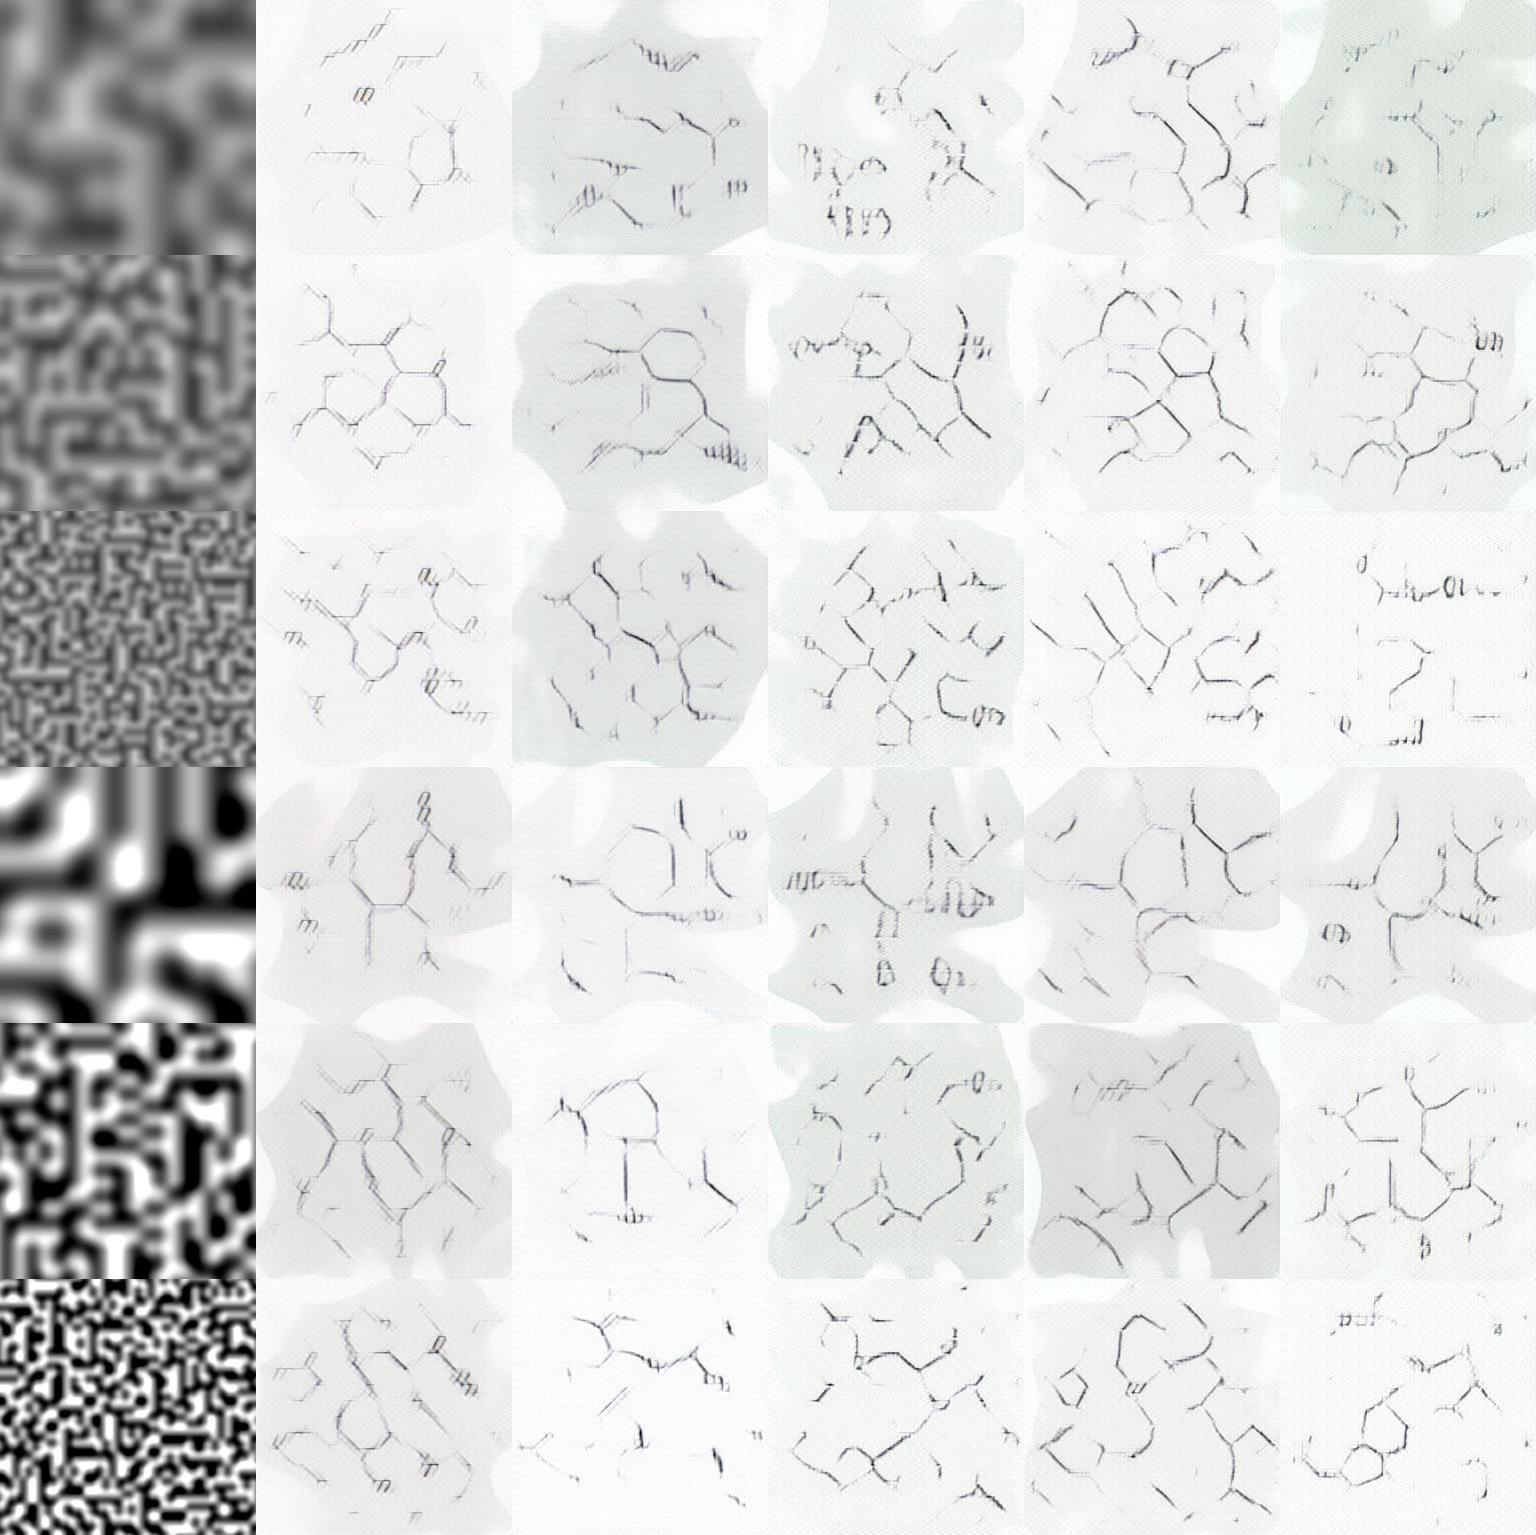
\includegraphics[scale=0.23]{imagenes/image_generation/256/aug2_extraepochs_1.jpg}}  
    \label{fig:synthetic_molecules_aug2_extra} 
\end{figure}

\begin{figure}[H]
\centering
    \fbox{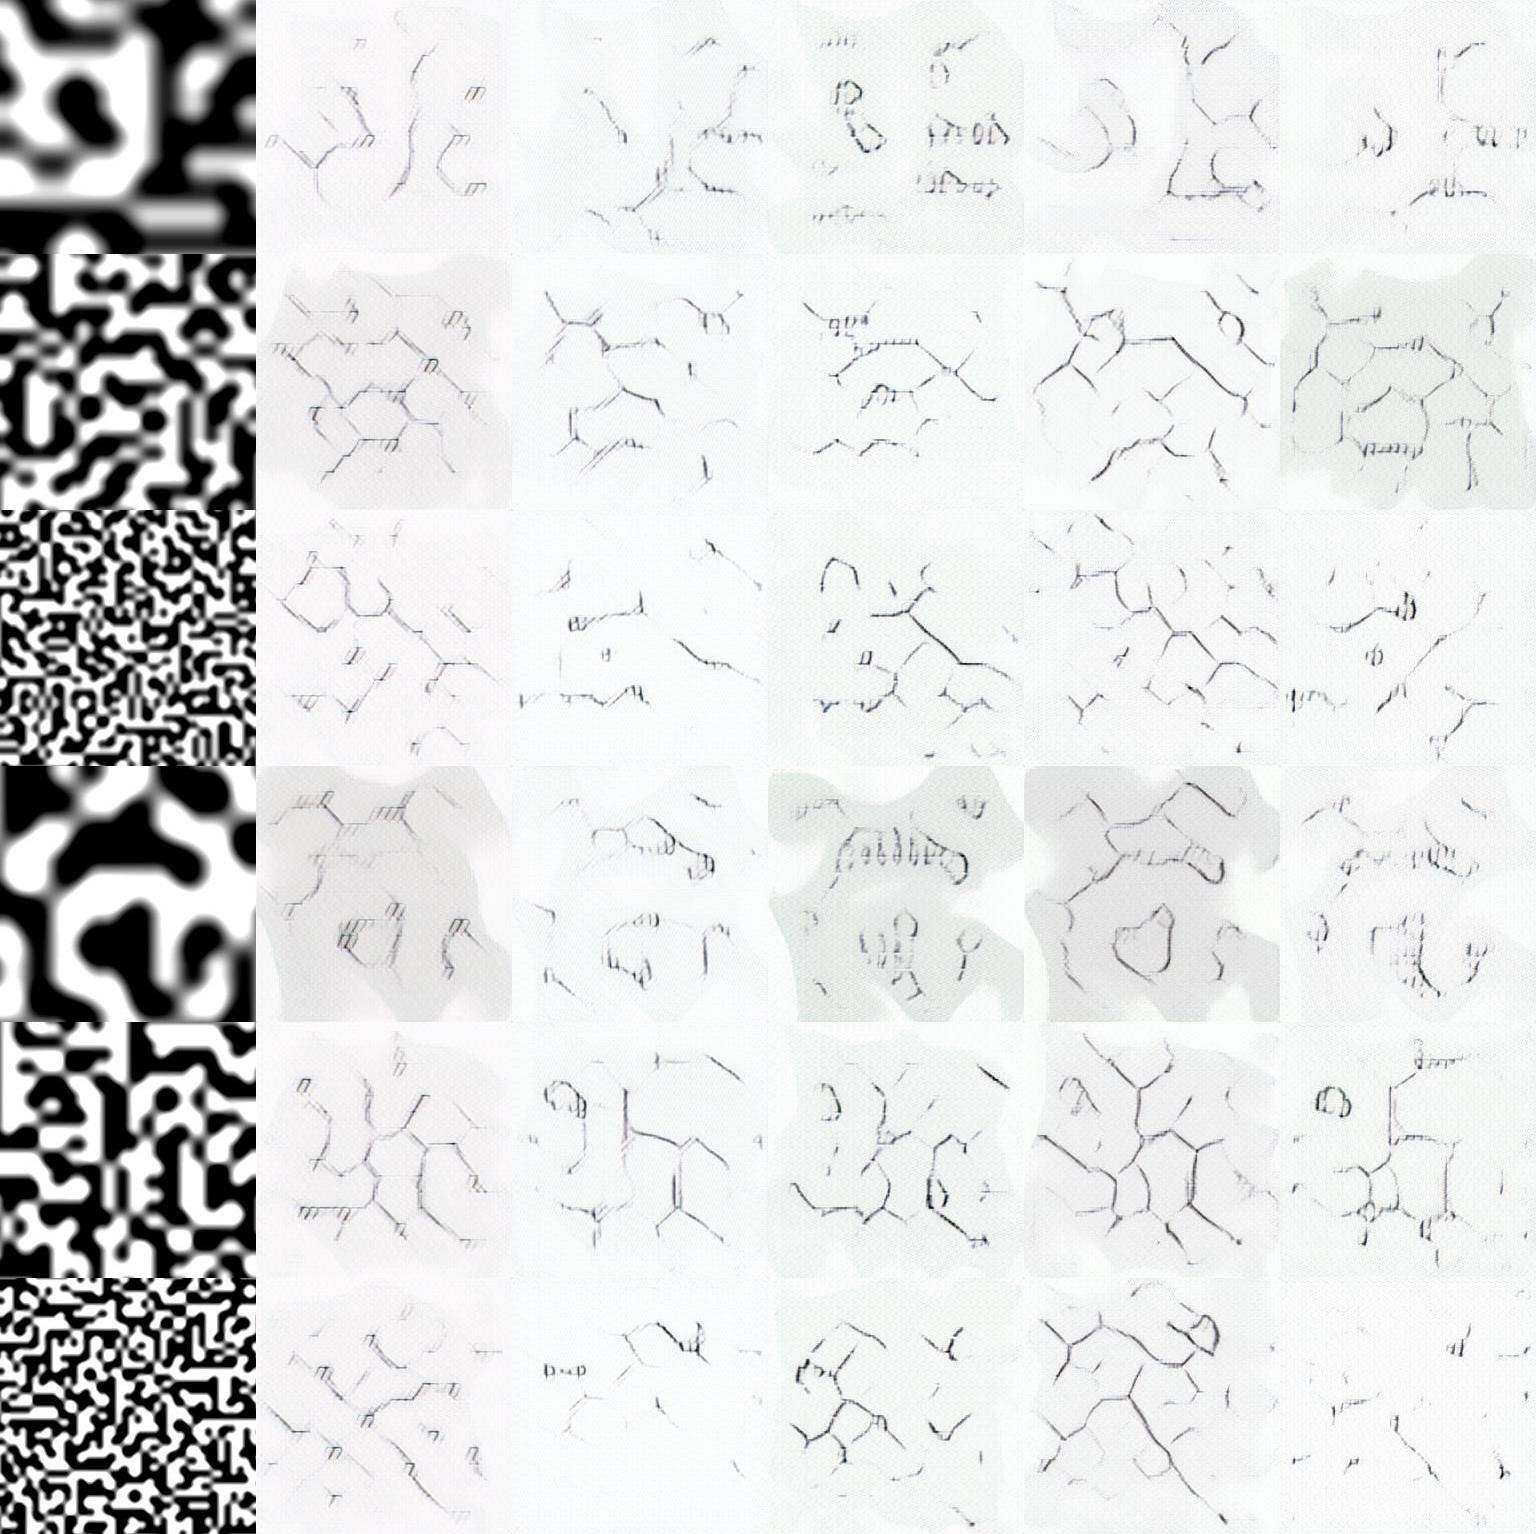
\includegraphics[scale=0.23]{imagenes/image_generation/256/aug2_extraepochs_2.jpg}}  
\end{figure}

En diferente número de épocas/tipos de ruido Perlín se obtienen buenos resultados, por lo que no voy a utilizar una única configuración para generar los \textit{hard negatives}, se utilizarán varias hasta alcanzar los 400 que quiero generar. 

En concreto, voy a obtener 50 imágenes a partir de cada una de estas configuraciones (todas ellas obtenidas tras entrenar sobre \textit{data augmentation} 2):

\begin{itemize}
    \item Modelo entrenado durante 70 épocas al que se le introduce ruido Perlín con amplitud 1 y frecuencia 2 (fila 2 columna 2 de la figura \ref{fig:synthetic_molecules_aug2_extra}).
    \item Modelo entrenado durante 70 épocas al que se le introduce ruido Perlín con amplitud 1 y frecuencia 4 (fila 3 columna 2 de la figura \ref{fig:synthetic_molecules_aug2_extra}).
    \item Modelo entrenado durante 70 épocas al que se le introduce ruido Perlín con amplitud 3 y frecuencia 2 (fila 5 columna 2 de la figura \ref{fig:synthetic_molecules_aug2_extra}).
    \item Modelo entrenado durante 75 épocas al que se le introduce ruido Perlín con amplitud 1 y frecuencia 4 (fila 3 columna 3 de la figura \ref{fig:synthetic_molecules_aug2_extra}).
    \item Modelo entrenado durante 75 épocas al que se le introduce ruido Perlín con amplitud 3 y frecuencia 2 (fila 5 columna 3 de la figura \ref{fig:synthetic_molecules_aug2_extra}).
    \item Modelo entrenado durante 80 épocas al que se le introduce ruido Perlín con amplitud 1 y frecuencia 2 (fila 2 columna 4 de la figura \ref{fig:synthetic_molecules_aug2_extra}).
    \item Modelo entrenado durante 85 épocas al que se le introduce ruido Perlín con amplitud 1 y frecuencia 2 (fila 2 columna 5 de la figura \ref{fig:synthetic_molecules_aug2_extra}).
    \item Modelo entrenado durante 85 épocas al que se le introduce ruido Perlín con amplitud 7 y frecuencia 2 (fila 11 columna 5 de la figura \ref{fig:synthetic_molecules_aug2_extra}).
\end{itemize}

En total, 400 \textit{hard negatives}. Antes de unificarlos con 400 ejemplos negativos del \textit{dataset} original, los trato de forma que se reduce el color grisáceo de fondo que presentan tras ser producidos por los modelos generadores. Para ello, de forma independiente en cada una de las configuraciones, fijo un umbral de color que, si no es superado por un pixel, este es transformado en color blanco. De esta forma, solo los píxeles con un color intenso se mantienen en la imagen, o sea, solo se mantiene la estructura molecular. Antes de eso, aplico un aumento de contraste a la imagen y un filtro de apertura (\textit{opening}) que elimina ruido. Algunos ejemplos resultantes se pueden observar en la Figura \ref{fig:hard-negatives}.

\begin{figure}[H]
\centering
    \begin{subfigure}{.28\textwidth}
        \centering
        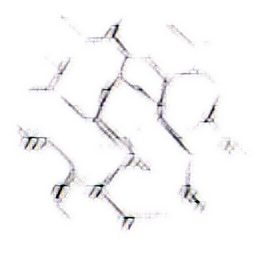
\includegraphics[width=1\linewidth]{imagenes/image_generation/clean_results/perlin_e70_a1_f2_2.jpg}
    \end{subfigure}%
    \begin{subfigure}{.28\textwidth}
        \centering
        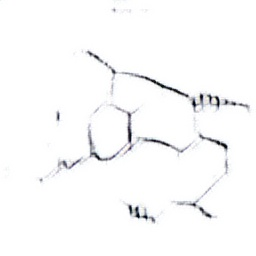
\includegraphics[width=1\linewidth]{imagenes/image_generation/clean_results/perlin_e75_a1_f4_33.jpg}
    \end{subfigure}%

    \bigskip

    \begin{subfigure}{.28\textwidth}
        \centering
        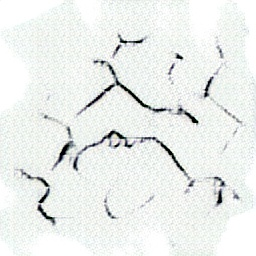
\includegraphics[width=1\linewidth]{imagenes/image_generation/clean_results/perlin_e80_a1_f2_13.jpg}
    \end{subfigure}%
    \begin{subfigure}{.28\textwidth}
        \centering
        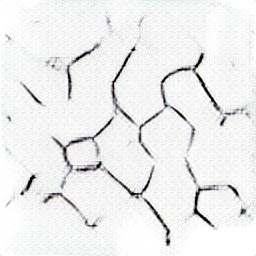
\includegraphics[width=1\linewidth]{imagenes/image_generation/clean_results/perlin_e85_a7_f2_42.jpg}
    \end{subfigure}

    \caption{\textit{Hard negatives} finales tras ser post-procesados.}
    \label{fig:hard-negatives}
\end{figure}

Ya puedo crear los dos \textit{datasets} finales para entrenar el clasificador, tal y como se expone en la Figura \ref{fig:two_final_datasets} del capítulo anterior.

\newpage
Otra prueba que se hizo y fue descartada consistió en entrenar el modelo generador a partir de ejemplos negativos. Si, en vez de entrenar sobre ejemplos positivos como estaba haciendo hasta ahora, hacerlo sobre negativos. ¿Qué ocurrió? Como se puede observar en la Figura \ref{fig:extraepochs}, los resultados no fueron buenos.

\begin{figure}[H]
\centering
    \caption{Resultados de entrenar con ejemplos negativos. La primera columna representa la imagen de entrada, el resto los diferentes modelos entrenados desde las 70 hasta las 170 épocas tomadas de 20 en 20.}
    \fbox{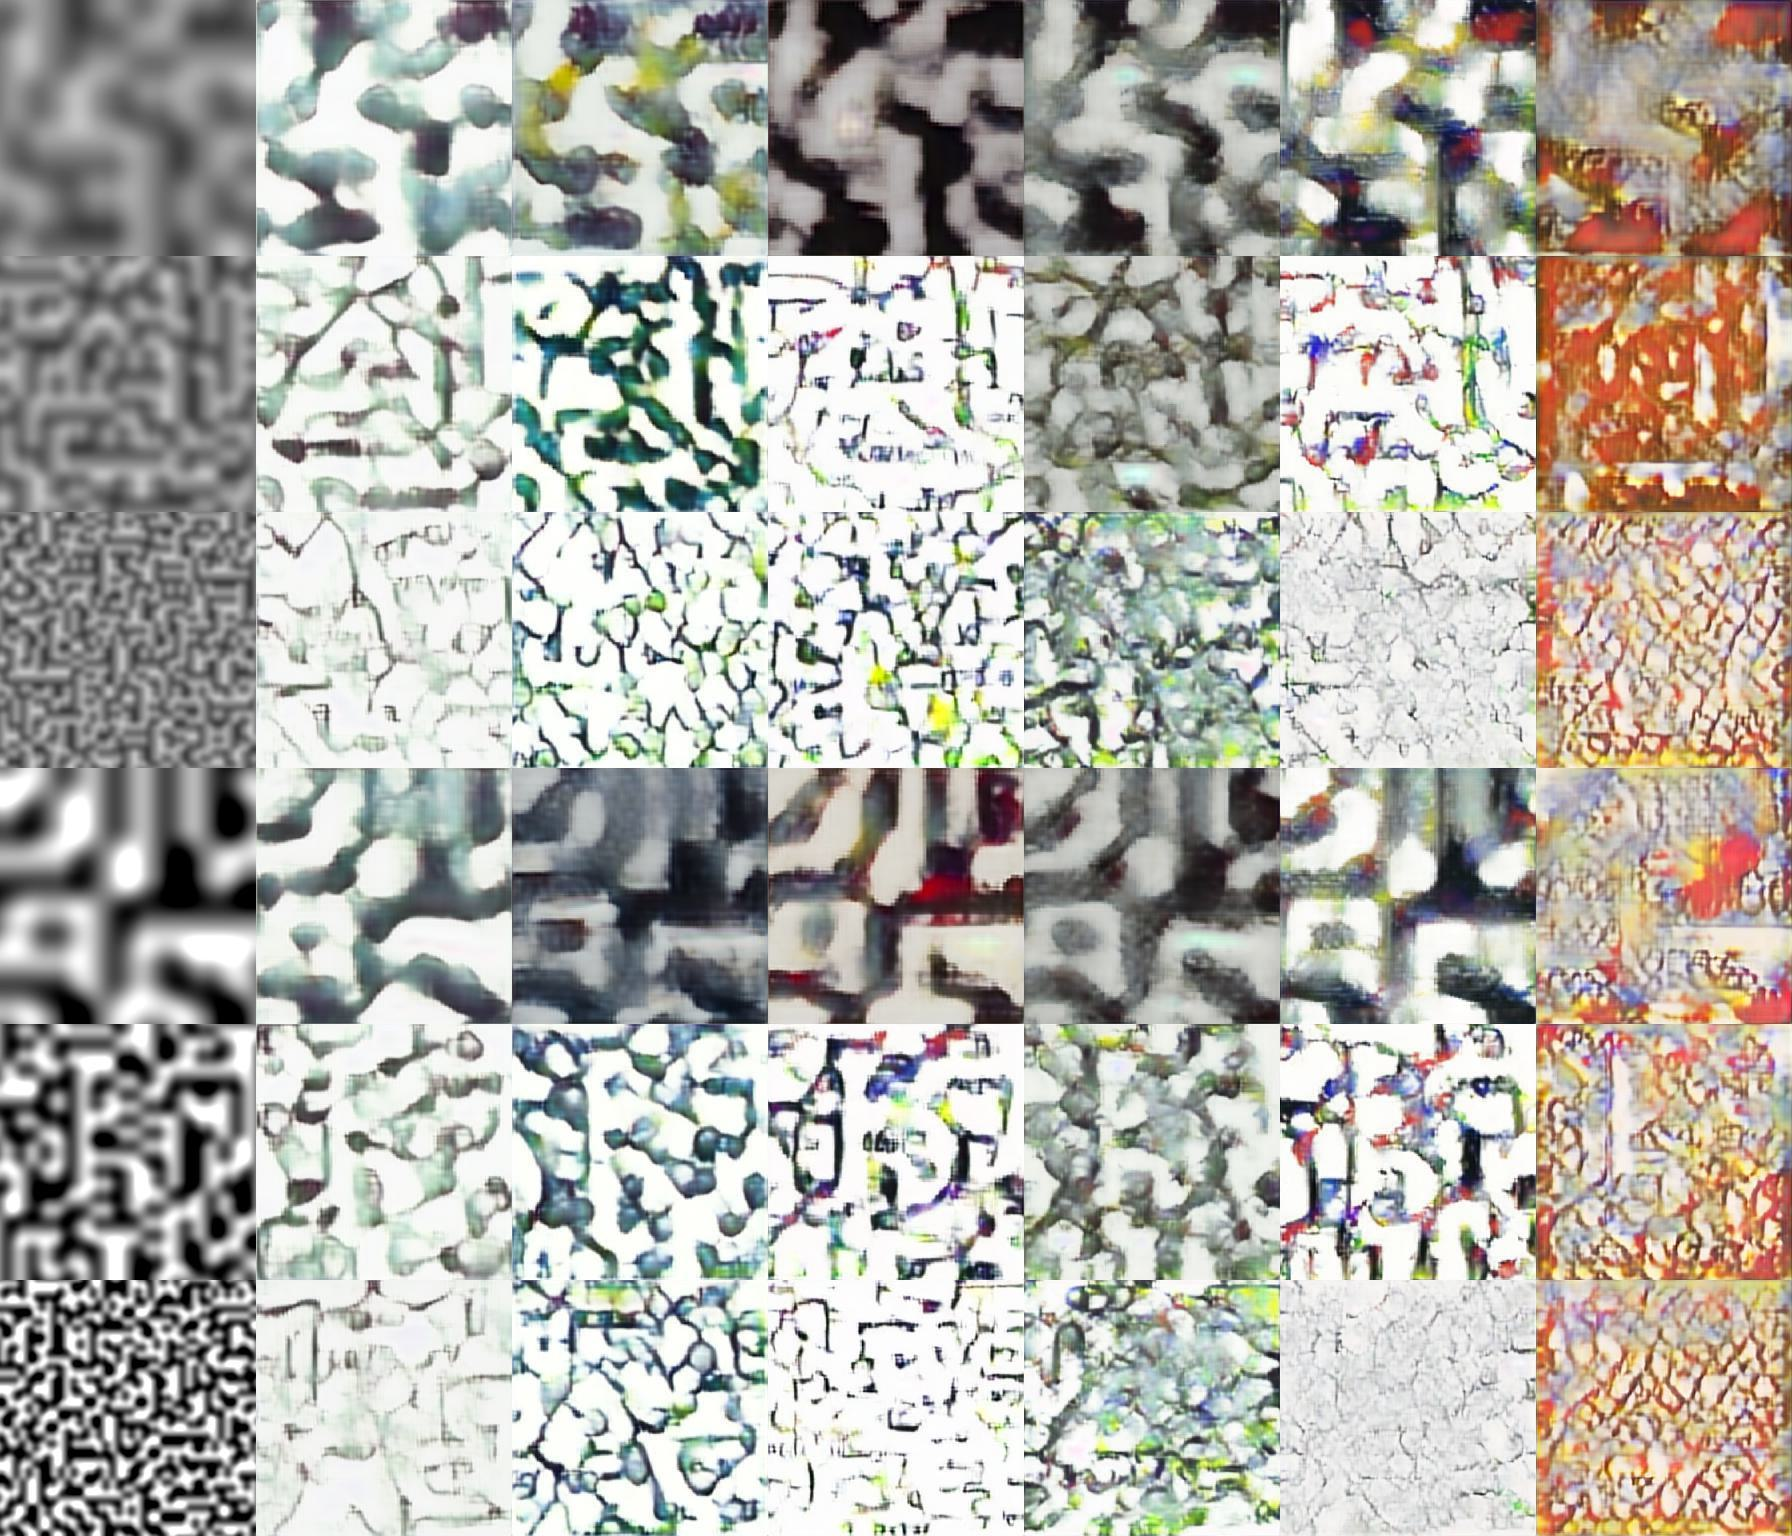
\includegraphics[scale=0.2]{imagenes/image_generation/negative256/negative256.jpg}}
    \label{fig:extraepochs}
\end{figure}

Esto puede deberse a la alta diversidad que presentan los ejemplos negativos del \textit{dataset}. Esta diversidad hace que el modelo generativo no pueda aprender, ya que las imágenes no tienen apenas características en común.

Por tanto, existen dos datasets finales con los que se entrenará cada una de las versiones del clasificador (Ver Figura \ref{fig:two_final_datasets}).
\begin{figure}[H]
\centering
    \fbox{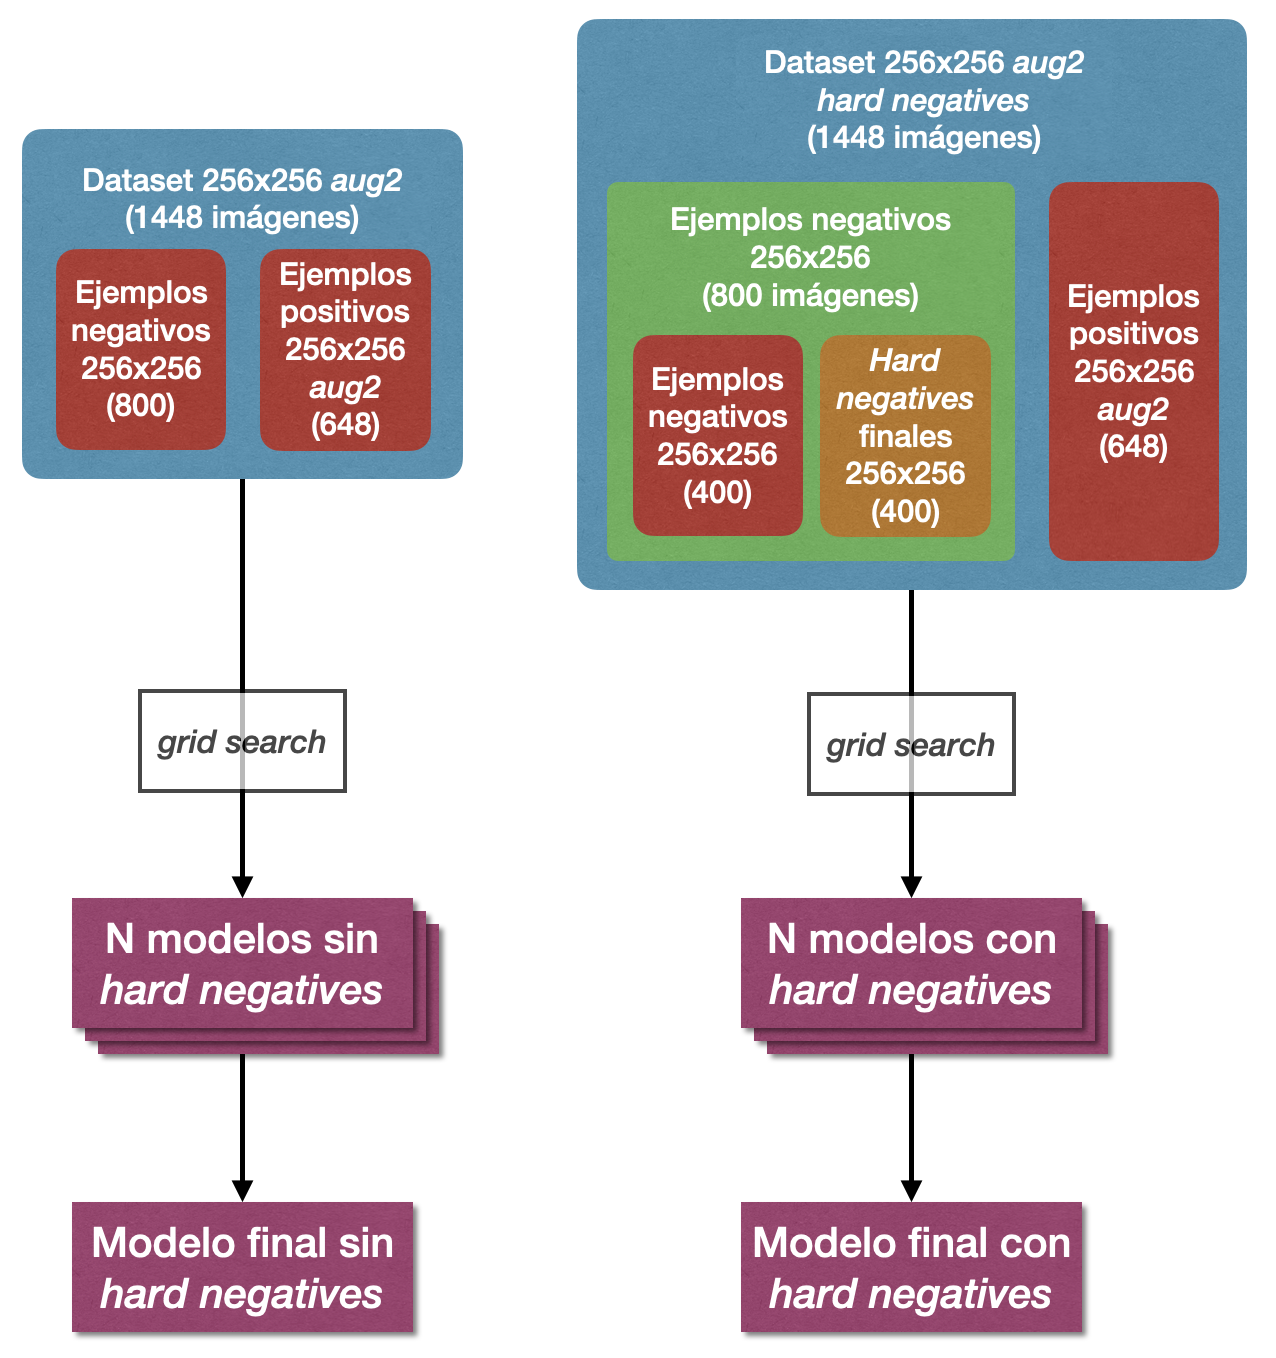
\includegraphics[scale=0.42]{imagenes/metodologia/two_datasets_aug2.png}}  
    \caption{Dos \textit{datasets} para entrenar dos clasificadores.} 
    \label{fig:two_final_datasets}
\end{figure}

\newpage
\section{Clasificación de imágenes}

Con los dos \textit{datasets} preparados \ref{fig:two_final_datasets}, paso a construir los clasificadores. Como se mencionó en el capítulo anterior, llevaré a cabo una \textit{grid search} para comprobar que arquitecturas e hiperparámetros funcionan mejor.

El código en el que se realizan los experimentos con el clasificador se encuentra en los siguientes archivos:

\vspace{0.2cm}
\dirtree{%
    .1 experiments/\DTcomment{implementación del TFG}.
    .2 image\_classifier/\DTcomment{clasificador de imágenes}.
    .3 datasets.py.
    .3 models.py.
    .3 grid\_search.py.
    .3 train\_final\_models.py.
    .3 functions.py.
}

\noindent \textit{datasets.py} declara la clase CompoundDataset, una clase que hereda la clase Dataset de Pytorch. Este objeto facilita la carga de las imágenes y su uso por las funciones y sentencias incluidas en PyTorch.

\noindent \textit{models.py} implementa cada una de las arquitecturas con las que voy a trabajar (LeNet5, AlexNet y VGG16). Se declaran cada una de sus capas, funciones de activación y el orden en el que la información fluye por estas.

\noindent \textit{grid\_search.py} implementa la \textit{grid\_search}, mediante un parámetro podemos indicar si queremos realizarla entrenando los modelos sobre el \textit{dataset} con \textit{hard negatives} o sin ellos.

\noindent \textit{train\_final\_models.py} entrena los modelos finales con la configuración decidida tras realizar la \textit{grid\_search.py}.

\noindent \textit{functions.py} declara funciones utilizadas por todos estos ficheros.

\newpage
\subsection{Clasificador sobre el \textit{dataset} sin \textit{hard negatives}}
Tras ejecutar la \textit{grid search}, se obtienen los siguientes resultados:

\begin{table}[H]
    \footnotesize
    \caption{\textit{Grid search} utilizando la arquitectura LeNet5, entrenamiento sobre \textit{dataset} sin \textit{hard negatives}.}
    \label{table:lenet-sin-hard}
\begin{tabular}{cl|llllll|}
\cline{3-8}
\multicolumn{2}{c|}{\multirow{2}{*}{}} &
    \multicolumn{6}{c|}{Optimizadores} \\ \cline{3-8} 
\multicolumn{2}{c|}{} &
    \multicolumn{2}{c|}{SGD} &
    \multicolumn{2}{c|}{Adam} &
    \multicolumn{2}{c|}{Adadelta} \\ \hline
\multicolumn{1}{|c|}{\begin{tabular}[c]{@{}c@{}}Ini. de \\ pesos\end{tabular}} &
    \multicolumn{1}{c|}{\begin{tabular}[c]{@{}c@{}}Tasa de \\ aprendizaje\end{tabular}} &
    \multicolumn{1}{c}{\begin{tabular}[c]{@{}c@{}}Error\\ medio\\ (\%)\end{tabular}} &
    \multicolumn{1}{c|}{\begin{tabular}[c]{@{}c@{}}Desv.\\ típica\\ (\%)\end{tabular}} &
    \multicolumn{1}{c}{\begin{tabular}[c]{@{}c@{}}Error\\ medio\\ (\%)\end{tabular}} &
    \multicolumn{1}{c|}{\begin{tabular}[c]{@{}c@{}}Desv.\\ típica\\ (\%)\end{tabular}} &
    \multicolumn{1}{c}{\begin{tabular}[c]{@{}c@{}}Error\\ medio\\ (\%)\end{tabular}} &
    \multicolumn{1}{c|}{\begin{tabular}[c]{@{}c@{}}Desv.\\ típica\\ (\%)\end{tabular}} \\ \hline
\multicolumn{1}{|c|}{\multirow{7}{*}{He}} &
    0.5 &
    44.715 &
    \multicolumn{1}{l|}{1.971} &
    49.593 &
    \multicolumn{1}{l|}{6.630} &
    44.715 &
    3.042 \\
\multicolumn{1}{|c|}{} &
    0.05 &
    48.130 &
    \multicolumn{1}{l|}{6.308} &
    44.715 &
    \multicolumn{1}{l|}{3.042} &
    44.715 &
    3.042 \\
\multicolumn{1}{|c|}{} &
    0.005 &
    44.715 &
    \multicolumn{1}{l|}{3.042} &
    44.715 &
    \multicolumn{1}{l|}{3.042} &
    44.715 &
    3.042 \\
\multicolumn{1}{|c|}{} &
    0.0005 &
    44.715 &
    \multicolumn{1}{l|}{3.042} &
    44.715 &
    \multicolumn{1}{l|}{3.042} &
    44.715 &
    3.042 \\
\multicolumn{1}{|c|}{} &
    0.00005 &
    44.715 &
    \multicolumn{1}{l|}{3.042} &
    44.715 &
    \multicolumn{1}{r|}{3.042} &
    48.130 &
    6.308 \\
\multicolumn{1}{|c|}{} &
    0.000005 &
    48.130 &
    \multicolumn{1}{l|}{6.308} &
    44.715 &
    \multicolumn{1}{r|}{3.042} &
    48.130 &
    6.308 \\
\multicolumn{1}{|c|}{} &
    0.0000005 &
    48.130 &
    \multicolumn{1}{l|}{6.308} &
    48.130 &
    \multicolumn{1}{r|}{6.308} &
    48.130 &
    6.308 \\ \hline
\multicolumn{1}{|c|}{\multirow{7}{*}{Xavier}} &
    0.5 &
    48.130 &
    \multicolumn{1}{l|}{6.308} &
    48.943 &
    \multicolumn{1}{l|}{6.540} &
    26.260 &
    \multicolumn{1}{r|}{16.213} \\
\multicolumn{1}{|c|}{} &
    0.05 &
    27.967 &
    \multicolumn{1}{l|}{14.734} &
    44.715 &
    \multicolumn{1}{l|}{3.042} &
    33.252 &
    11.226 \\
\multicolumn{1}{|c|}{} &
    0.005 &
    43.902 &
    \multicolumn{1}{l|}{4.378} &
    44.715 &
    \multicolumn{1}{l|}{3.042} &
    43.740 &
    4.685 \\
\multicolumn{1}{|c|}{} &
    0.0005 &
    44.715 &
    \multicolumn{1}{l|}{3.042} &
    44.715 &
    \multicolumn{1}{r|}{3.042} &
    44.715 &
    3.042 \\
\multicolumn{1}{|c|}{} &
    0.00005 &
    44.715 &
    \multicolumn{1}{l|}{3.042} &
    41.951 &
    \multicolumn{1}{r|}{6.018} &
    48.130 &
    6.308 \\
\multicolumn{1}{|c|}{} &
    0.000005 &
    48.130 &
    \multicolumn{1}{l|}{6.308} &
    40.813 &
    \multicolumn{1}{l|}{6.596} &
    48.130 &
    6.308 \\
\multicolumn{1}{|c|}{} &
    0.0000005 &
    48.130 &
    \multicolumn{1}{l|}{6.308} &
    44.715 &
    \multicolumn{1}{l|}{3.042} &
    48.130 &
    6.308 \\ \hline
\end{tabular}
\label{table:lenetsinhard}
\end{table}


% Please add the following required packages to your document preamble:
% \usepackage{multirow}
\begin{table}[H]
    \footnotesize
    \caption{\textit{Grid search} utilizando la arquitectura AlexNet, entrenamiento sobre \textit{dataset} sin \textit{hard negatives}.}
    \label{table:alexnet-sin-hard}
\begin{tabular}{cl|llllll|}
\cline{3-8}
\multicolumn{2}{c|}{\multirow{2}{*}{}} &
    \multicolumn{6}{c|}{Optimizadores} \\ \cline{3-8} 
\multicolumn{2}{c|}{} &
    \multicolumn{2}{c|}{SGD} &
    \multicolumn{2}{c|}{Adam} &
    \multicolumn{2}{c|}{Adadelta} \\ \hline
\multicolumn{1}{|c|}{\begin{tabular}[c]{@{}c@{}}Ini. de \\ pesos\end{tabular}} &
    \multicolumn{1}{c|}{\begin{tabular}[c]{@{}c@{}}Tasa de \\ aprendizaje\end{tabular}} &
    \multicolumn{1}{c}{\begin{tabular}[c]{@{}c@{}}Error\\ medio\\ (\%)\end{tabular}} &
    \multicolumn{1}{c|}{\begin{tabular}[c]{@{}c@{}}Desv.\\ típica\\ (\%)\end{tabular}} &
    \multicolumn{1}{c}{\begin{tabular}[c]{@{}c@{}}Error\\ medio\\ (\%)\end{tabular}} &
    \multicolumn{1}{c|}{\begin{tabular}[c]{@{}c@{}}Desv.\\ típica\\ (\%)\end{tabular}} &
    \multicolumn{1}{c}{\begin{tabular}[c]{@{}c@{}}Error\\ medio\\ (\%)\end{tabular}} &
    \multicolumn{1}{c|}{\begin{tabular}[c]{@{}c@{}}Desv.\\ típica\\ (\%)\end{tabular}} \\ \hline
\multicolumn{1}{|c|}{\multirow{7}{*}{He}} &
    0.5 &
    44.715 &
    \multicolumn{1}{l|}{3.042} &
    49.268 &
    \multicolumn{1}{l|}{7.061} &
    5.041 &
    1.691 \\
\multicolumn{1}{|c|}{} &
    0.05 &
    5.528 &
    \multicolumn{1}{l|}{1.809} &
    53.008 &
    \multicolumn{1}{l|}{5.732} &
    3.984 &
    2.061 \\
\multicolumn{1}{|c|}{} &
    0.005 &
    3.984 &
    \multicolumn{1}{l|}{1.091} &
    42.683 &
    \multicolumn{1}{l|}{6.814} &
    5.366 &
    1.449 \\
\multicolumn{1}{|c|}{} &
    0.0005 &
    44.634 &
    \multicolumn{1}{l|}{2.937} &
    3.740 &
    \multicolumn{1}{l|}{1.128} &
    44.715 &
    3.042 \\
\multicolumn{1}{|c|}{} &
    0.00005 &
    44.715 &
    \multicolumn{1}{l|}{3.042} &
    3.821 &
    \multicolumn{1}{r|}{0.843} &
    45.691 &
    2.104 \\
\multicolumn{1}{|c|}{} &
    0.000005 &
    48.618 &
    \multicolumn{1}{l|}{5.782} &
    4.309 &
    \multicolumn{1}{r|}{1.786} &
    48.699 &
    6.601 \\
\multicolumn{1}{|c|}{} &
    0.0000005 &
    49.675 &
    \multicolumn{1}{l|}{7.409} &
    5.772 &
    \multicolumn{1}{r|}{1.298} &
    50.000 &
    7.479 \\ \hline
\multicolumn{1}{|c|}{\multirow{7}{*}{Xavier}} &
    0.5 &
    44.715 &
    \multicolumn{1}{l|}{3.042} &
    46.992 &
    \multicolumn{1}{l|}{7.281} &
    4.472 &
    \multicolumn{1}{r|}{0.909} \\
\multicolumn{1}{|c|}{} &
    0.05 &
    5.691 &
    \multicolumn{1}{l|}{1.437} &
    45.854 &
    \multicolumn{1}{l|}{7.113} &
    3.984 &
    1.661 \\
\multicolumn{1}{|c|}{} &
    0.005 &
    4.390 &
    \multicolumn{1}{l|}{1.937} &
    44.634 &
    \multicolumn{1}{l|}{3.154} &
    4.065 &
    2.370 \\
\multicolumn{1}{|c|}{} &
    0.0005 &
    5.610 &
    \multicolumn{1}{l|}{2.360} &
    4.146 &
    \multicolumn{1}{r|}{0.782} &
    5.772 &
    1.505 \\
\multicolumn{1}{|c|}{} &
    0.00005 &
    31.789 &
    \multicolumn{1}{l|}{2.325} &
    3.333 &
    \multicolumn{1}{r|}{1.532} &
    34.228 &
    2.625 \\
\multicolumn{1}{|c|}{} &
    0.000005 &
    44.959 &
    \multicolumn{1}{l|}{2.751} &
    4.228 &
    \multicolumn{1}{l|}{2.548} &
    45.041 &
    2.687 \\
\multicolumn{1}{|c|}{} &
    0.0000005 &
    46.748 &
    \multicolumn{1}{l|}{7.157} &
    5.122 &
    \multicolumn{1}{l|}{1.537} &
    47.805 &
    6.275 \\ \hline
\end{tabular}
\label{table:alexnetsinhard}
\end{table}


% Please add the following required packages to your document preamble:
% \usepackage{multirow}
\begin{table}[H]
    \footnotesize
    \caption{\textit{Grid search} utilizando la arquitectura VGG16, entrenamiento sobre \textit{dataset} sin \textit{hard negatives}.}
    \label{table:vgg16-sin-hard}
\begin{tabular}{cl|llllll|}
\cline{3-8}
\multicolumn{2}{c|}{\multirow{2}{*}{}} &
    \multicolumn{6}{c|}{Optimizadores} \\ \cline{3-8} 
\multicolumn{2}{c|}{} &
    \multicolumn{2}{c|}{SGD} &
    \multicolumn{2}{c|}{Adam} &
    \multicolumn{2}{c|}{Adadelta} \\ \hline
\multicolumn{1}{|c|}{\begin{tabular}[c]{@{}c@{}}Ini. de \\ pesos\end{tabular}} &
    \multicolumn{1}{c|}{\begin{tabular}[c]{@{}c@{}}Tasa de \\ aprendizaje\end{tabular}} &
    \multicolumn{1}{c}{\begin{tabular}[c]{@{}c@{}}Error\\ medio\\ (\%)\end{tabular}} &
    \multicolumn{1}{c|}{\begin{tabular}[c]{@{}c@{}}Desv.\\ típica\\ (\%)\end{tabular}} &
    \multicolumn{1}{c}{\begin{tabular}[c]{@{}c@{}}Error\\ medio\\ (\%)\end{tabular}} &
    \multicolumn{1}{c|}{\begin{tabular}[c]{@{}c@{}}Desv.\\ típica\\ (\%)\end{tabular}} &
    \multicolumn{1}{c}{\begin{tabular}[c]{@{}c@{}}Error\\ medio\\ (\%)\end{tabular}} &
    \multicolumn{1}{c|}{\begin{tabular}[c]{@{}c@{}}Desv.\\ típica\\ (\%)\end{tabular}} \\ \hline
\multicolumn{1}{|c|}{\multirow{7}{*}{He}} &
    0.5 &
    44.715 &
    \multicolumn{1}{l|}{3.042} &
    52.439 &
    \multicolumn{1}{l|}{5.126} &
    44.715 &
    3.042 \\
\multicolumn{1}{|c|}{} &
    0.05 &
    44.715 &
    \multicolumn{1}{l|}{3.042} &
    44.797 &
    \multicolumn{1}{l|}{3.101} &
    44.715 &
    3.042 \\
\multicolumn{1}{|c|}{} &
    0.005 &
    44.715 &
    \multicolumn{1}{l|}{3.042} &
    44.715 &
    \multicolumn{1}{l|}{3.042} &
    44.715 &
    3.042 \\
\multicolumn{1}{|c|}{} &
    0.0005 &
    44.715 &
    \multicolumn{1}{l|}{3.042} &
    44.715 &
    \multicolumn{1}{l|}{3.042} &
    48.537 &
    7.062 \\
\multicolumn{1}{|c|}{} &
    0.00005 &
    48.618 &
    \multicolumn{1}{l|}{6.938} &
    3.577 &
    \multicolumn{1}{r|}{0.668} &
    50.569 &
    5.436 \\
\multicolumn{1}{|c|}{} &
    0.000005 &
    50.650 &
    \multicolumn{1}{l|}{5.451} &
    5.772 &
    \multicolumn{1}{r|}{2.020} &
    50.813 &
    5.806 \\
\multicolumn{1}{|c|}{} &
    0.0000005 &
    50.813 &
    \multicolumn{1}{l|}{5.806} &
    22.764 &
    \multicolumn{1}{r|}{7.643} &
    50.732 &
    5.766 \\ \hline
\multicolumn{1}{|c|}{\multirow{7}{*}{Xavier}} &
    0.5 &
    44.715 &
    \multicolumn{1}{l|}{3.042} &
    49.350 &
    \multicolumn{1}{l|}{6.463} &
    44.715 &
    \multicolumn{1}{r|}{3.042} \\
\multicolumn{1}{|c|}{} &
    0.05 &
    7.398 &
    \multicolumn{1}{l|}{1.872} &
    44.715 &
    \multicolumn{1}{l|}{3.042} &
    3.577 &
    1.849 \\
\multicolumn{1}{|c|}{} &
    0.005 &
    5.041 &
    \multicolumn{1}{l|}{2.065} &
    44.715 &
    \multicolumn{1}{l|}{3.042} &
    7.317 &
    1.285 \\
\multicolumn{1}{|c|}{} &
    0.0005 &
    44.309 &
    \multicolumn{1}{l|}{3.613} &
    44.715 &
    \multicolumn{1}{r|}{3.042} &
    44.390 &
    3.697 \\
\multicolumn{1}{|c|}{} &
    0.00005 &
    46.260 &
    \multicolumn{1}{l|}{2.139} &
    3.252 &
    \multicolumn{1}{r|}{1.113} &
    48.130 &
    4.010 \\
\multicolumn{1}{|c|}{} &
    0.000005 &
    49.593 &
    \multicolumn{1}{l|}{4.388} &
    4.878 &
    \multicolumn{1}{l|}{2.802} &
    49.837 &
    4.289 \\
\multicolumn{1}{|c|}{} &
    0.0000005 &
    49.919 &
    \multicolumn{1}{l|}{4.267} &
    6.667 &
    \multicolumn{1}{l|}{2.328} &
    50.163 &
    4.514 \\ \hline
\end{tabular}
\label{table:vggsinhard}
\end{table}

Es curioso observar que, mientras en AlexNet \ref{table:alexnetsinhard} y VGG16 \ref{table:vggsinhard} se reduce el error a menos del 5\% con ciertas combinaciones de hiperparámetros, en LeNet5 \ref{table:lenetsinhard} no ocurre esto. En concreto, uno de los mejores resultados que obtiene esta arquitectura es un 27.96\% de error con una desviación media del 14.73\% entre las 5 iteraciones de la validación cruzada. Tras revisar la implementación, no creo que exista ningún error. ¿A qué puede deberse? ¿Puede ser que el modelo, por su pequeño tamaño, no tenga la capacidad suficiente para aprender este tipo de imágenes?

\begin{figure}[H]
\centering
    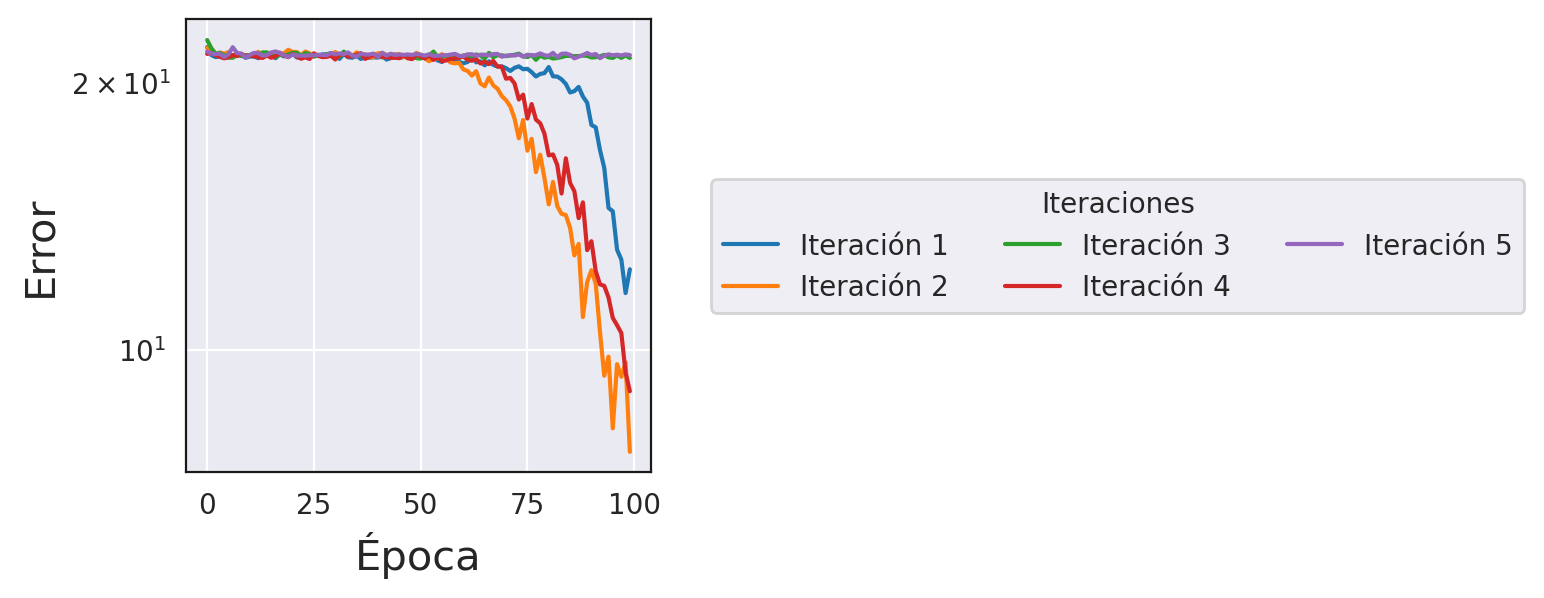
\includegraphics[scale=0.65]{imagenes/image_classification/original_dataset/loss1.png}
    \caption{Variación del error durante el entrenamiento utilizando la configuración LeNet5-Xavier-0.05-SGD. Las iteraciones se corresponden con las producidas durante la validación cruzada.}
    \label{fig:te-LeNet5-Xavier-0.05-SGD}
\end{figure}

La Figura \ref{fig:te-LeNet5-Xavier-0.05-SGD} muestra la disminución del error durante el entrenamiento del modelo con la configuración de la que hablo en el párrafo anterior. Se puede observar como decrece solo en 3 de las 5 iteraciones. Seguramente esta sea la causa de que exista una alta desviación de error entre iteraciones (14.73\%), ya que en algunas el algoritmo tiende a converger pero en otras no.

En la Figura \ref{te-lenet} se puede comprobar como en la mayoría de configuraciones el error o bien no decrece o bien existe una gran diferencia en el valor que toma entre iteraciones.

\begin{figure}[H]
\centering
    \begin{subfigure}{.47\textwidth}
        \centering
        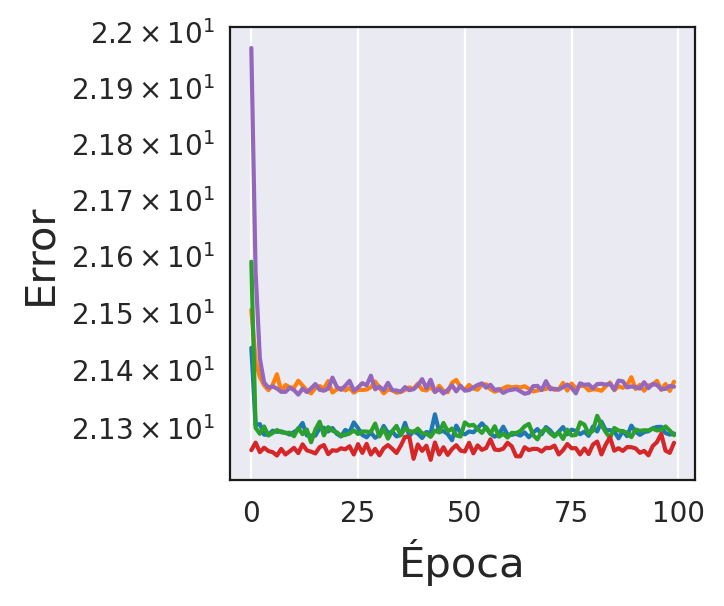
\includegraphics[width=1\linewidth]{imagenes/image_classification/original_dataset/loss2.png}
        \caption{LeNet5 - He - Adam - 0.00005}
    \end{subfigure}%
    \begin{subfigure}{.47\textwidth}
        \centering
        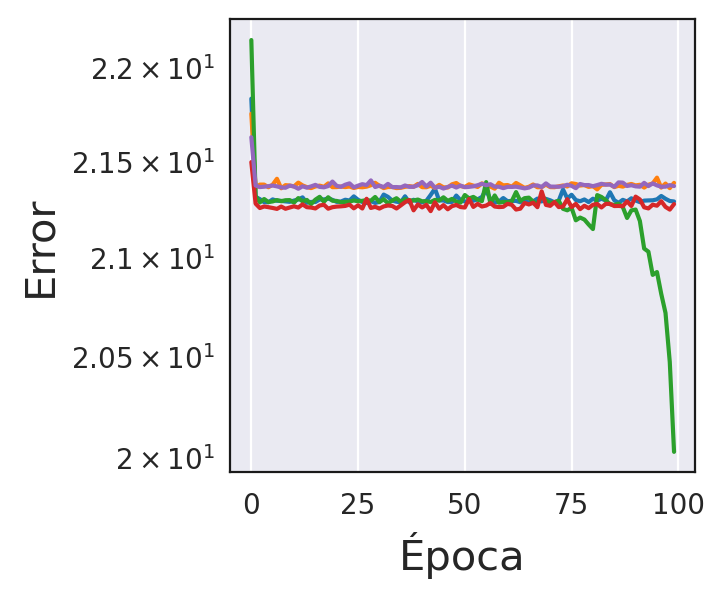
\includegraphics[width=1\linewidth]{imagenes/image_classification/original_dataset/loss3.png}
        \caption{LeNet5 - Xavier - Adam - 0.00005}
    \end{subfigure}%

    \bigskip

    \begin{subfigure}{.47\textwidth}
        \centering
        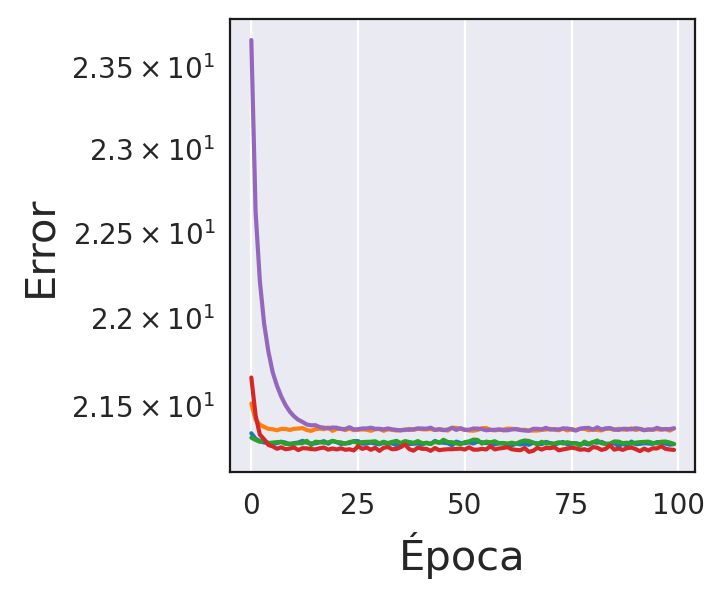
\includegraphics[width=1\linewidth]{imagenes/image_classification/original_dataset/loss4.png}
        \caption{LeNet5 - He - AdaDelta - 0.005}
    \end{subfigure}%
    \begin{subfigure}{.47\textwidth}
        \centering
        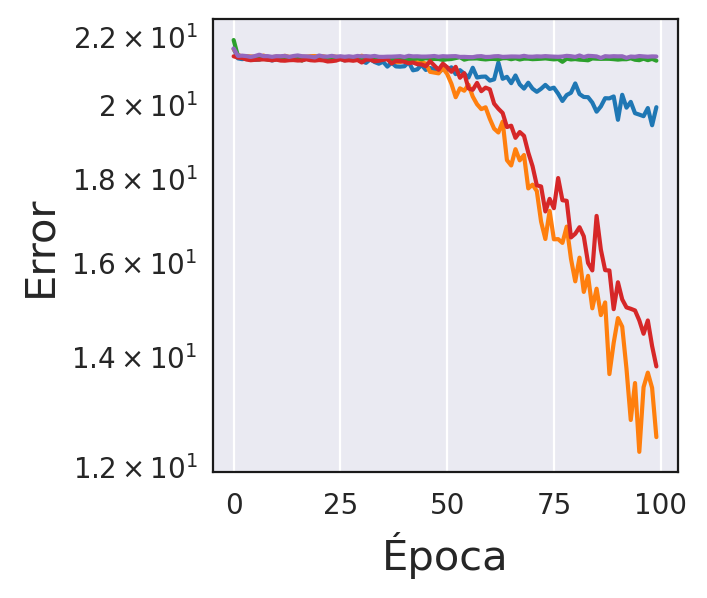
\includegraphics[width=1\linewidth]{imagenes/image_classification/original_dataset/loss5.png}
        \caption{LeNet5 - Xavier - AdaDelta - 0.05}
    \end{subfigure}

    \caption{Más ejemplos de cómo varía el error durante el entrenamiento utilizando diferentes configuraciones sobre LeNet5.}
    \label{te-lenet}
\end{figure}

Es probable que la arquitectura LeNet5 no tenga capacidad para modelar el problema debido a su pequeño tamaño. Vamos a realizar otro experimento, entrenar un modelo LeNet5 con un \textit{dataset} reducido para ver si el error de entrenamiento decrece con mayor facilidad. Este será una muestra aleatoria del original.

\begin{figure}[H]
\centering
    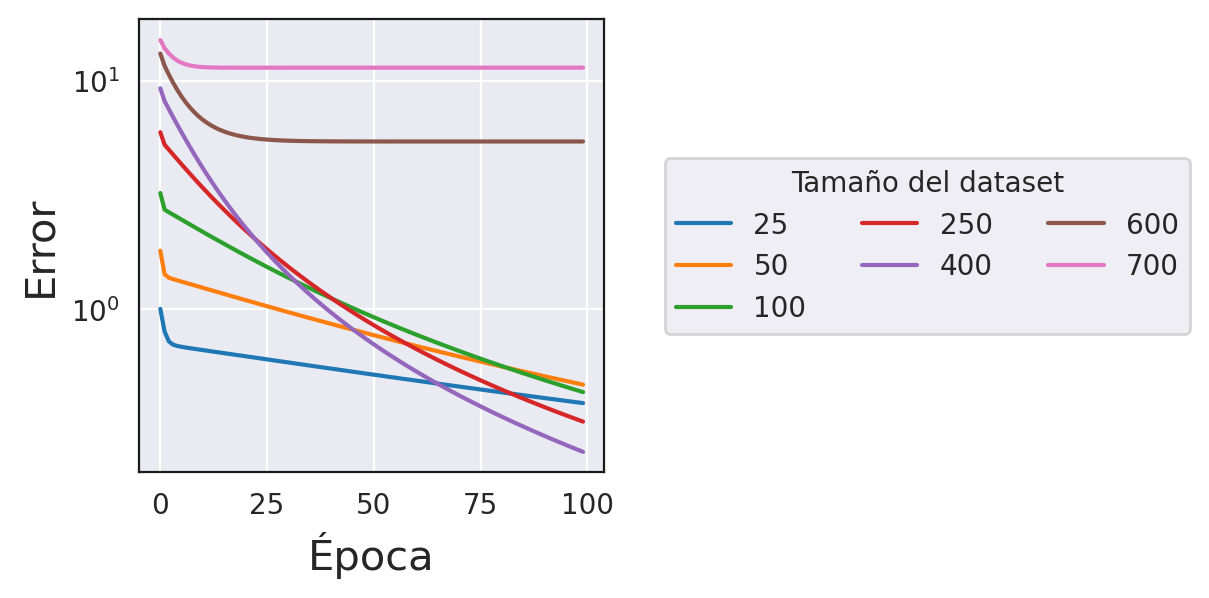
\includegraphics[scale=0.64]{imagenes/image_classification/original_dataset/loss_smalldataset.png}
    \caption{Modelos entrenados con la configuración LeNet5-He-Adam-0.00005, utilizando \textit{datasets} de diferente tamaño (desde 25 hasta 700 imágenes).}
    \label{fig:loss-smalldataset}
\end{figure}

En la Figura \ref{fig:loss-smalldataset} se observa como utilizando conjuntos de datos de entrenamiento de menor tamaño se consigue que el error decrezca con mayor facilidad. Hasta un \textit{dataset} de tamaño 400, el error reduce de forma continua durante todo el entrenamiento, pero a partir de 600 el error se estanca. Introducir un mayor número de imágenes de entrenamiento genera mayor diversidad, que tiene que ser capturada por el modelo. Si el modelo es demasiado pequeño no será capaz de capturarla y por tanto el error no se reducirá mientras se entrena.

Por ello AlexNet y VGG16 serán las arquitecturas que se tengan en cuenta a la hora de elegir la configuración del modelo final. Entre ellas, el mejor resultado viene dado por VGG16, con la configuración VGG16-Xavier-Adam-0.00005. Se obtiene un error del 3.252\%, con una desviación entre iteraciones de la validación cruzada del 1.113\%. Vamos a graficar el error de entrenamiento en cada iteración en la Figura \ref{fig:loss_vgg16_xavier_adam_00005}

\begin{figure}[H]
\centering
    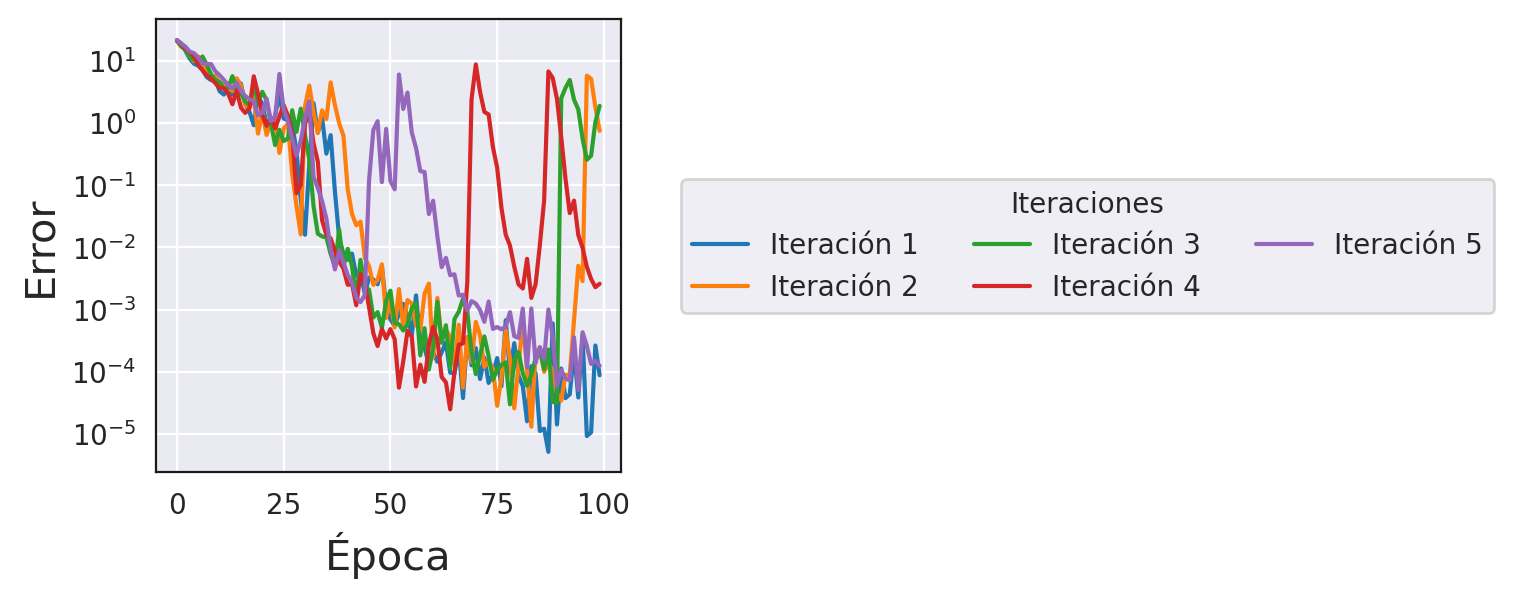
\includegraphics[scale=0.6]{imagenes/image_classification/original_dataset/loss_vgg16_xavier_adam_00005.png}
    \caption{Evolución del error de \textit{training} durante el entrenamiento de un modelo con configuración VGG16-Xavier-Adam-0.00005 sobre un \textit{dataset} sin \textit{hard negatives}.}
    \label{fig:loss_vgg16_xavier_adam_00005}
\end{figure}

Se observan muchos picos, en algunos casos ascendiendo al valor de error inicial. Esto puede deberse a diversos factores, como son la explosión del gradiente (producida por el valor que toma la tasa de aprendizaje o por su inadecuada actualización en el algoritmo de optimización) o el un tamaño de minilote demasiado pequeño y que sea culpable de que el gradiente oscile. ¿Qué ocurre en otras configuraciones que también devuelven porcentajes de error razonables en las tablas \ref{table:alexnet-sin-hard} y \ref{table:vgg16-sin-hard}?

\begin{figure}[H]
\centering
    \begin{subfigure}{.45\textwidth}
        \centering
        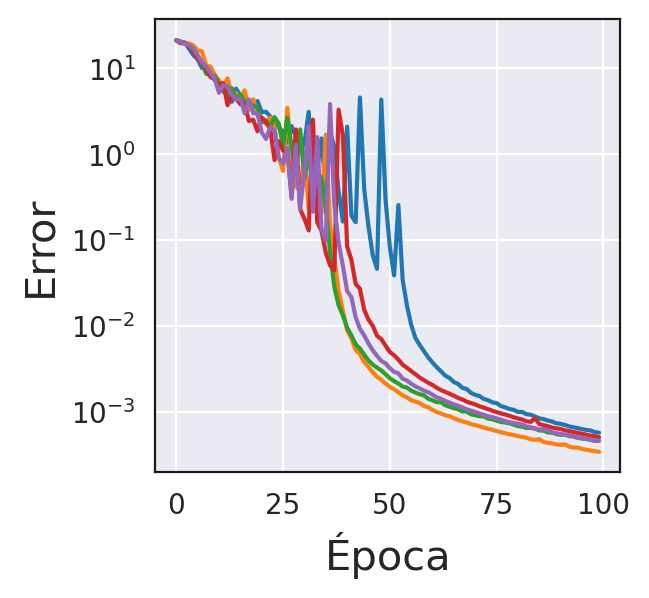
\includegraphics[width=1\linewidth]{imagenes/image_classification/original_dataset/loss_alexnet_he_adadelta_05.png}
        \caption{AlexNet-He-Adadelta-0.05 \hspace{\textwidth} Error medio (\%): 3.984 \hspace{\textwidth} Desv. típica (\%): 2.061}
    \end{subfigure}%
    \begin{subfigure}{.45\textwidth}
        \centering
        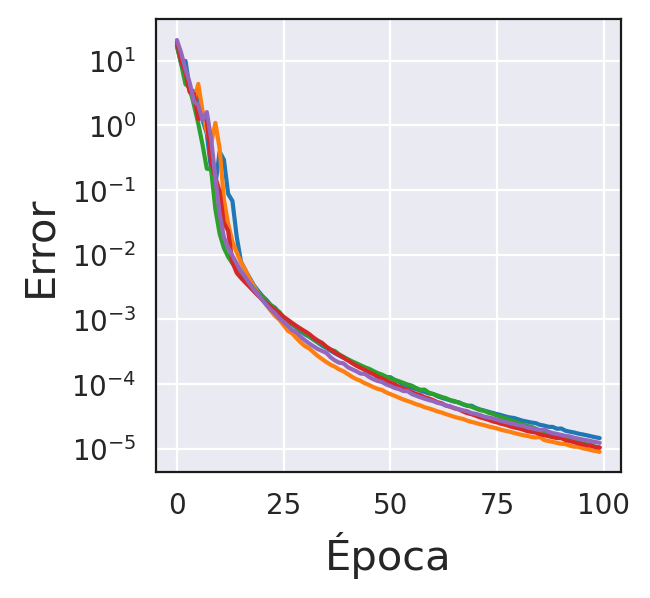
\includegraphics[width=1\linewidth]{imagenes/image_classification/original_dataset/loss_alexnet_xavier_adam_00005.png}
        \caption{AlexNet-Xavier-Adam-0.00005 \hspace{\textwidth} Error medio (\%): 3.333 \hspace{\textwidth} Desv. típica (\%): 1.532}
    \end{subfigure}%

    \bigskip

    \begin{subfigure}{.45\textwidth}
        \centering
        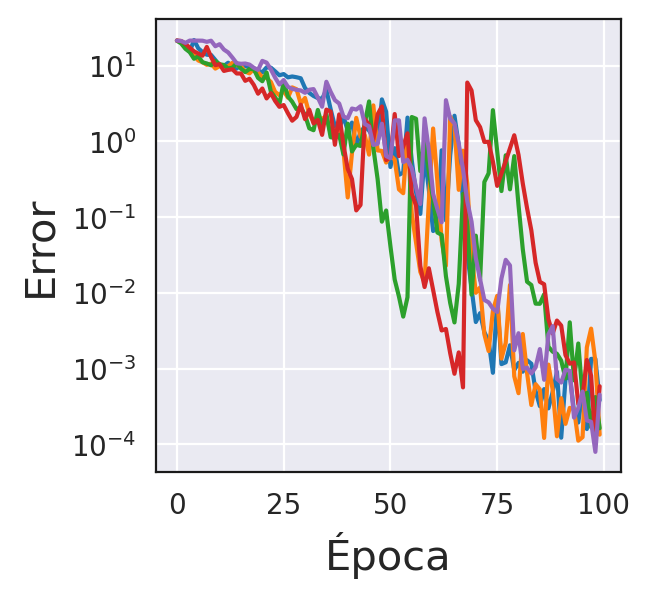
\includegraphics[width=1\linewidth]{imagenes/image_classification/original_dataset/loss_vgg16_he_adam_00005.png}
        \caption{VGG16-He-Adam-0.00005 \hspace{\textwidth} Error medio (\%): 3.577 \hspace{\textwidth} Desv. típica (\%): 0.668}
    \end{subfigure}%
    \begin{subfigure}{.45\textwidth}
        \centering
        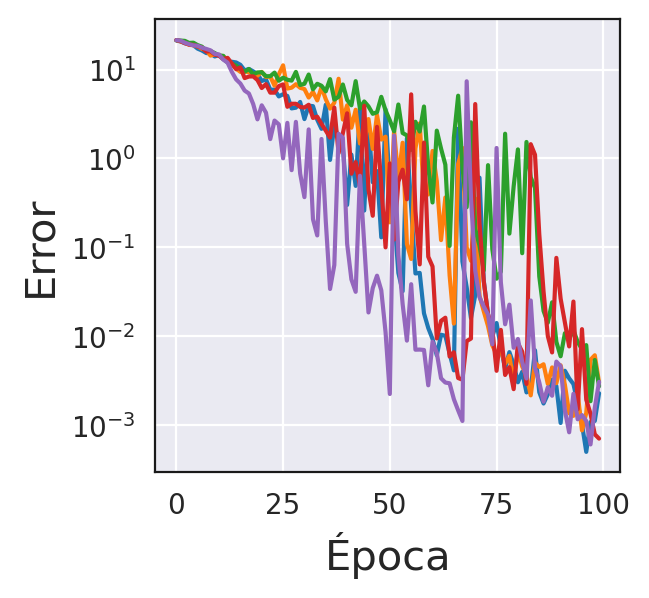
\includegraphics[width=1\linewidth]{imagenes/image_classification/original_dataset/loss_vgg16_xavier_adadelta_05.png}
        \caption{VGG16-Xavier-AdaDelta-0.05 \hspace{\textwidth} Error medio (\%): 3.577 \hspace{\textwidth} Desv. típica (\%): 1.849}
    \end{subfigure}

    \caption{Más ejemplos de cómo varía el error durante el entrenamiento de diferentes modelos utilizando configuraciones basadas en LeNet5, sobre un \textit{dataset} sin \textit{hard negatives}.}
\end{figure}

Se observa como en los modelos basados en VGG16 existe una mayor oscilación del error. Se podría probar a utilizar un tamaño de minilote mayor (64, 128 o 256). Por otro lado, en los basados en AlexNet se observa una curva más suave. Por ello, ya que la diferencia de error es mínima entre todos estos modelos, se va a utilizar como configuración para entrenar el modelo final AlexNet-Xavier-Adam-0.00005, cuya curva de error es muy suave.

El modelo final se entrenará sobre la partición \textit{train} (de 1230 elementos, 85\% del dataset) y se dará una evaluación final sobre la \textit{test} (de 218 elementos, 15\% del dataset), tal y como se representa en la figura \ref{fig:train-test}.

\begin{table}[H]
    \footnotesize
    \centering
    \caption{Porcentaje de error del modelo final sin \textit{hard negatives}.}
\begin{tabular}{@{}ll@{}}
\toprule
Modelo final              & \multicolumn{1}{c}{\begin{tabular}[c]{@{}c@{}}Error sobre la\\ partición de \textit{test}\end{tabular}} \\ \midrule
AlexNet-Xavier-Adam-0.00005 & 2.752\%                                                                                        \\ \bottomrule
\end{tabular}
\end{table}

Se mostró este resultado a los científicos israelíes y quedaron conformes. Durante el entrenamiento el error decreció como se puede observar en la Figura \ref{fig:original-loss-final-model}.

\begin{figure}[H]
\centering
    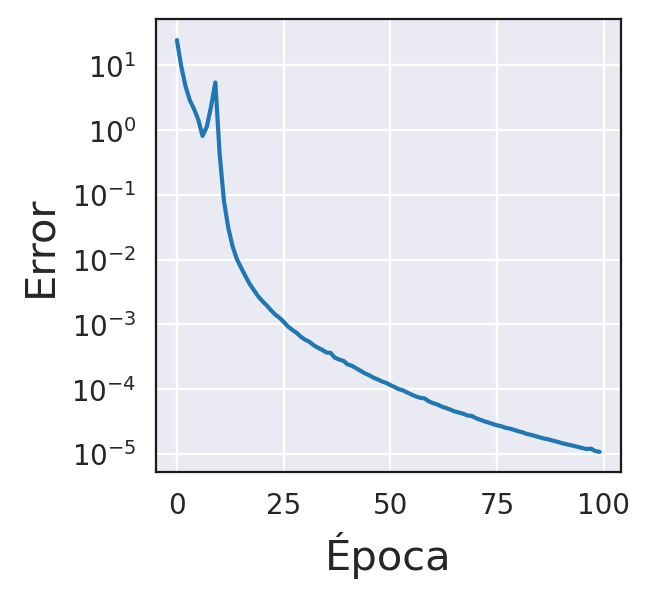
\includegraphics[scale=0.67]{imagenes/image_classification/original_dataset/loss_final_model.png}
    \caption{Evolución del error de \textit{training} durante el entrenamiento del modelo final sobre el \textit{dataset} sin \textit{hard negatives}.}
    \label{fig:original-loss-final-model}
\end{figure}


\newpage
\subsection{Clasificador sobre el \textit{dataset} con \textit{hard negatives}}
Se realiza el mismo proceso que he seguido en la sección anterior, ahora utilizando el \textit{dataset} que contiene un 50\% de ejemplos negativos originales y un 50\% sintéticos creados a partir de los modelos generadores.

\begin{table}[H]
    \footnotesize
    \caption{\textit{Grid search} utilizando la arquitectura LeNet5, entrenamiento sobre \textit{dataset} con \textit{hard negatives}.}
\begin{tabular}{cl|llllll|}
\cline{3-8}
\multicolumn{2}{c|}{\multirow{2}{*}{}} &
    \multicolumn{6}{c|}{Optimizadores} \\ \cline{3-8} 
\multicolumn{2}{c|}{} &
    \multicolumn{2}{c|}{SGD} &
    \multicolumn{2}{c|}{Adam} &
    \multicolumn{2}{c|}{Adadelta} \\ \hline
\multicolumn{1}{|c|}{\begin{tabular}[c]{@{}c@{}}Ini. de \\ pesos\end{tabular}} &
    \multicolumn{1}{c|}{\begin{tabular}[c]{@{}c@{}}Tasa de \\ aprendizaje\end{tabular}} &
    \multicolumn{1}{c}{\begin{tabular}[c]{@{}c@{}}Error\\ medio\\ (\%)\end{tabular}} &
    \multicolumn{1}{c|}{\begin{tabular}[c]{@{}c@{}}Desv.\\ típica\\ (\%)\end{tabular}} &
    \multicolumn{1}{c}{\begin{tabular}[c]{@{}c@{}}Error\\ medio\\ (\%)\end{tabular}} &
    \multicolumn{1}{c|}{\begin{tabular}[c]{@{}c@{}}Desv.\\ típica\\ (\%)\end{tabular}} &
    \multicolumn{1}{c}{\begin{tabular}[c]{@{}c@{}}Error\\ medio\\ (\%)\end{tabular}} &
    \multicolumn{1}{c|}{\begin{tabular}[c]{@{}c@{}}Desv.\\ típica\\ (\%)\end{tabular}} \\ \hline
\multicolumn{1}{|c|}{\multirow{7}{*}{He}} &
    0.5 &
    44.715 &
    \multicolumn{1}{l|}{1.971} &
    48.943 &
    \multicolumn{1}{l|}{6.540} &
    44.715 &
    3.042 \\
\multicolumn{1}{|c|}{} &
    0.05 &
    48.130 &
    \multicolumn{1}{l|}{6.308} &
    44.715 &
    \multicolumn{1}{l|}{3.042} &
    44.715 &
    3.042 \\
\multicolumn{1}{|c|}{} &
    0.005 &
    44.715 &
    \multicolumn{1}{l|}{3.042} &
    44.715 &
    \multicolumn{1}{l|}{3.042} &
    44.715 &
    3.042 \\
\multicolumn{1}{|c|}{} &
    0.0005 &
    44.715 &
    \multicolumn{1}{l|}{3.042} &
    44.715 &
    \multicolumn{1}{l|}{3.042} &
    44.715 &
    3.042 \\
\multicolumn{1}{|c|}{} &
    0.00005 &
    44.715 &
    \multicolumn{1}{l|}{3.042} &
    44.715 &
    \multicolumn{1}{r|}{3.042} &
    48.130 &
    6.308 \\
\multicolumn{1}{|c|}{} &
    0.000005 &
    48.130 &
    \multicolumn{1}{l|}{6.308} &
    44.715 &
    \multicolumn{1}{r|}{3.042} &
    48.130 &
    6.308 \\
\multicolumn{1}{|c|}{} &
    0.0000005 &
    48.130 &
    \multicolumn{1}{l|}{6.308} &
    48.130 &
    \multicolumn{1}{r|}{6.308} &
    48.130 &
    6.308 \\ \hline
\multicolumn{1}{|c|}{\multirow{7}{*}{Xavier}} &
    0.5 &
    48.130 &
    \multicolumn{1}{l|}{6.308} &
    48.130 &
    \multicolumn{1}{l|}{6.308} &
    44.715 &
    \multicolumn{1}{r|}{3.042} \\
\multicolumn{1}{|c|}{} &
    0.05 &
    48.130 &
    \multicolumn{1}{l|}{6.308} &
    44.715 &
    \multicolumn{1}{l|}{3.042} &
    45.610 &
    2.545 \\
\multicolumn{1}{|c|}{} &
    0.005 &
    45.041 &
    \multicolumn{1}{l|}{2.672} &
    44.715 &
    \multicolumn{1}{l|}{3.042} &
    44.715 &
    3.042 \\
\multicolumn{1}{|c|}{} &
    0.0005 &
    44.715 &
    \multicolumn{1}{l|}{3.042} &
    44.715 &
    \multicolumn{1}{r|}{3.042} &
    44.715 &
    3.042 \\
\multicolumn{1}{|c|}{} &
    0.00005 &
    44.715 &
    \multicolumn{1}{l|}{3.042} &
    44.715 &
    \multicolumn{1}{r|}{3.042} &
    48.130 &
    6.308 \\
\multicolumn{1}{|c|}{} &
    0.000005 &
    48.130 &
    \multicolumn{1}{l|}{6.308} &
    44.634 &
    \multicolumn{1}{l|}{2.851} &
    48.130 &
    6.308 \\
\multicolumn{1}{|c|}{} &
    0.0000005 &
    48.130 &
    \multicolumn{1}{l|}{6.308} &
    44.715 &
    \multicolumn{1}{l|}{3.042} &
    48.130 &
    6.308 \\ \hline
\end{tabular}
\label{table:lenetconhard}
\end{table}


\begin{table}[H]
    \footnotesize
    \caption{\textit{Grid search} utilizando la arquitectura AlexNet, entrenamiento sobre \textit{dataset} con \textit{hard negatives}.}
\begin{tabular}{cl|lrlllr|}
\cline{3-8}
\multicolumn{2}{c|}{\multirow{2}{*}{}}                    & \multicolumn{6}{c|}{Optimizadores}                                                                        \\ \cline{3-8} 
\multicolumn{2}{c|}{}                                     & \multicolumn{2}{c|}{SGD}            & \multicolumn{2}{c|}{Adam}           & \multicolumn{2}{c|}{Adadelta} \\ \hline
\multicolumn{1}{|c|}{\begin{tabular}[c]{@{}c@{}}Ini. de \\ pesos\end{tabular}} &
    \multicolumn{1}{c|}{\begin{tabular}[c]{@{}c@{}}Tasa de \\ aprendizaje\end{tabular}} &
    \multicolumn{1}{c}{\begin{tabular}[c]{@{}c@{}}Error\\ medio\\ (\%)\end{tabular}} &
    \multicolumn{1}{c|}{\begin{tabular}[c]{@{}c@{}}Desv.\\ típica\\ (\%)\end{tabular}} &
    \multicolumn{1}{c}{\begin{tabular}[c]{@{}c@{}}Error\\ medio\\ (\%)\end{tabular}} &
    \multicolumn{1}{c|}{\begin{tabular}[c]{@{}c@{}}Desv.\\ típica\\ (\%)\end{tabular}} &
    \multicolumn{1}{c}{\begin{tabular}[c]{@{}c@{}}Error\\ medio\\ (\%)\end{tabular}} &
    \multicolumn{1}{c|}{\begin{tabular}[c]{@{}c@{}}Desv.\\ típica\\ (\%)\end{tabular}} \\ \hline
\multicolumn{1}{|c|}{\multirow{7}{*}{He}}     & 0.5       & 44.715 & \multicolumn{1}{l|}{3.042} & 50.325 & \multicolumn{1}{l|}{6.768} & 6.260          & 1.983        \\
\multicolumn{1}{|c|}{}                        & 0.05      & 5.854  & \multicolumn{1}{l|}{1.240} & 47.805 & \multicolumn{1}{l|}{6.521} & 5.203          & 0.530        \\
\multicolumn{1}{|c|}{}                        & 0.005     & 3.089  & \multicolumn{1}{r|}{0.463} & 44.715 & \multicolumn{1}{l|}{3.042} & 3.496          & 0.680        \\
\multicolumn{1}{|c|}{}                        & 0.0005    & 43.008 & \multicolumn{1}{l|}{3.502} & 4.065  & \multicolumn{1}{r|}{0.407} & 43.089         & 3.931        \\
\multicolumn{1}{|c|}{}                        & 0.00005   & 44.309 & \multicolumn{1}{l|}{3.659} & 2.927  & \multicolumn{1}{r|}{1.012} & 47.805         & 5.644        \\
\multicolumn{1}{|c|}{}                        & 0.000005  & 50.244 & \multicolumn{1}{l|}{7.477} & 3.008  & \multicolumn{1}{r|}{0.979} & 50.650         & 6.884        \\
\multicolumn{1}{|c|}{}                        & 0.0000005 & 51.626 & \multicolumn{1}{l|}{5.603} & 5.041  & \multicolumn{1}{r|}{1.426} & 51.951         & 5.169        \\ \hline
\multicolumn{1}{|c|}{\multirow{7}{*}{Xavier}} & 0.5       & 44.715 & \multicolumn{1}{r|}{3.042} & 53.740 & \multicolumn{1}{l|}{5.241} & 7.236          & 1.894        \\
\multicolumn{1}{|c|}{}                        & 0.05      & 6.016  & \multicolumn{1}{r|}{1.128} & 52.927 & \multicolumn{1}{l|}{5.851} & 4.309          & 1.537        \\
\multicolumn{1}{|c|}{}                        & 0.005     & 3.496  & \multicolumn{1}{r|}{0.843} & 44.715 & \multicolumn{1}{l|}{3.042} & 2.927          & 0.881        \\
\multicolumn{1}{|c|}{}                        & 0.0005    & 3.577  & \multicolumn{1}{r|}{1.012} & 4.715  & \multicolumn{1}{r|}{1.171} & 4.553          & 1.505        \\
\multicolumn{1}{|c|}{}                        & 0.00005   & 26.179 & \multicolumn{1}{r|}{0.891} & 2.683  & \multicolumn{1}{r|}{0.936} & 27.236         & 0.760        \\
\multicolumn{1}{|c|}{}                        & 0.000005  & 43.089 & \multicolumn{1}{r|}{3.265} & 2.927  & \multicolumn{1}{r|}{0.971} & 42.602         & 3.513        \\
\multicolumn{1}{|c|}{}                        & 0.0000005 & 47.561 & \multicolumn{1}{r|}{6.630} & 4.228  & \multicolumn{1}{l|}{1.305} & 47.805         & 6.540        \\ \hline
\end{tabular}
\label{table:alexnetconhard}
\end{table}


\begin{table}[H]
    \footnotesize
    \caption{\textit{Grid search} utilizando la arquitectura VGG16, entrenamiento sobre \textit{dataset} con \textit{hard negatives}.}
\begin{tabular}{cl|llllll|}
\cline{3-8}
\multicolumn{2}{c|}{\multirow{2}{*}{}} &
    \multicolumn{6}{c|}{Optimizadores} \\ \cline{3-8} 
\multicolumn{2}{c|}{} &
    \multicolumn{2}{c|}{SGD} &
    \multicolumn{2}{c|}{Adam} &
    \multicolumn{2}{c|}{Adadelta} \\ \hline
\multicolumn{1}{|c|}{\begin{tabular}[c]{@{}c@{}}Ini. de \\ pesos\end{tabular}} &
    \multicolumn{1}{c|}{\begin{tabular}[c]{@{}c@{}}Tasa de \\ aprendizaje\end{tabular}} &
    \multicolumn{1}{c}{\begin{tabular}[c]{@{}c@{}}Error\\ medio\\ (\%)\end{tabular}} &
    \multicolumn{1}{c|}{\begin{tabular}[c]{@{}c@{}}Desv.\\ típica\\ (\%)\end{tabular}} &
    \multicolumn{1}{c}{\begin{tabular}[c]{@{}c@{}}Error\\ medio\\ (\%)\end{tabular}} &
    \multicolumn{1}{c|}{\begin{tabular}[c]{@{}c@{}}Desv.\\ típica\\ (\%)\end{tabular}} &
    \multicolumn{1}{c}{\begin{tabular}[c]{@{}c@{}}Error\\ medio\\ (\%)\end{tabular}} &
    \multicolumn{1}{c|}{\begin{tabular}[c]{@{}c@{}}Desv.\\ típica\\ (\%)\end{tabular}} \\ \hline
\multicolumn{1}{|c|}{\multirow{7}{*}{He}} &
    0.5 &
    44.715 &
    \multicolumn{1}{l|}{3.042} &
    52.439 &
    \multicolumn{1}{l|}{5.126} &
    44.715 &
    3.042 \\
\multicolumn{1}{|c|}{} &
    0.05 &
    44.715 &
    \multicolumn{1}{l|}{3.042} &
    44.634 &
    \multicolumn{1}{l|}{3.154} &
    44.715 &
    3.042 \\
\multicolumn{1}{|c|}{} &
    0.005 &
    44.715 &
    \multicolumn{1}{l|}{3.042} &
    44.715 &
    \multicolumn{1}{l|}{3.042} &
    44.715 &
    3.042 \\
\multicolumn{1}{|c|}{} &
    0.0005 &
    44.715 &
    \multicolumn{1}{l|}{3.042} &
    44.715 &
    \multicolumn{1}{l|}{3.042} &
    48.537 &
    7.062 \\
\multicolumn{1}{|c|}{} &
    0.00005 &
    48.618 &
    \multicolumn{1}{l|}{6.938} &
    3.496 &
    \multicolumn{1}{l|}{1.537} &
    50.569 &
    5.436 \\
\multicolumn{1}{|c|}{} &
    0.000005 &
    50.650 &
    \multicolumn{1}{l|}{5.451} &
    3.415 &
    \multicolumn{1}{l|}{1.482} &
    50.813 &
    5.806 \\
\multicolumn{1}{|c|}{} &
    0.0000005 &
    50.813 &
    \multicolumn{1}{l|}{5.806} &
    26.748 &
    \multicolumn{1}{l|}{1.611} &
    50.732 &
    5.766 \\ \hline
\multicolumn{1}{|c|}{\multirow{7}{*}{Xavier}} &
    0.5 &
    44.715 &
    \multicolumn{1}{l|}{3.042} &
    48.130 &
    \multicolumn{1}{l|}{6.308} &
    36.260 &
    \multicolumn{1}{r|}{17.262} \\
\multicolumn{1}{|c|}{} &
    0.05 &
    37.236 &
    \multicolumn{1}{l|}{18.044} &
    44.715 &
    \multicolumn{1}{l|}{3.042} &
    4.390 &
    \multicolumn{1}{r|}{0.971} \\
\multicolumn{1}{|c|}{} &
    0.005 &
    5.285 &
    \multicolumn{1}{l|}{1.574} &
    44.553 &
    \multicolumn{1}{l|}{3.272} &
    4.715 &
    \multicolumn{1}{r|}{1.564} \\
\multicolumn{1}{|c|}{} &
    0.0005 &
    44.715 &
    \multicolumn{1}{l|}{3.239} &
    44.715 &
    \multicolumn{1}{r|}{3.042} &
    44.390 &
    \multicolumn{1}{r|}{3.977} \\
\multicolumn{1}{|c|}{} &
    0.00005 &
    46.667 &
    \multicolumn{1}{l|}{2.325} &
    3.089 &
    \multicolumn{1}{r|}{2.024} &
    48.618 &
    \multicolumn{1}{r|}{4.613} \\
\multicolumn{1}{|c|}{} &
    0.000005 &
    49.837 &
    \multicolumn{1}{l|}{4.211} &
    4.309 &
    \multicolumn{1}{l|}{1.832} &
    49.756 &
    \multicolumn{1}{r|}{4.211} \\
\multicolumn{1}{|c|}{} &
    0.0000005 &
    50.163 &
    \multicolumn{1}{l|}{4.152} &
    10.407 &
    \multicolumn{1}{l|}{4.132} &
    50.325 &
    \multicolumn{1}{r|}{4.267} \\ \hline
\end{tabular}
\label{table:vggconhard}
\end{table}

% Modelo AlexNet-Xavier-Adam-0.00005
Como se puede observar, los resultados son similares a lo que ocurre al no utilizar \textit{hard negatives}. La arquitectura LeNet5 \ref{table:lenetconhard} no tiene capacidad para modelar el problema de clasificación binaria, obteniendo unos porcentajes de error en torno al 40\%-50\%. AlexNet \ref{table:alexnetconhard} y VGG16 \ref{table:vggconhard} son modelos más modernos y con mayor profundidad, lo que les permite descubrir y modelar relaciones más complejas en las imágenes, y tomar decisiones de clasificación a partir de estas. 

Recordar que estos resultados se obtienen a partir de aplicar validación cruzada (ver Figura \ref{fig:train-test}), de forma que el error medio se calcula como la media de error de las 5 iteraciones que la componen y la desviación es la existente entre iteraciones.

Entrenando sobre este \textit{dataset}, la configuración AlexNet-Xavier-Adam-0.00005 es la que mejores resultados consigue, un 2.683\% de error con una desviación típica del 0.936\% entre iteraciones de la validación cruzada. Si grafico cómo varía el error de \textit{training} durante el entrenamiento del modelo se obtiene la Figura \ref{fig:synthetic-loss_alexnet_xavier_adam_00005}.

\begin{figure}[H]
\centering
    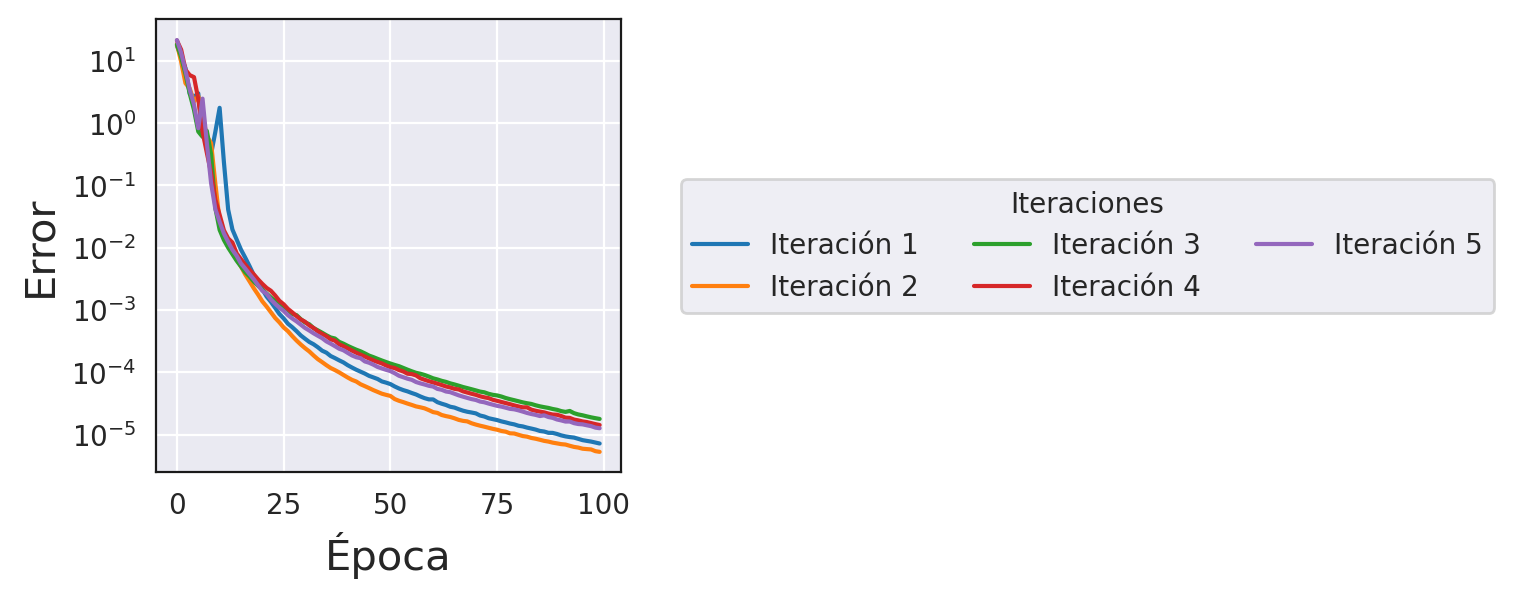
\includegraphics[scale=0.67]{imagenes/image_classification/synthetic_dataset/loss_alexnet_xavier_adam_00005.png}
    \caption{Evolución del error de \textit{training} durante el entrenamiento de un modelo con configuración AlexNet-Xavier-Adam-0.00005 sobre un \textit{dataset} con \textit{hard negatives}.}
    \label{fig:synthetic-loss_alexnet_xavier_adam_00005}
\end{figure}

Se observa como el error decrece suavemente. Elijo esta configuración y se procede a entrenar el modelo final, obteniendo los siguientes resultados:

\begin{table}[H]
    \footnotesize
    \centering
    \caption{Porcentaje de error del modelo final con \textit{hard negatives}.}
\begin{tabular}{@{}ll@{}}
\toprule
Modelo final              & \multicolumn{1}{c}{\begin{tabular}[c]{@{}c@{}}Error sobre la\\ partición de \textit{test}\end{tabular}} \\ \midrule
AlexNet-Xavier-Adam-0.00005 & 0.917\%                                                                                        \\ \bottomrule
\end{tabular}
\end{table}

\begin{figure}[H]
\centering
    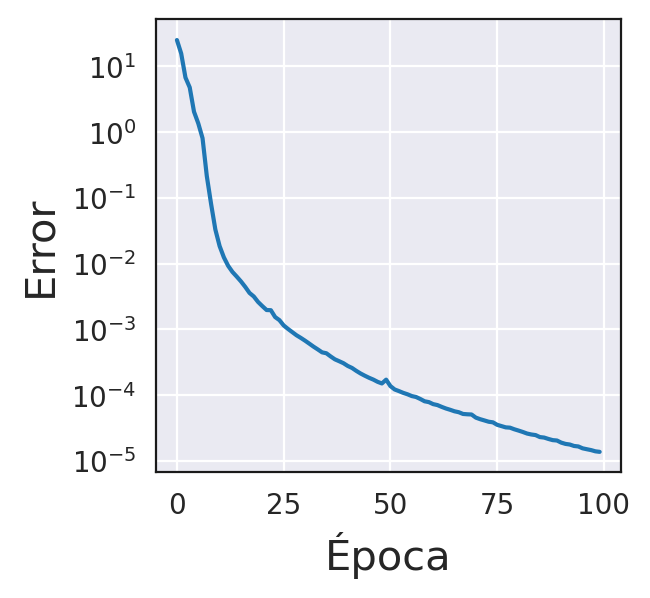
\includegraphics[scale=0.67]{imagenes/image_classification/synthetic_dataset/loss_final_model.png}
    \caption{Evolución del error de \textit{training} durante el entrenamiento del modelo final sobre el \textit{dataset} con \textit{hard negatives}.}
\end{figure}

Da la casualidad de que sobre ambos \textit{datasets}, con y sin \textit{hard negatives}, el modelo escogido utiliza la misma configuración.  Entregaremos a los científicos de la Universidad de Negev ambos modelos.